% Created 2018-06-21 Thu 12:30
\documentclass[8pt]{beamer}
\usepackage[sc,osf]{mathpazo}   % With old-style figures and real smallcaps.
\linespread{1.025}              % Palatino leads a little more leading
% Euler for math and numbers
\usepackage[euler-digits,small]{eulervm}
%\documentclass[10pt]{llncs}
%\usepackage{llncsdoc}
\usepackage{minted}
\usepackage[utf8]{inputenc}
\usepackage[T1]{fontenc}
\usepackage{fixltx2e}
\usepackage{graphicx}
\usepackage{longtable}
\usepackage{float}
\usepackage{wrapfig}
\usepackage{rotating}
\usepackage[normalem]{ulem}
\usepackage{amsmath}
\usepackage{textcomp}
\usepackage{marvosym}
\usepackage{wasysym}
\usepackage{amssymb}
\usepackage{hyperref}
\usepackage{polynom}
\renewcommand{\mod}[1]{\left( \texttt{mod}~#1 \right)}
\newcommand{\N}{\mathbb N}
\newcommand{\Z}{\mathbb Z}
\newcommand{\Q}{\mathbb Q}
\newcommand{\C}{\mathbb C}
\newcommand{\degree}{\texttt{degree}}
\newcommand{\node}{\texttt{node}}
\newcommand{\class}{\texttt{class}}
\newcommand{\egg}{\texttt{egg} }
\tolerance=1000
%\usetheme{Antibes}
\addtobeamertemplate{navigation symbols}{}{%
    \usebeamerfont{footline}%
    \usebeamercolor[fg]{footline}%
    \hspace{1em}%
    \insertframenumber/\inserttotalframenumber
}

\newcommand{\code}[1]{\mintinline{cpp}{#1}}


\author{Siddharth Bhat}
\date{Monday, Jan 18 2021}
\title{\egg: Fast and extensible equality saturation}
\hypersetup{
  pdfkeywords={},
  pdfsubject={},
  pdfcreator={Emacs 24.5.1 (Org mode 8.2.10)}}
\begin{document}

\titlegraphic{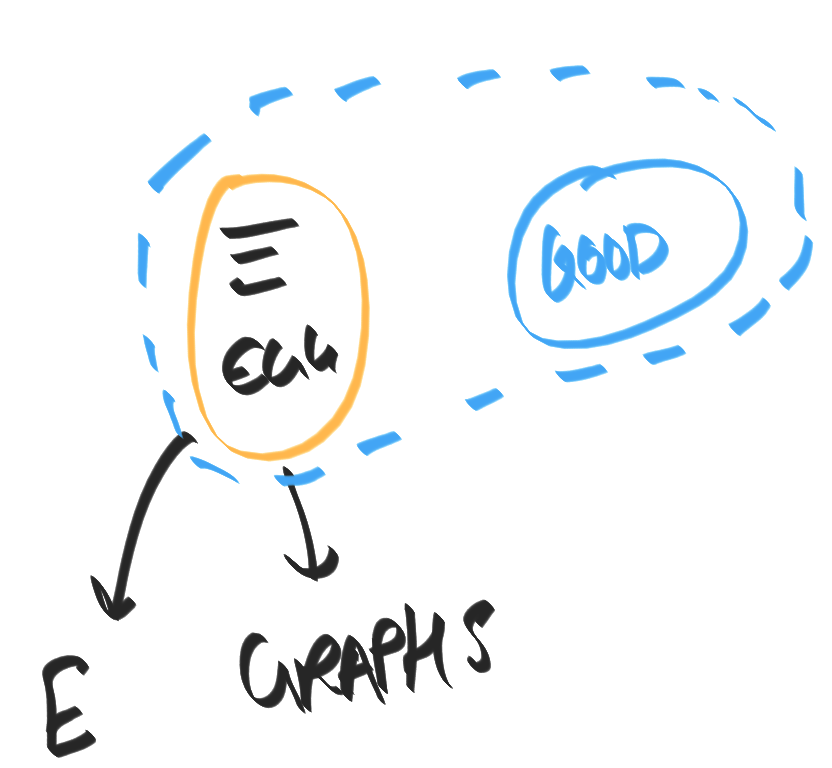
\includegraphics[width=.3\textwidth,height=.3\textheight]{./e-graphs-good.png}}


\maketitle

\begin{frame}[fragile]{How do compilers work?}
\begin{minted}{cpp}
int foo() {
    int x = 1;
    if (x == 1)
        printf("foo")
    else
        printf("bar")
}
\end{minted}

\pause

\begin{minted}{cpp}
int foo() {
    if (1 == 1) // 1. constant propagation
        printf("foo")
    else
        printf("bar")
}
\end{minted}

\pause

\begin{minted}{cpp}
int foo() {
    if (true) // 2. Canonicalization
        printf("foo")
    else
        printf("bar")
}
\end{minted}

\pause

\begin{minted}{cpp}
int main() {
    // 3. control flow simplification
    printf("foo")
}
\end{minted}

\pause
$$
P_0
\xrightarrow{T_1}         P_1
\xrightarrow{T_2}         P_2
\xrightarrow{T_3}         P_3
\xrightarrow{T_4}         P_4
\xrightarrow{\dots}
\dots
$$
\end{frame}

\begin{frame}[fragile]{In what \emph{order}?}
\begin{columns}[T] % align columns
\begin{column}{.48\textwidth}
\begin{minted}[fontsize=\footnotesize]{cpp}
int foo() {
    int x = 1;
    if (x == 1)
        printf("foo")
    else
        printf("bar")
}
\end{minted}
\end{column}

%%%%%%
\begin{column}{.48\textwidth}
\begin{minted}[fontsize=\footnotesize]{cpp}
int bar() {
    int y = 42 == 42;
    if (y)
        printf("foo");
    else
        printf("bar");
}
\end{minted}
\end{column}
\end{columns}
\pause

%%%%%%%%%%%%%%%%%%%%%
%%%%%%%%%%%%%%%%%%%%%

\begin{columns}[T] % align columns
\begin{column}{.48\textwidth}
\begin{minted}[fontsize=\footnotesize]{cpp}
int foo() {
    // 1. constant propagation
    if (1 == 1)
        printf("foo")
    else
        printf("bar")
}
\end{minted}
\end{column}
%%%%%
\begin{column}{.48\textwidth}
\begin{minted}[fontsize=\footnotesize]{cpp}
int bar(int x) {
    // 1. Constant propagation
    int y = x == x;
    if (y)  // NOT a constant!
        printf("foo");
    else
        printf("bar");
}
\end{minted}
\end{column}
\end{columns}
\pause


\begin{columns}
\begin{column}{.48\textwidth}
\begin{minted}[fontsize=\footnotesize]{cpp}
int foo() {
    // 2. Canonicalization
    if (true)
        printf("foo")
    else
        printf("bar")
}
\end{minted}
\end{column}
%%%%%
\begin{column}{.48\textwidth}
\begin{minted}[fontsize=\footnotesize]{cpp}
int bar(int x) {
    // 2. Canonicalization
    int y = true;
    if (y)  
        printf("foo");
    else
        printf("bar");
}
\end{minted}
\end{column}
\end{columns}

%%%%%%%%%%%
%%%%%%%%%%%


\pause
\begin{columns}
\begin{column}{.48\textwidth}
\begin{minted}[fontsize=\footnotesize]{cpp}
int main() {
    // 3. control flow simplification
    printf("foo")
}
\end{minted}
\end{column}
%%%%%
\begin{column}{.48\textwidth}
\begin{minted}[fontsize=\footnotesize]{cpp}
int bar(int x) {
    int y = true;
    // 3. Control flow simplification
    if (y) // Cannot simplify control flow. 
        printf("foo");
    else
        printf("bar");
}
\end{minted}
\end{column}
\end{columns}
\end{frame}


\begin{frame}[fragile]{In what \emph{Order}? All of them}
\begin{columns}[T] % align columns
\begin{column}{.48\textwidth}
\begin{minted}[fontsize=\footnotesize]{cpp}
int bar() {
    int y = 42 == 42;
    if (y)
        printf("foo");
    else
        printf("bar");
}
\end{minted}
\end{column}
\pause
\begin{column}{.48\textwidth}
\begin{minted}[fontsize=\footnotesize]{cpp}
int bar(int x) {
    // 1. Constant propagation
    int y = x == x;
    if (y) // NOT a constant!
        printf("foo");
    else
        printf("bar");
}
\end{minted}
\end{column}
\end{columns}
\pause

\begin{columns}[T] % align columns
\begin{column}{.48\textwidth}
\begin{minted}[fontsize=\footnotesize]{cpp}
int bar(int x) {
    // 2. Canonicalization
    int y = true;
    if (y)
        printf("foo");
    else
        printf("bar");
}
\end{minted}
\end{column}
\pause
\begin{column}{.48\textwidth}
\begin{minted}[fontsize=\footnotesize]{cpp}
int bar(int x) {
    int y = true;
    // 3. Control flow simplification
    if (y) // Cannot simplify control flow.
        printf("foo");
    else
        printf("bar");
}
\end{minted}
\end{column}
\end{columns}
\pause
\begin{columns}[T] % align columns
\begin{column}{.48\textwidth}
\begin{minted}[fontsize=\footnotesize]{cpp}
int bar(int x) {
    // 4. Constant propagation
    int y = true;
    if (true)  // IS a constant now!
        printf("foo");
    else
        printf("bar");
}
\end{minted}
\end{column}

\pause
\begin{column}{.48\textwidth}
\begin{minted}[fontsize=\footnotesize]{cpp}
int bar(int x) {
    int y = true;
    // 5. Control flow simplification
    printf("foo");
}
\end{minted}
\end{column}
\end{columns}
\end{frame}

\begin{frame}[fragile]{Solutions to the phase ordering problem}

\pause
\begin{minted}[fontsize=\tiny]{text}
bollu@cantordust:~/ > clang  -O3 -mllvm -debug-pass=Arguments ~/temp/foo.c
\end{minted}
\pause
\begin{minted}[fontsize=\tiny]{text}
bollu@cantordust:~/ > clang  -O3 -mllvm -debug-pass=Arguments ~/temp/foo.c
Pass Arguments:  -tti -targetlibinfo -tbaa -scoped-noalias-aa
-instcombine -simplifycfg -basiccg -globals-aa -prune-eh -inline -openmpopt
-function-attrs -argpromotion -domtree -sroa -basic-aa -aa -memoryssa
-early-cse-memssa -aa -lazy-value-info -jump-threading -correlated-propagation
-simplifycfg -domtree -aggressive-instcombine -basic-aa -aa -loops
-lazy-branch-prob -lazy-block-freq -opt-remark-emitter -instcombine
-libcalls-shrinkwrap -loops -postdomtree -branch-prob -block-freq
-lazy-branch-prob -lazy-block-freq -opt-remark-emitter -pgo-memop-opt -basic-aa
-aa -loops -lazy-branch-prob -lazy-block-freq -opt-remark-emitter -tailcallelim
-simplifycfg -reassociate -domtree -loops -loop-simplify -lcssa-verification
-lcssa -basic-aa -aa -scalar-evolution -loop-rotate -memoryssa
-lazy-branch-prob -lazy-block-freq -licm -loop-unswitch -simplifycfg -domtree
-basic-aa -aa -loops -lazy-branch-prob -lazy-block-freq -opt-remark-emitter
-instcombine -loop-simplify -lcssa-verification -lcssa -scalar-evolution
-loop-idiom -indvars -loop-deletion -loop-unroll -sroa -aa -mldst-motion
-phi-values -aa -memdep -lazy-branch-prob -lazy-block-freq -opt-remark-emitter
-gvn -phi-values -basic-aa -aa -memdep -memcpyopt -sccp -demanded-bits -bdce
-aa -lazy-branch-prob -lazy-block-freq -opt-remark-emitter -instcombine
-lazy-value-info -jump-threading -correlated-propagation -postdomtree -adce
-basic-aa -aa -memoryssa -dse -loops -loop-simplify -lcssa-verification -lcssa
-aa -scalar-evolution -lazy-branch-prob -lazy-block-freq -licm -simplifycfg
-domtree -basic-aa -aa -loops -lazy-branch-prob -lazy-block-freq
-opt-remark-emitter -instcombine -barrier -elim-avail-extern -basiccg
-rpo-function-attrs -globalopt -globaldce -basiccg -globals-aa -domtree
-float2int -lower-constant-intrinsics -domtree -loops -loop-simplify
-lcssa-verification -lcssa -basic-aa -aa -scalar-evolution -loop-rotate
-loop-accesses -lazy-branch-prob -lazy-block-freq -opt-remark-emitter
-loop-distribute -postdomtree -branch-prob -block-freq -scalar-evolution
-basic-aa -aa -loop-accesses -demanded-bits -lazy-branch-prob -lazy-block-freq
-opt-remark-emitter -inject-tli-mappings -loop-vectorize -loop-simplify
-scalar-evolution -aa -loop-accesses -lazy-branch-prob -lazy-block-freq
-loop-load-elim -basic-aa -aa -lazy-branch-prob -lazy-block-freq
-opt-remark-emitter -instcombine -simplifycfg -domtree -loops -scalar-evolution
-basic-aa -aa -demanded-bits -lazy-branch-prob -lazy-block-freq
-opt-remark-emitter -inject-tli-mappings -slp-vectorizer -vector-combine
-opt-remark-emitter -instcombine -loop-simplify -lcssa-verification -lcssa
...
\end{minted}
\end{frame}

\begin{frame}[fragile]{Solutions to the phase ordering problem}
\begin{minted}[fontsize=\tiny]{text}
bollu@cantordust:~/ > clang  -O3 -mllvm -debug-pass=Arguments ~/temp/foo.c
\end{minted}
\begin{minted}[fontsize=\tiny]{text}
bollu@cantordust:~/ > clang  -O3 -mllvm -debug-pass=Arguments ~/temp/foo.c
Pass Arguments:                                               
-instcombine                                                                
                                                                     
                                                                              
                                                                  
                                                       -instcombine
                                                                 
                                                                               
                                                                               
                                                                            
                                                              
                                                                             
                                                                           
-instcombine                                                             
                                                                        
                                                                              
                                                                            
                                                           -instcombine
                                                                           
                                                                              
                                                                           
                                                                
                    -instcombine                                      
                                                                       
                                                                    
                                                                       
                                                                     
                                                                        
                                                                              
                                                                       
                                                                       
                                                                
                    -instcombine                                               
                                                               
                                                                        
                    -instcombine                                          
...
\end{minted}
\end{frame}


\begin{frame}[fragile]{Solutions to the phase ordering problem}
\begin{minted}[fontsize=\tiny]{text}
bollu@cantordust:~/ > clang  -O3 -mllvm -debug-pass=Arguments ~/temp/foo.c
\end{minted}
\begin{minted}[fontsize=\tiny]{text}
bollu@cantordust:~/ > clang  -O3 -mllvm -debug-pass=Arguments ~/temp/foo.c
Pass Arguments:  -tti -targetlibinfo -tbaa -scoped-noalias-aa
-instcombine -simplifycfg -basiccg -globals-aa -prune-eh -inline -openmpopt
-function-attrs -argpromotion -domtree -sroa -basic-aa -aa -memoryssa
-early-cse-memssa -aa -lazy-value-info -jump-threading -correlated-propagation
-simplifycfg -domtree -aggressive-instcombine -basic-aa -aa -loops
-lazy-branch-prob -lazy-block-freq -opt-remark-emitter -instcombine
-libcalls-shrinkwrap -loops -postdomtree -branch-prob -block-freq
-lazy-branch-prob -lazy-block-freq -opt-remark-emitter -pgo-memop-opt -basic-aa
-aa -loops -lazy-branch-prob -lazy-block-freq -opt-remark-emitter -tailcallelim
-simplifycfg -reassociate -domtree -loops -loop-simplify -lcssa-verification
-lcssa -basic-aa -aa -scalar-evolution -loop-rotate -memoryssa
-lazy-branch-prob -lazy-block-freq -licm -loop-unswitch -simplifycfg -domtree
-basic-aa -aa -loops -lazy-branch-prob -lazy-block-freq -opt-remark-emitter
-instcombine -loop-simplify -lcssa-verification -lcssa -scalar-evolution
-loop-idiom -indvars -loop-deletion -loop-unroll -sroa -aa -mldst-motion
-phi-values -aa -memdep -lazy-branch-prob -lazy-block-freq -opt-remark-emitter
-gvn -phi-values -basic-aa -aa -memdep -memcpyopt -sccp -demanded-bits -bdce
-aa -lazy-branch-prob -lazy-block-freq -opt-remark-emitter -instcombine
-lazy-value-info -jump-threading -correlated-propagation -postdomtree -adce
-basic-aa -aa -memoryssa -dse -loops -loop-simplify -lcssa-verification -lcssa
-aa -scalar-evolution -lazy-branch-prob -lazy-block-freq -licm -simplifycfg
-domtree -basic-aa -aa -loops -lazy-branch-prob -lazy-block-freq
-opt-remark-emitter -instcombine -barrier -elim-avail-extern -basiccg
-rpo-function-attrs -globalopt -globaldce -basiccg -globals-aa -domtree
-float2int -lower-constant-intrinsics -domtree -loops -loop-simplify
-lcssa-verification -lcssa -basic-aa -aa -scalar-evolution -loop-rotate
-loop-accesses -lazy-branch-prob -lazy-block-freq -opt-remark-emitter
-loop-distribute -postdomtree -branch-prob -block-freq -scalar-evolution
-basic-aa -aa -loop-accesses -demanded-bits -lazy-branch-prob -lazy-block-freq
-opt-remark-emitter -inject-tli-mappings -loop-vectorize -loop-simplify
-scalar-evolution -aa -loop-accesses -lazy-branch-prob -lazy-block-freq
-loop-load-elim -basic-aa -aa -lazy-branch-prob -lazy-block-freq
-opt-remark-emitter -instcombine -simplifycfg -domtree -loops -scalar-evolution
-basic-aa -aa -demanded-bits -lazy-branch-prob -lazy-block-freq
-opt-remark-emitter -inject-tli-mappings -slp-vectorizer -vector-combine
-opt-remark-emitter -instcombine -loop-simplify -lcssa-verification -lcssa
...
\end{minted}
\end{frame}



\begin{frame}[fragile]{Solutions to the phase ordering problem}
\begin{minted}[fontsize=\tiny]{text}
bollu@cantordust:~/ > clang  -O3 -mllvm -debug-pass=Arguments ~/temp/foo.c
\end{minted}
\begin{minted}[fontsize=\tiny]{text}
bollu@cantordust:~/ > clang  -O3 -mllvm -debug-pass=Arguments ~/temp/foo.c
Pass Arguments:                                               
-instcombine -simplifycfg                                                   
                                                                      
                                                                               
-simplifycfg                                                       
                                                       -instcombine
                                                                 
                                                                               
                                                                               
-simplifycfg                                                                 
                                                              
                                                        -simplifycfg          
                                                                           
-instcombine                                                             
                                                                        
                                                                              
                                                                            
                                                           -instcombine
                                                                           
                                                                              
                                                               -simplifycfg
                                                                
                    -instcombine                                      
                                                                       
                                                                    
                                                                       
                                                                     
                                                                        
                                                                              
                                                                       
                                                                       
                                                                
                    -instcombine -simplifycfg                                   
                                                               
                                                                        
                    -instcombine                                           
...
\end{minted}
\end{frame}

\begin{frame}[fragile]{Solutions? to the phase ordering problem}
\begin{itemize}
\item \code{(a*2)/2} \pause
\item \code{(a*2)/2} \pause $\xrightarrow{A}$ \code{(a << 1)/2 } \pause
\item \code{(a*2)/2} \pause $\xrightarrow{B}$ \code{a*(2/2)} \pause $\rightarrow$ \code{a*1} \pause $\rightarrow$ \code{a} \pause
\item \code{(a*2)/2} \pause $\xrightarrow{A}$ \code{(a << 1)/2} \pause $\rightarrow$ \texttt{blocked!} \pause
\item Rerunning \texttt{(pass A; pass B)} multiple times won't help. transformations don't commute!
\item \code{[(a*2)/2} \pause $=_A$  \code{(a*2)/2; (a<<1)/2]} \pause $=_B$ \code{[(a*2)/2; (a<<1)/2; a*(2/2)]} \pause $=$ \code{[(a*2)/2; (a<<1)/2; a*(2/2); a*1]} \pause $=$ \code{[a*(2/2); (a<<1)/2; a*(2/2); a*1; a]} 
\end{itemize}
\end{frame}

\begin{frame}[fragile]{Solutions to the phase ordering problem: Equality saturation}
\begin{itemize}
\item Is \texttt{(pass A; pass B)} is not the same as \texttt{pass B; pass A}.
\item Solution: run all passes "in parallel", at the same time. \pause
\item \emph{saturate} the original program with new programs
      \emph{equivalent} to the original program.
\end{itemize}

\pause
\begin{figure}

\includegraphics[width=0.3\textwidth]{./transform-old.png}
\caption{classical}
\end{figure}
\pause

\begin{columns}
\begin{column}{.48\textwidth}
\begin{figure}
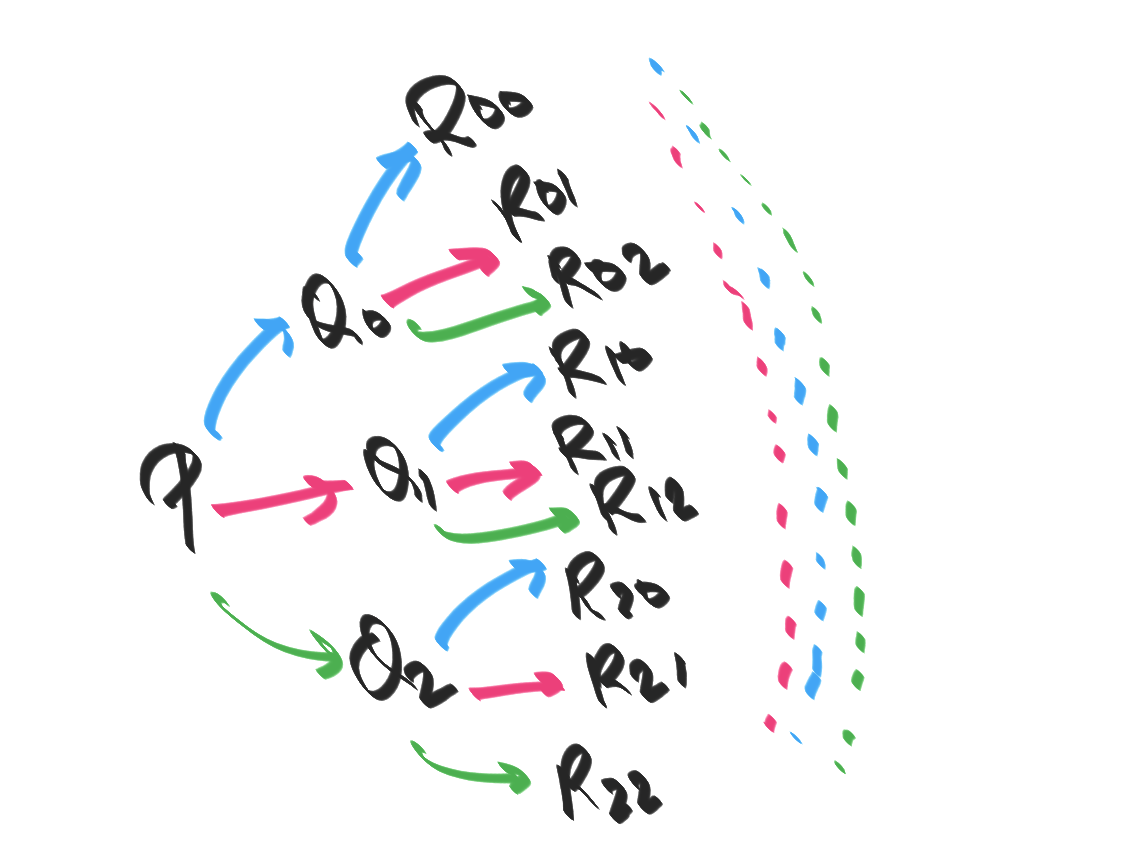
\includegraphics[width=0.5\textwidth]{./transform-new.png}
\caption{all possible transforms}
\end{figure}
\end{column}
\pause
\begin{column}{.48\textwidth}
\begin{figure}
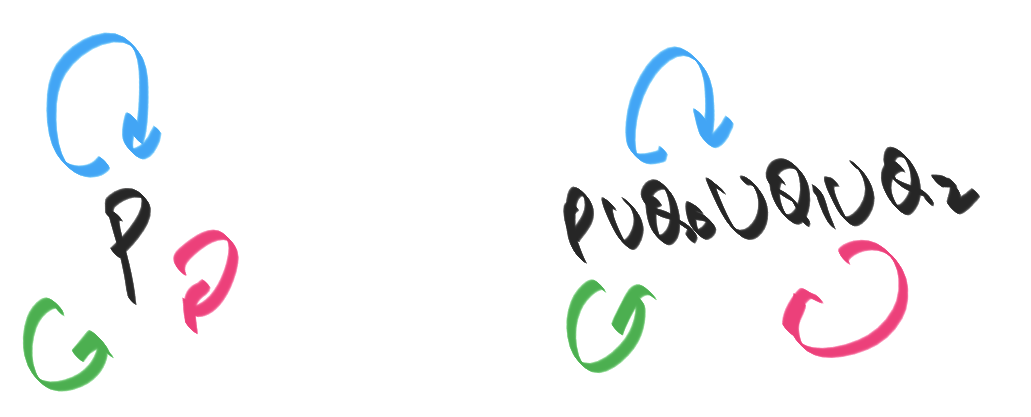
\includegraphics[width=0.7\textwidth]{./transform-eqsat.png}
\caption{equality saturation}
\end{figure}
\end{column}
\end{columns}

\end{frame}


\begin{frame}[fragile]{\egg: Fast and extensible equality saturation}
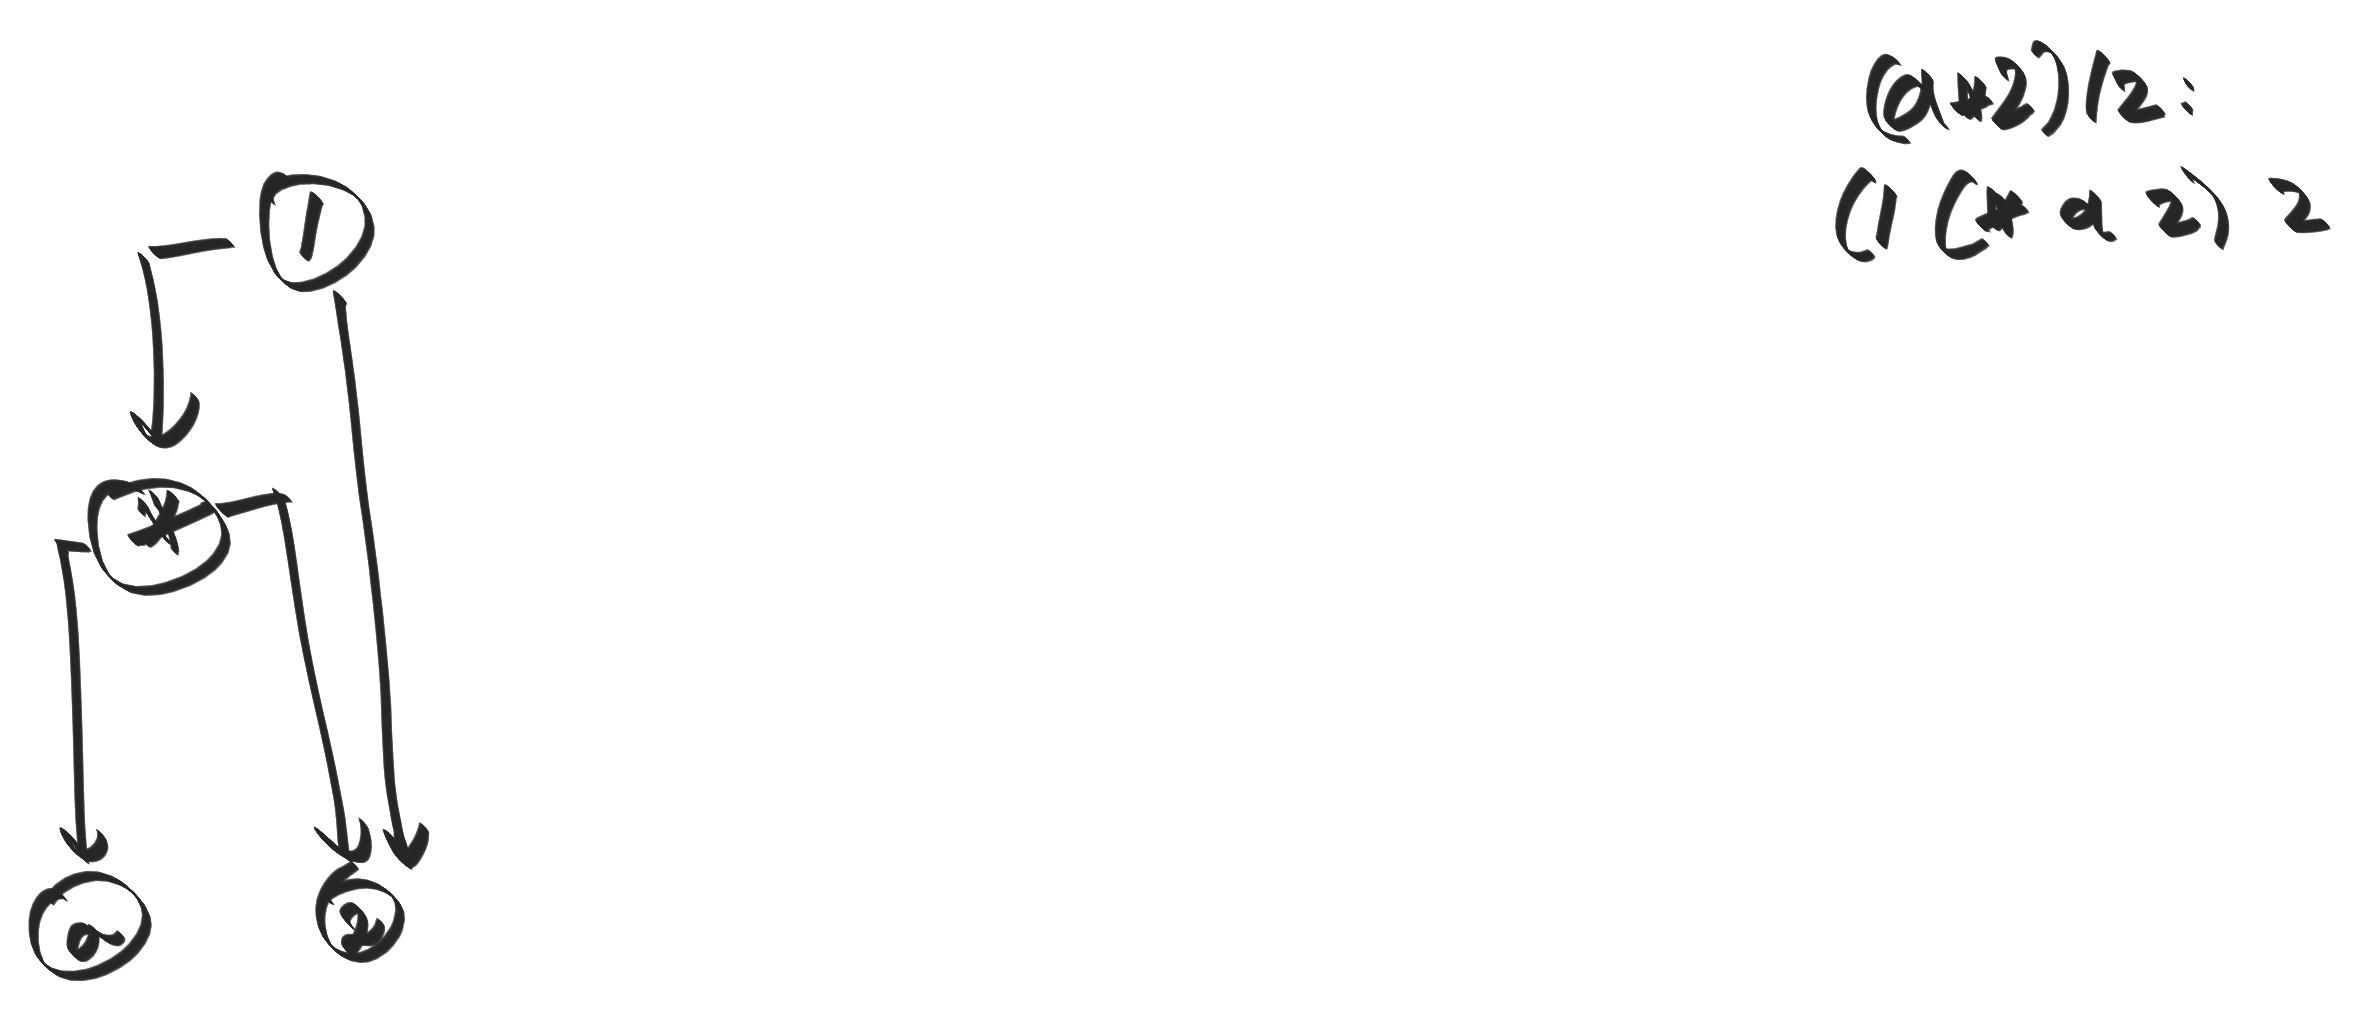
\includegraphics[width=\textwidth]{./eg-1-1.png}
\end{frame}

\begin{frame}[fragile]{\egg: Fast and extensible equality saturation (2)}
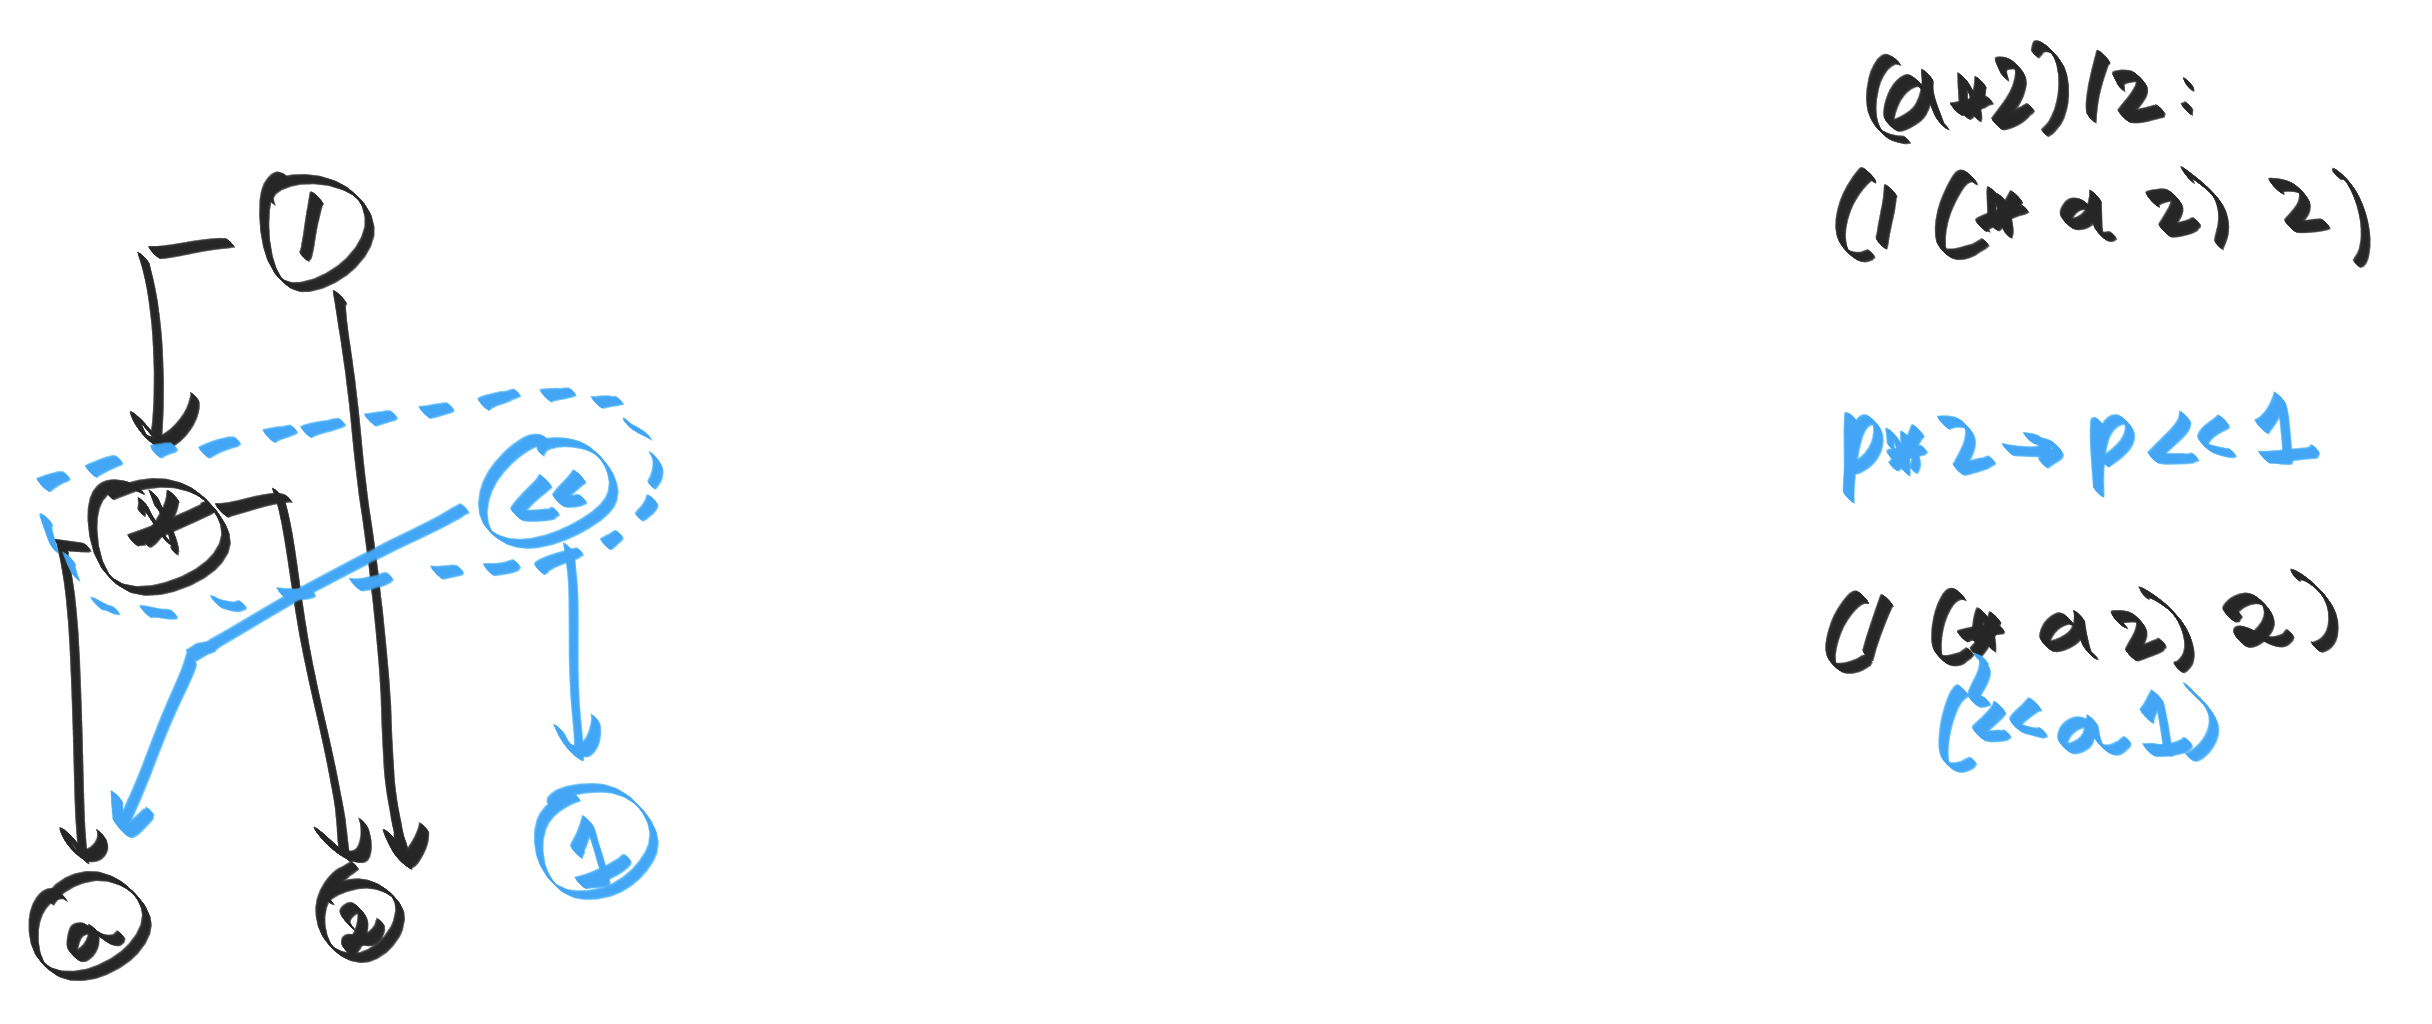
\includegraphics[width=\textwidth]{./eg-1-2.png}
\end{frame}         


\begin{frame}[fragile]{\egg: Fast and extensible equality saturation (3)}
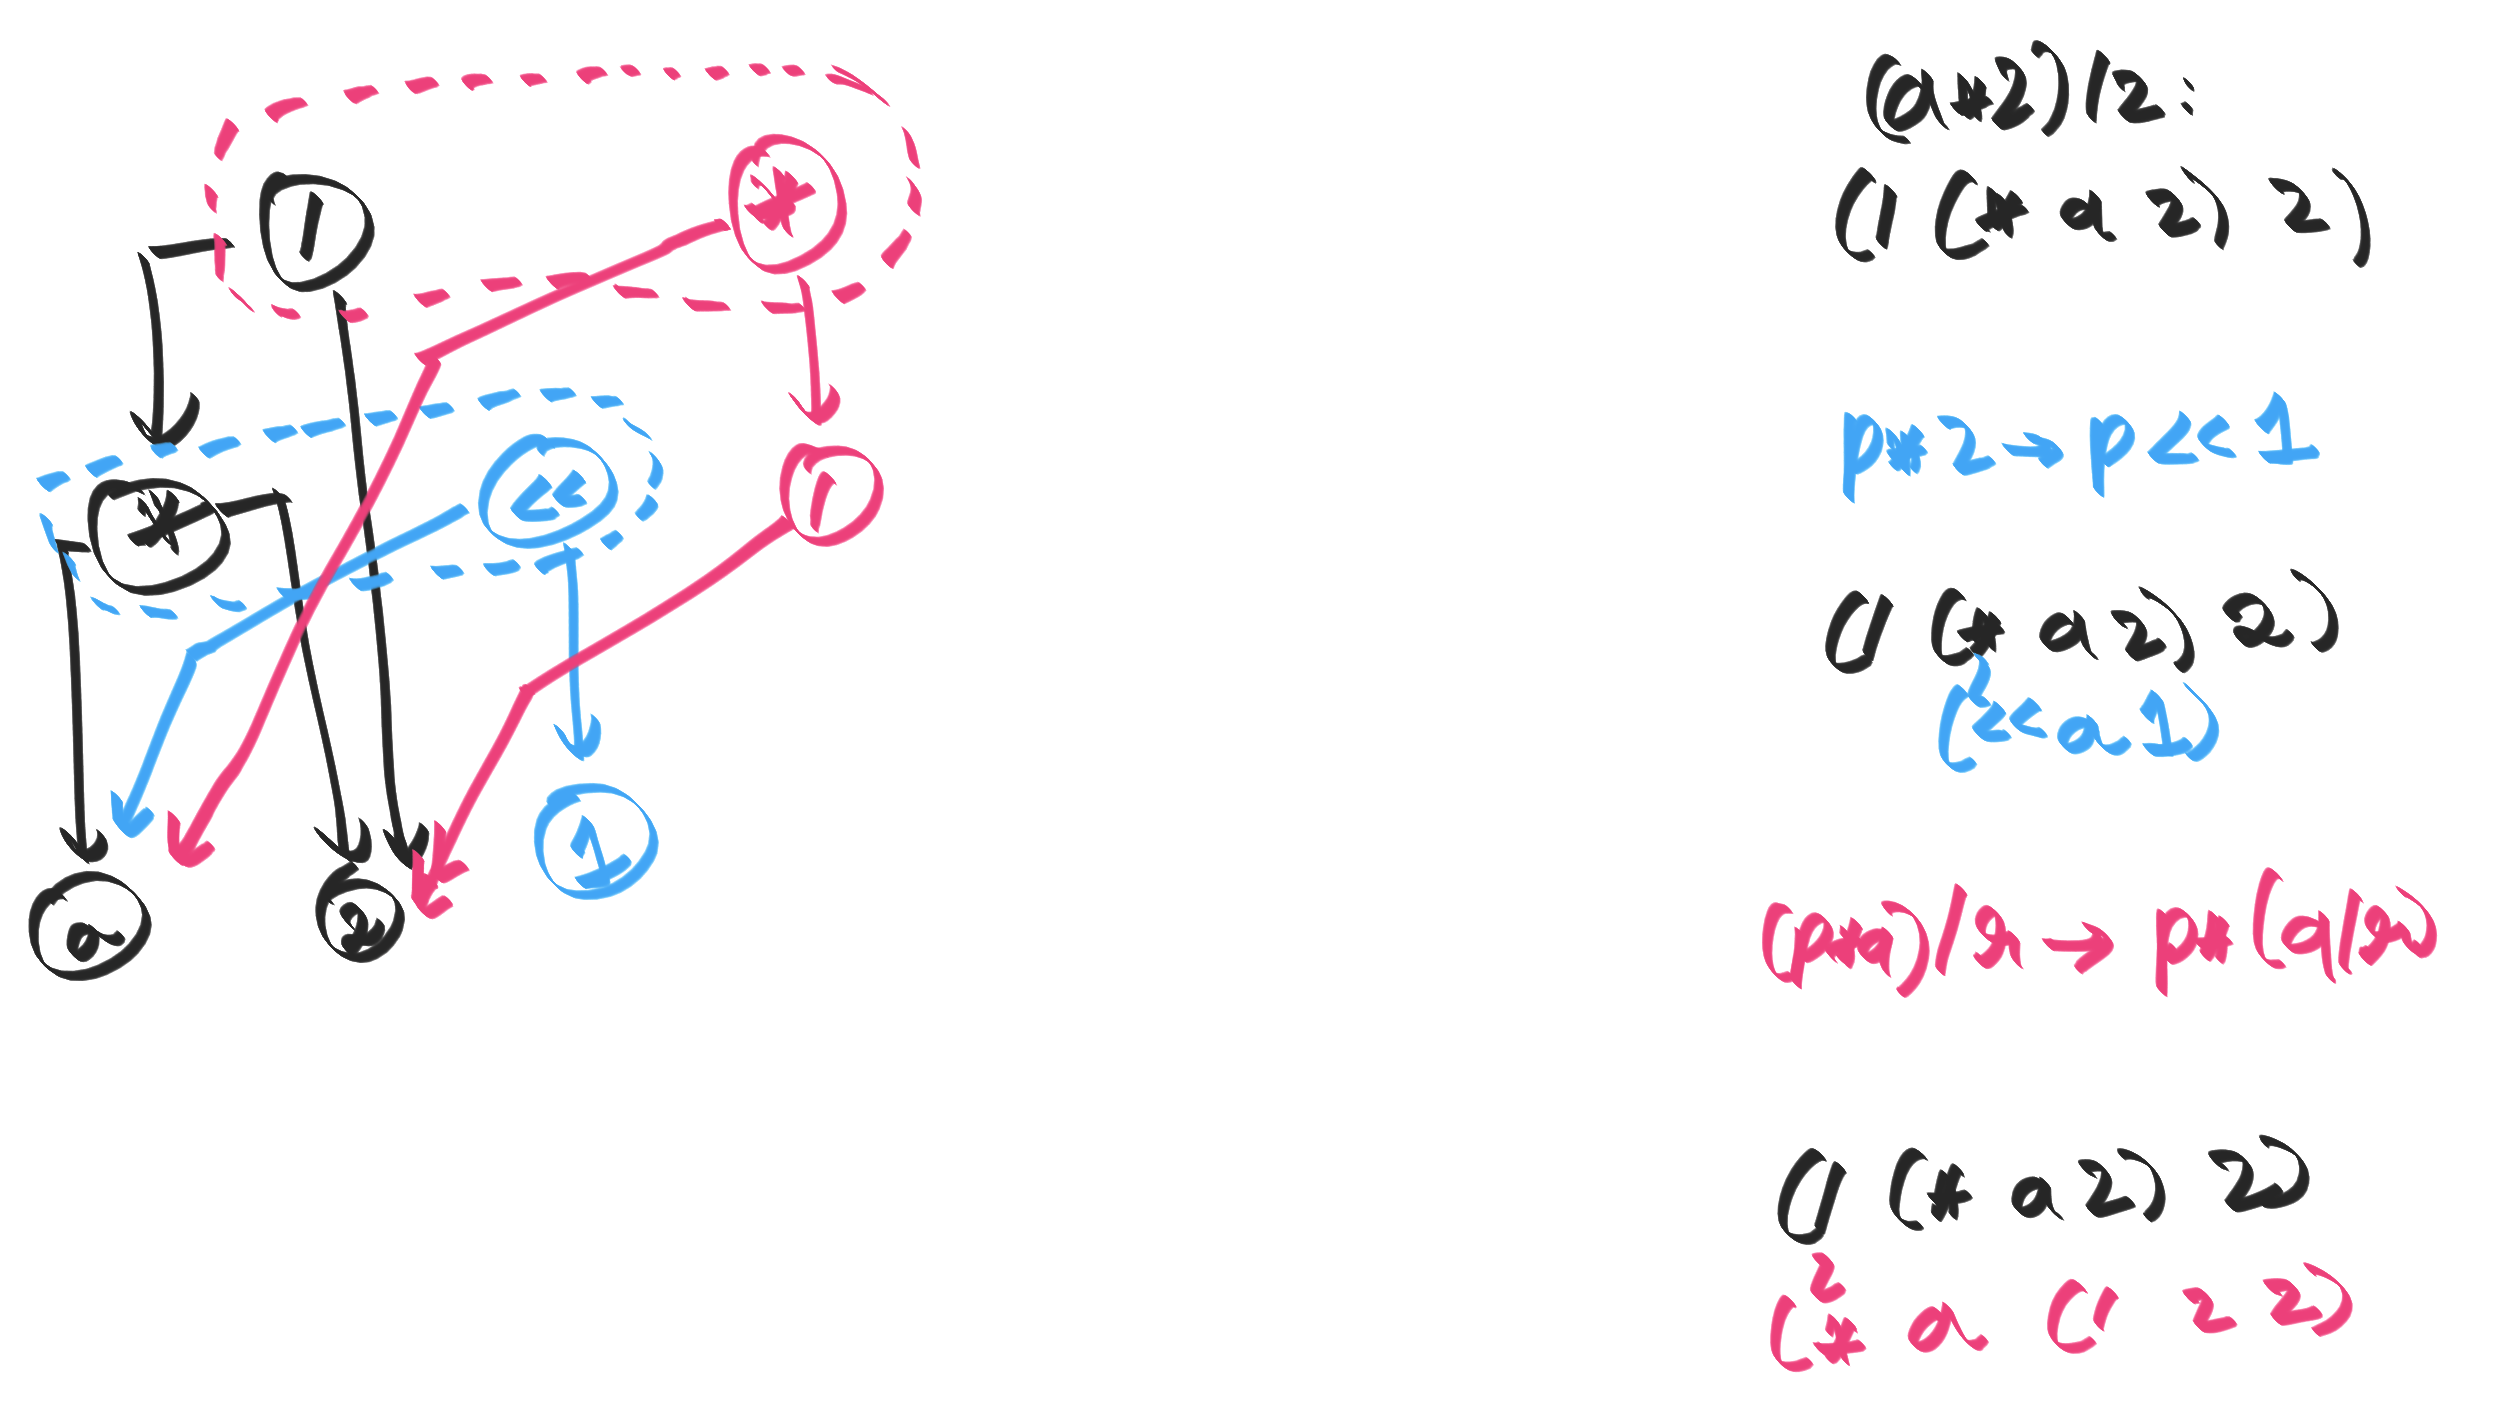
\includegraphics[width=\textwidth]{./eg-1-3.png}
\end{frame}

\begin{frame}[fragile]{\egg: Fast and extensible equality saturation (4)}
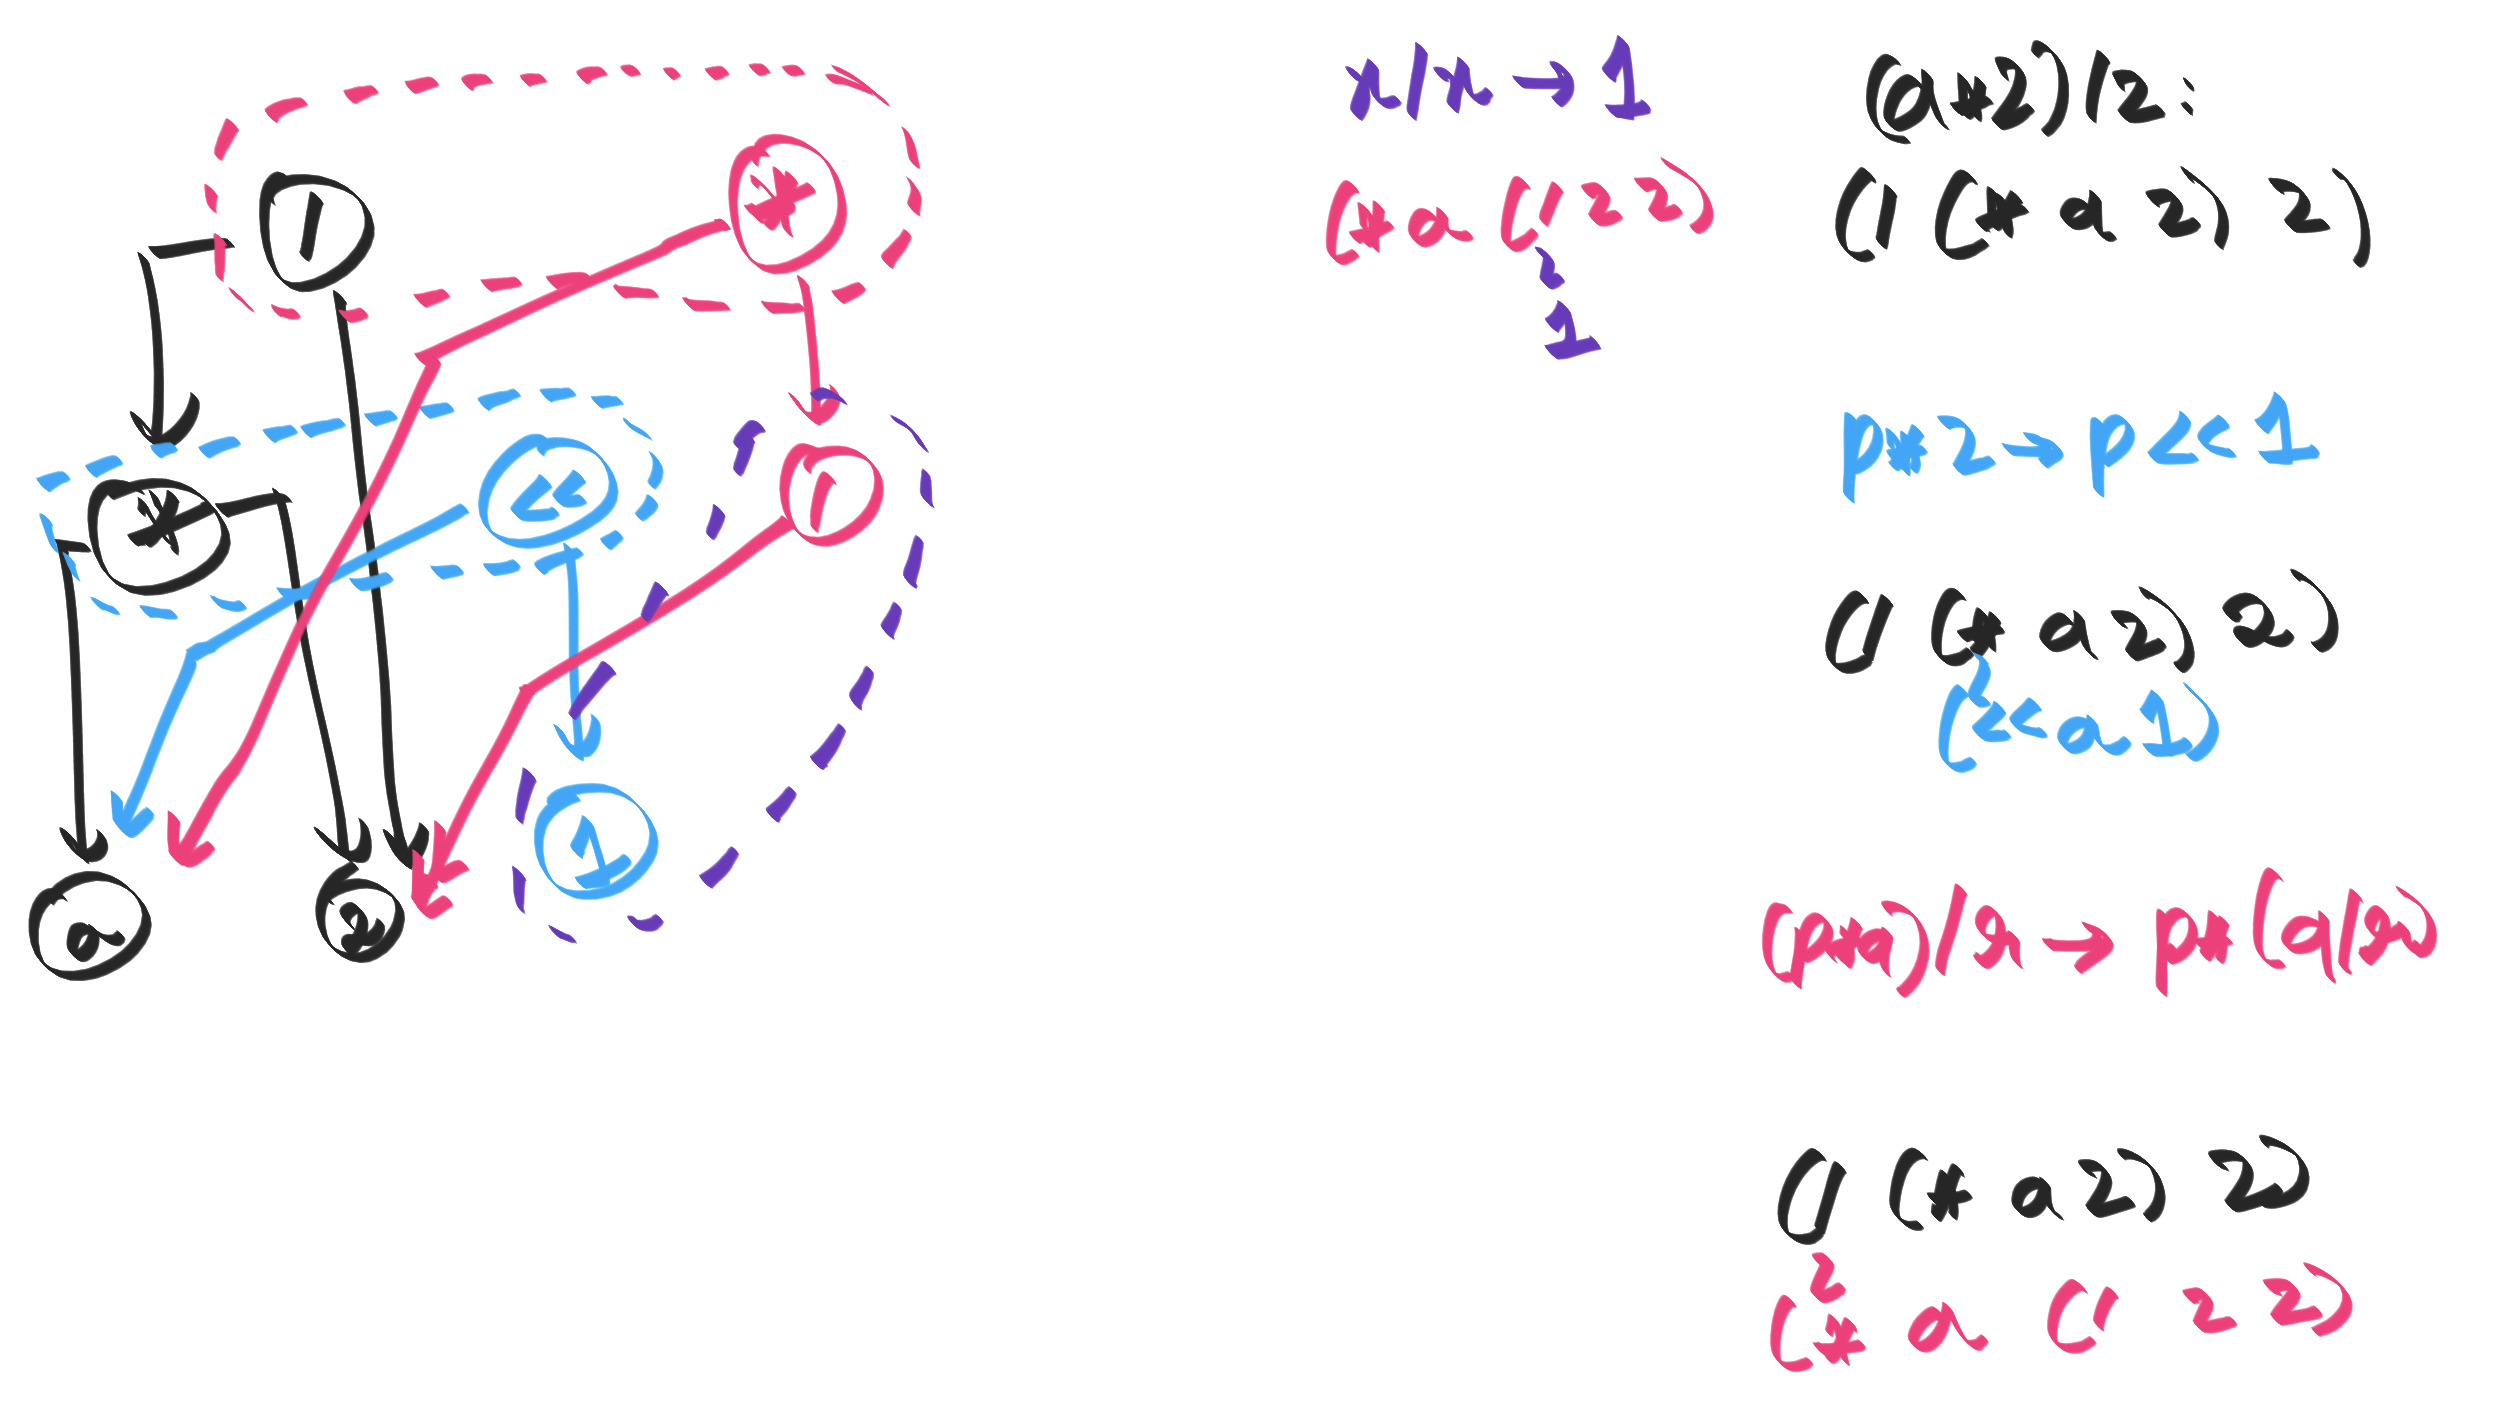
\includegraphics[width=\textwidth]{./eg-1-4.png}
\end{frame}


\begin{frame}[fragile]{\egg: Fast and extensible equality saturation (5)}
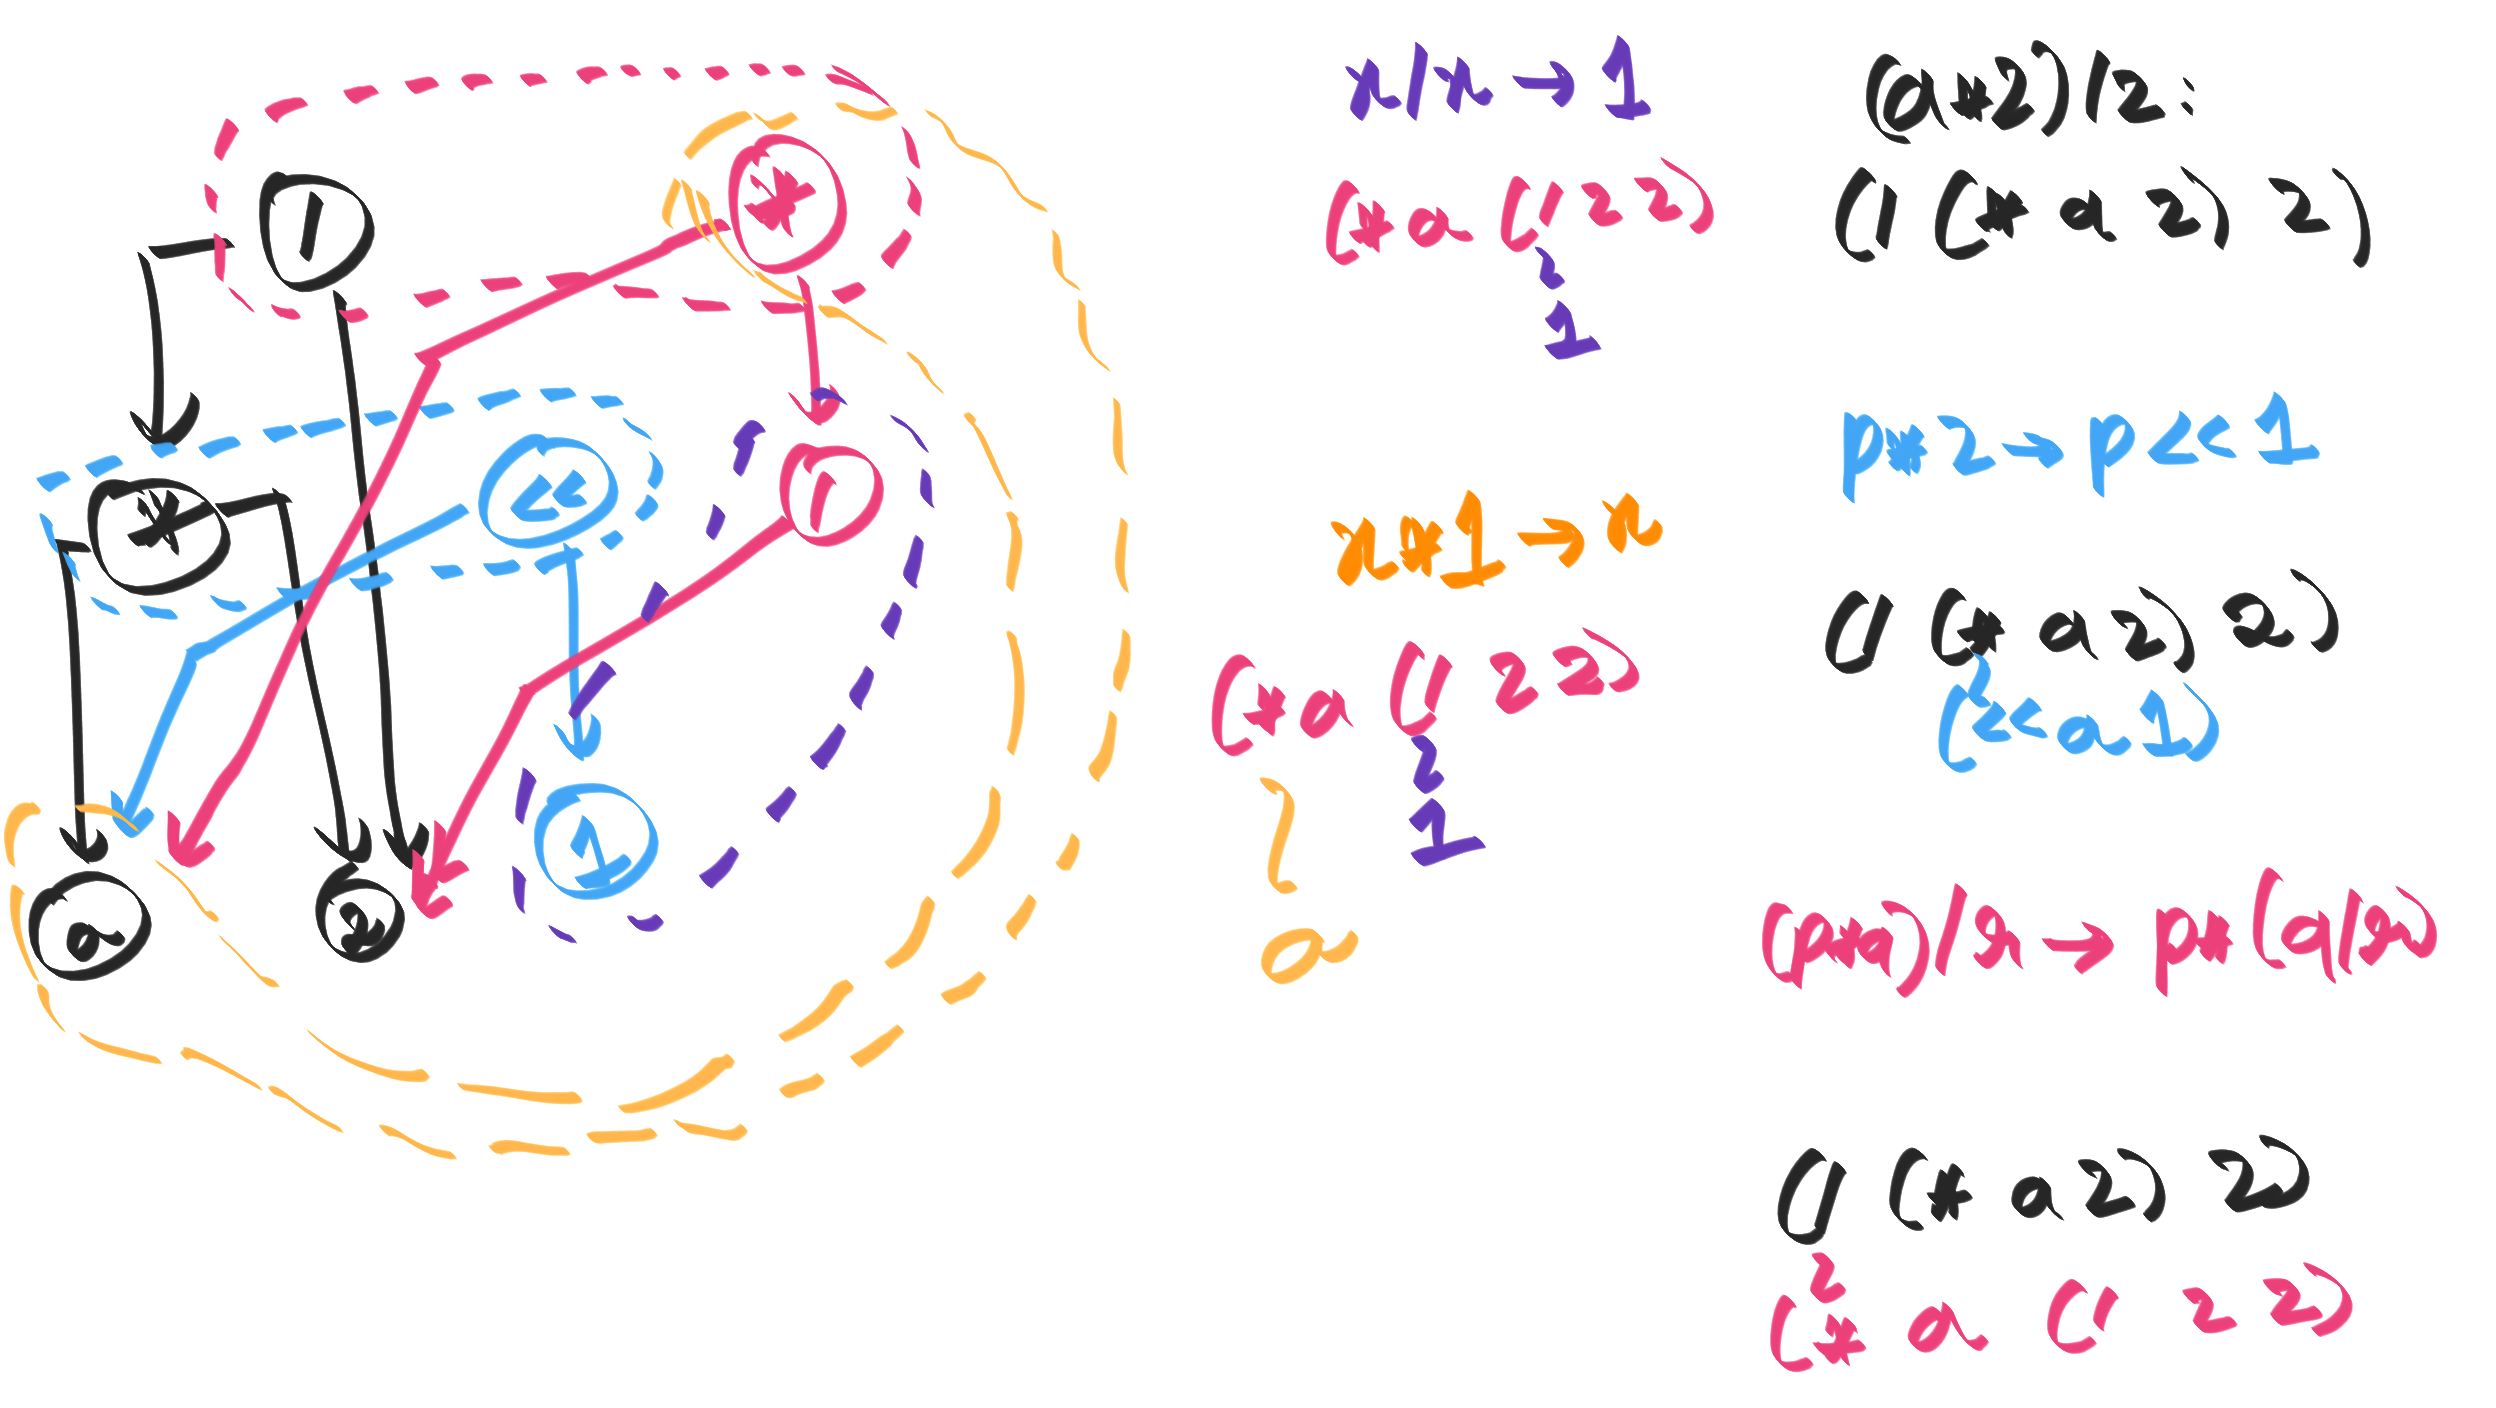
\includegraphics[width=\textwidth]{./eg-1-5.png}
\end{frame}


\begin{frame}[fragile]{\egg: Fast and extensible equality saturation (6)}
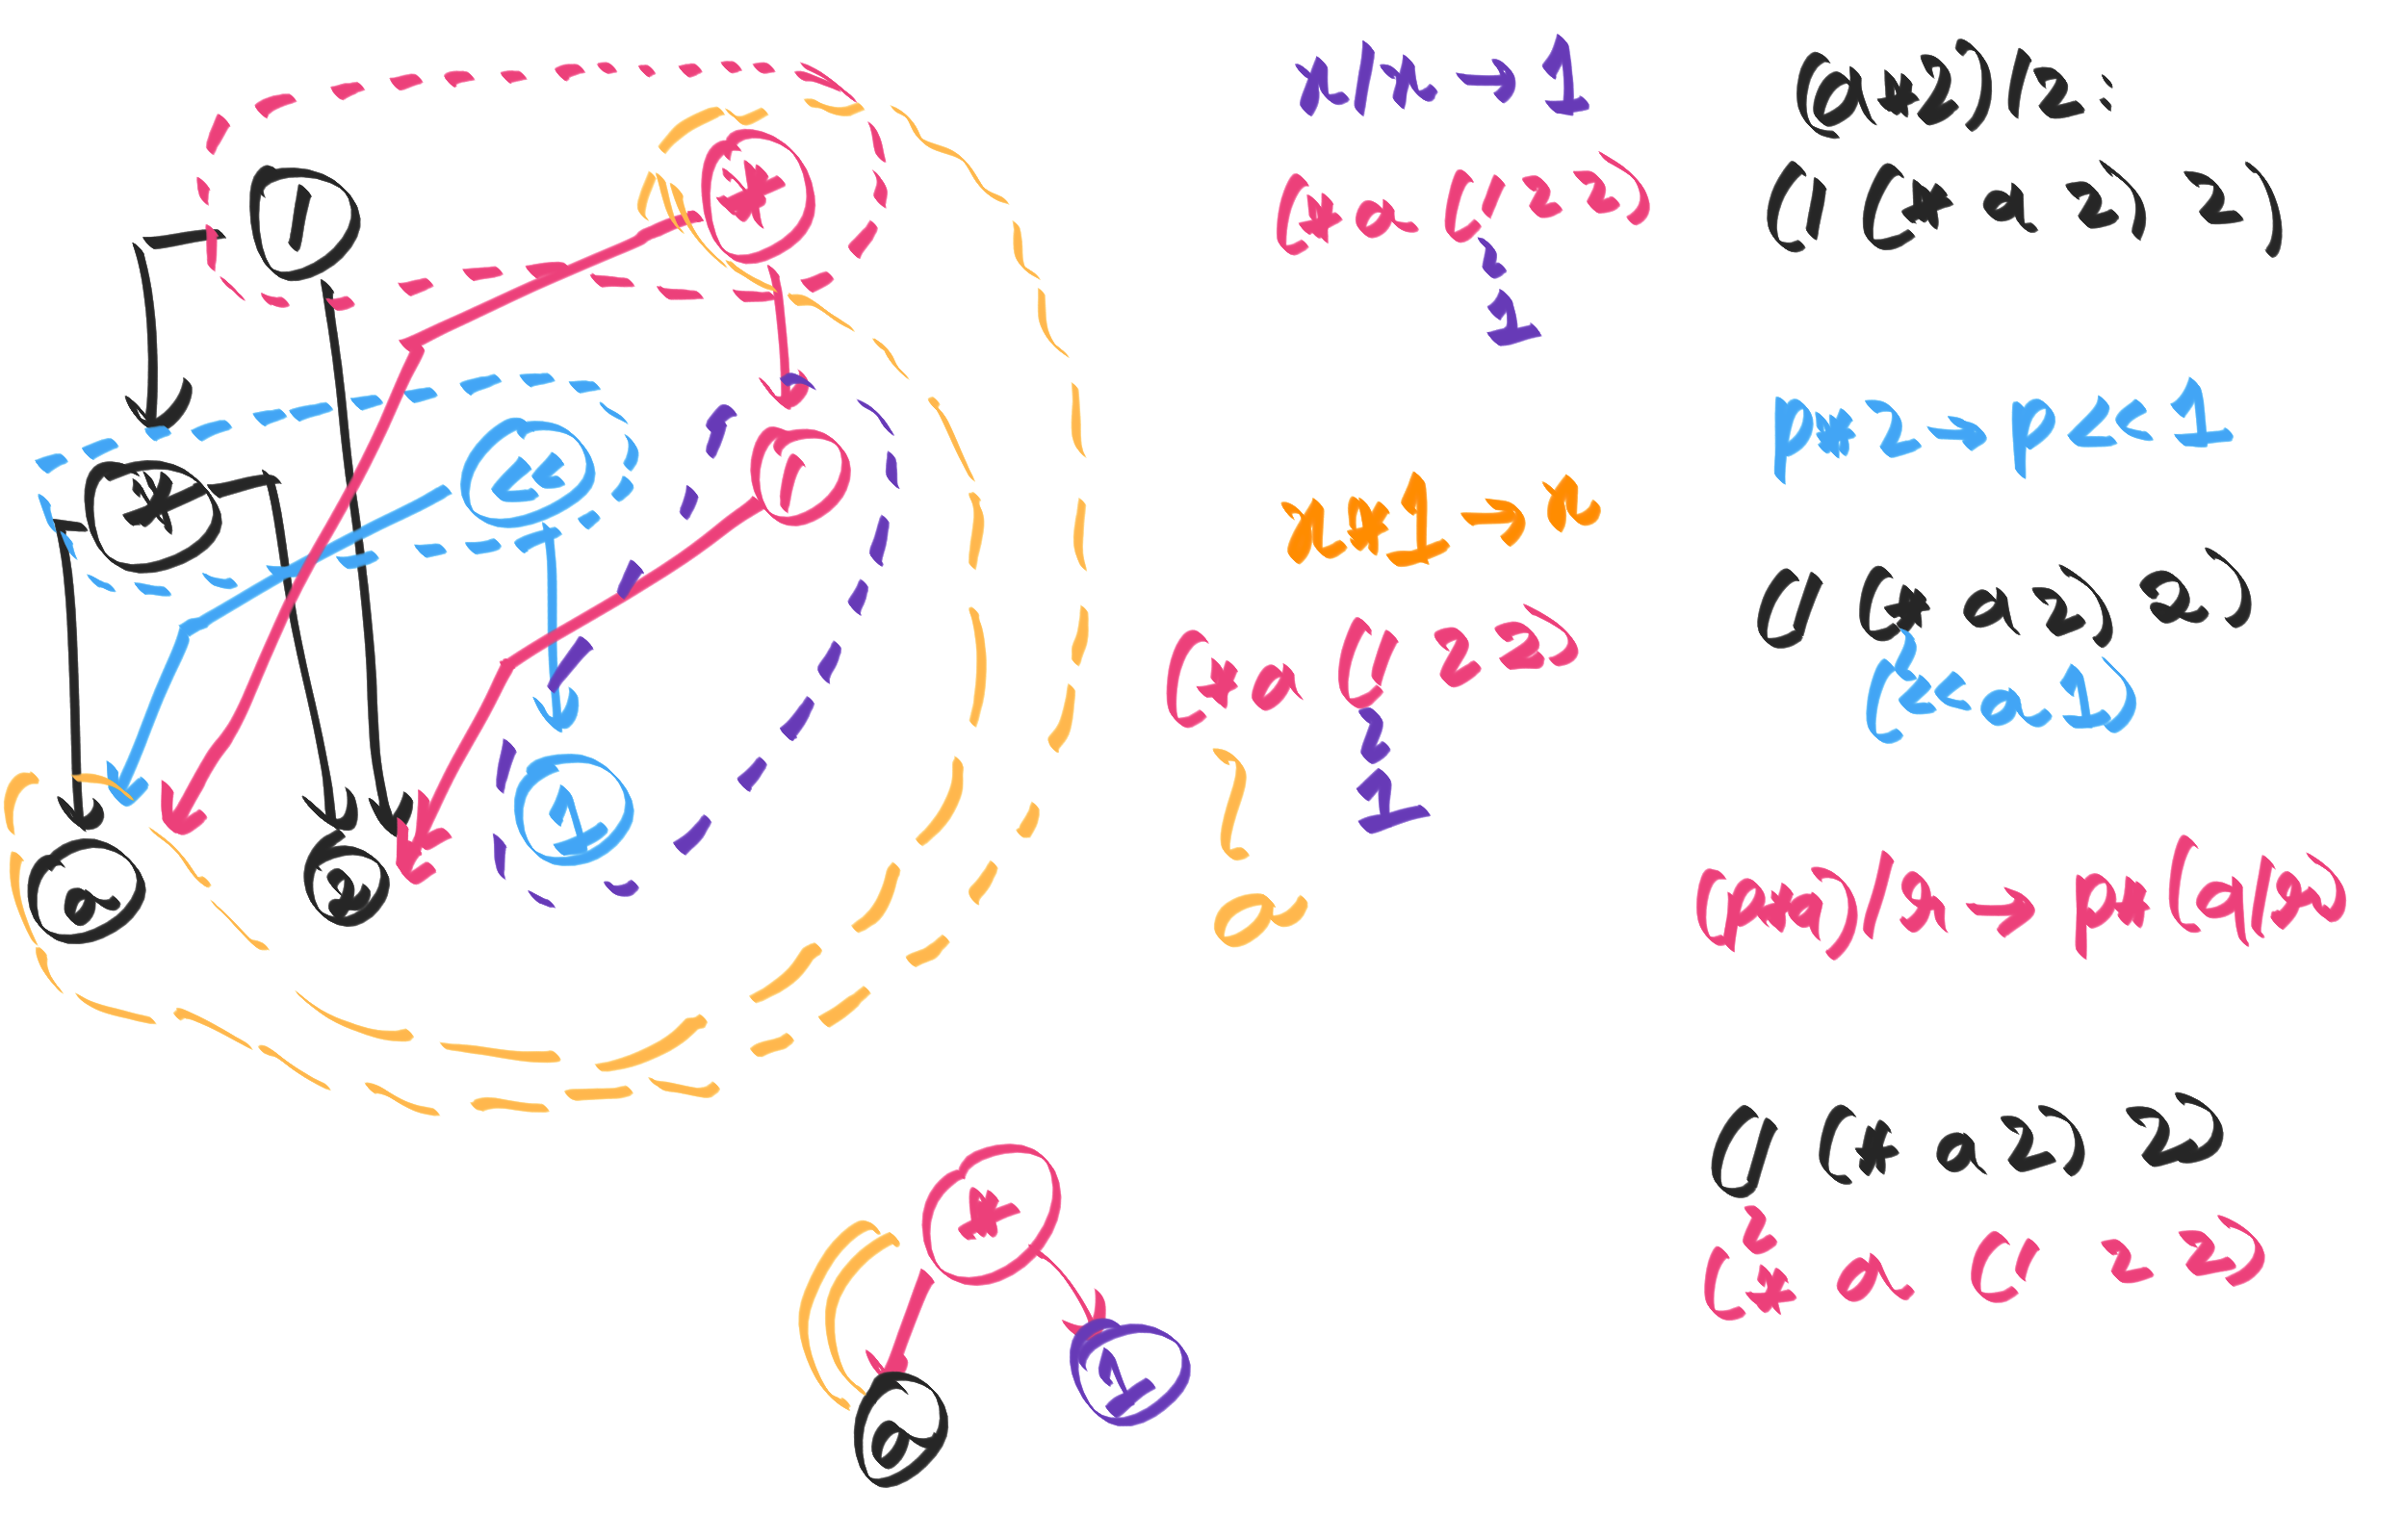
\includegraphics[width=\textwidth]{./eg-1-6.png}
\end{frame}

\begin{frame}[fragile]{\egg: Fast and extensible equality saturation (7)}
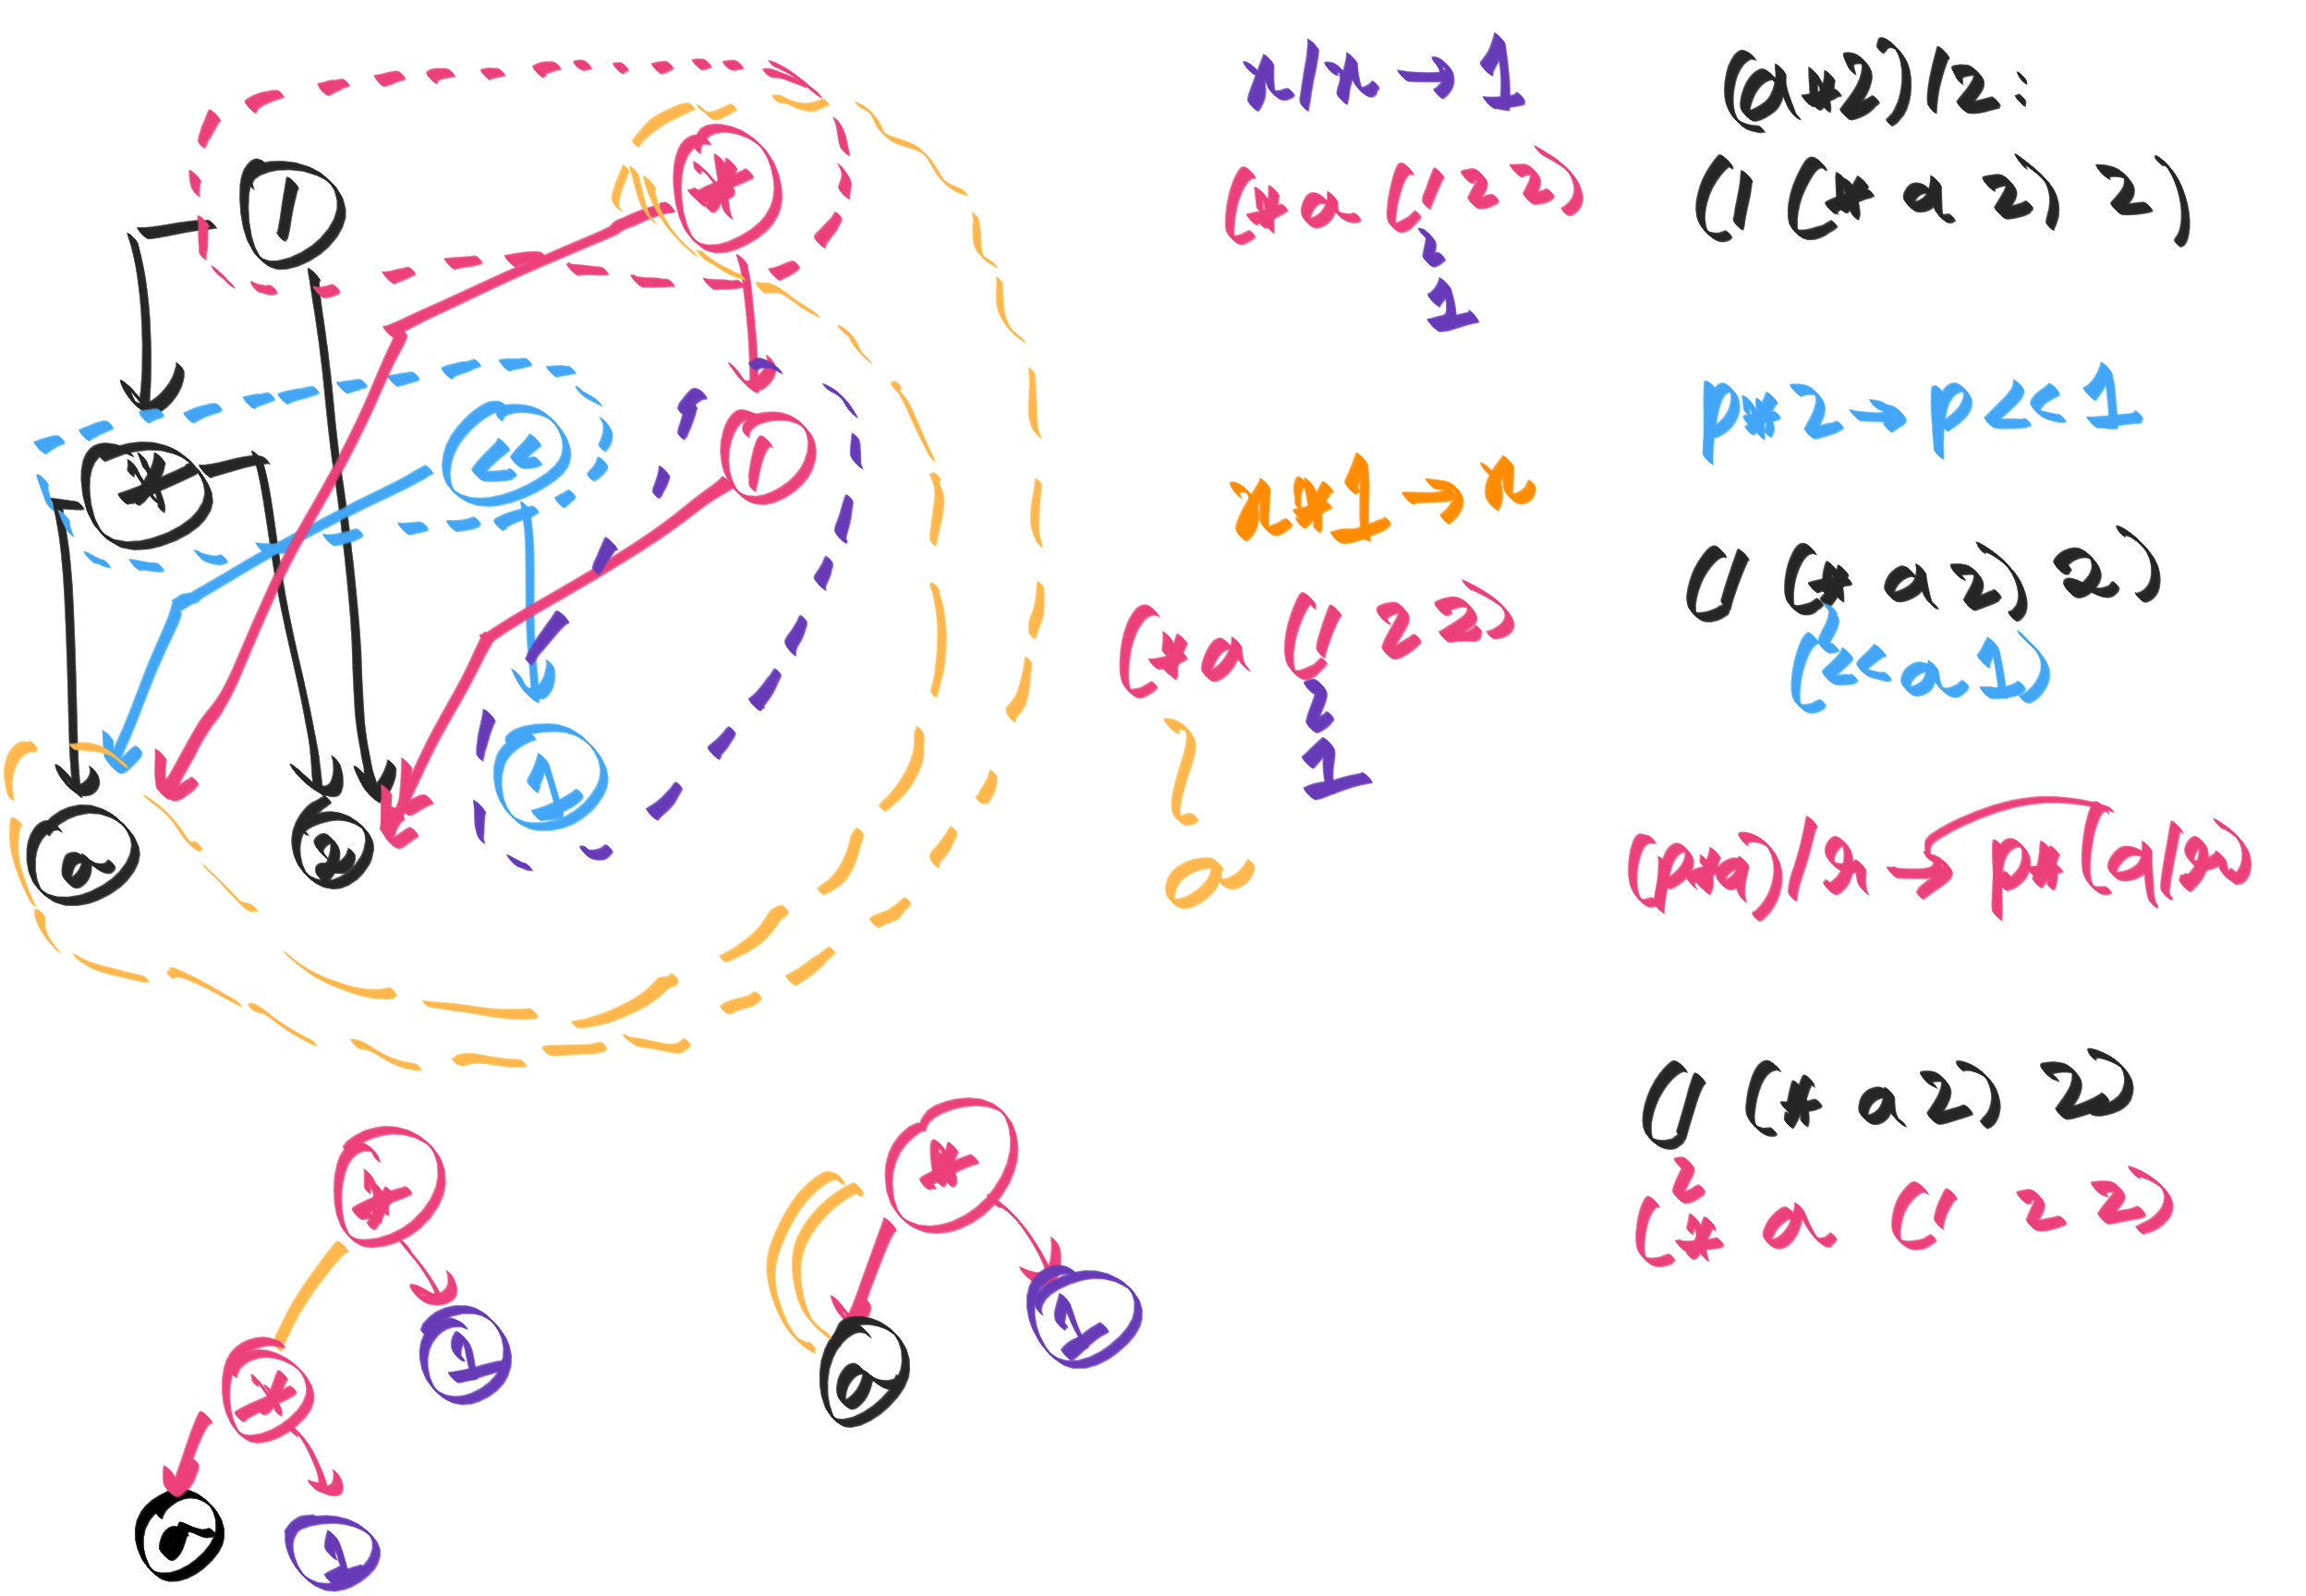
\includegraphics[width=\textwidth]{./eg-1-7.png}
\end{frame}


\begin{frame}[fragile]{\egg: Fast and extensible equality saturation (8)}
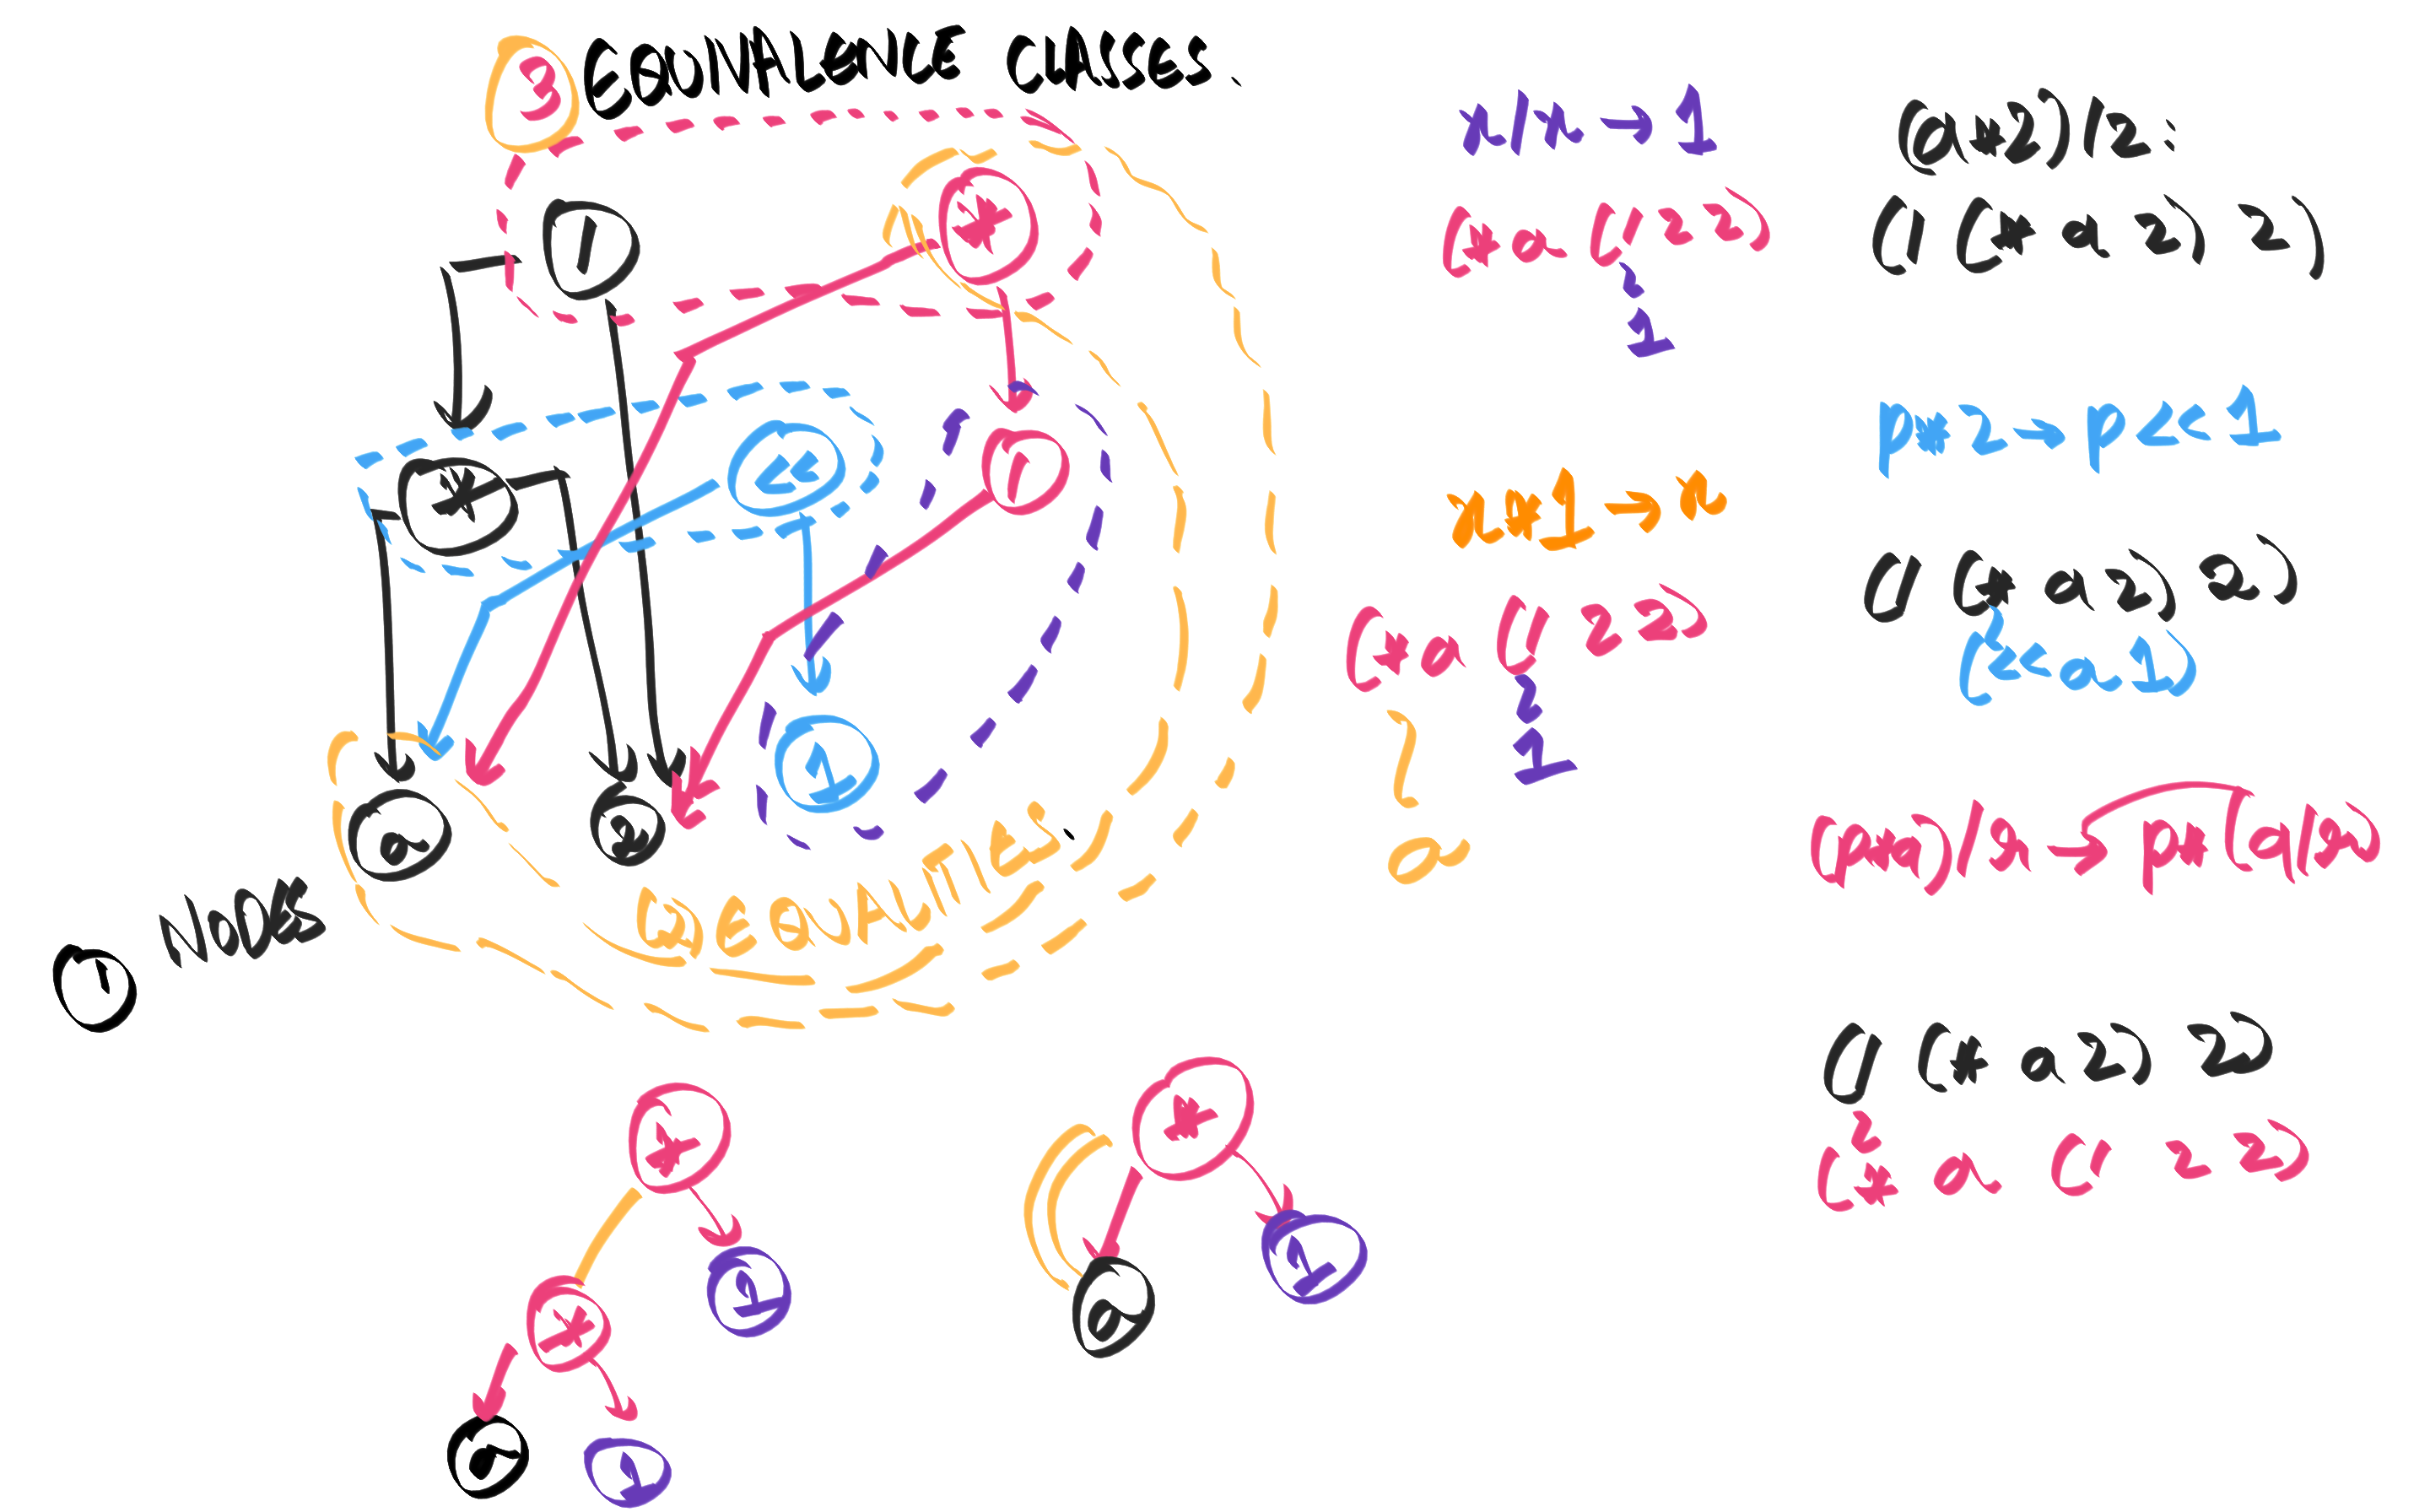
\includegraphics[width=\textwidth]{./eg-1-8.png}
\end{frame}


\begin{frame}{Evaluation: Herbie}
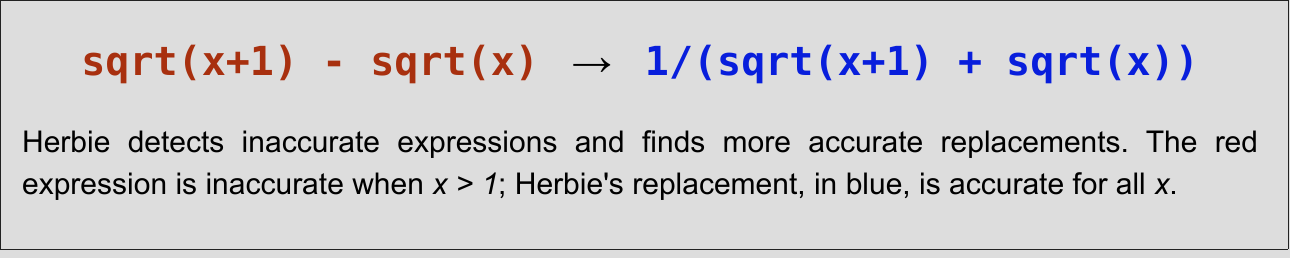
\includegraphics[width=\textwidth]{./herbie-sales-pitch.png}
\pause

$$
\sqrt{x+1}-\sqrt{x} =
\frac{(\sqrt{x+1}-\sqrt{x})(\sqrt{x+1}+\sqrt{x})}{\sqrt{x+1}+\sqrt{x}}
= \frac{(x+1)-x}{\sqrt{x+1}+\sqrt{x}} = \frac{1}{(\sqrt{x+1}+\sqrt{x})}
$$
\pause
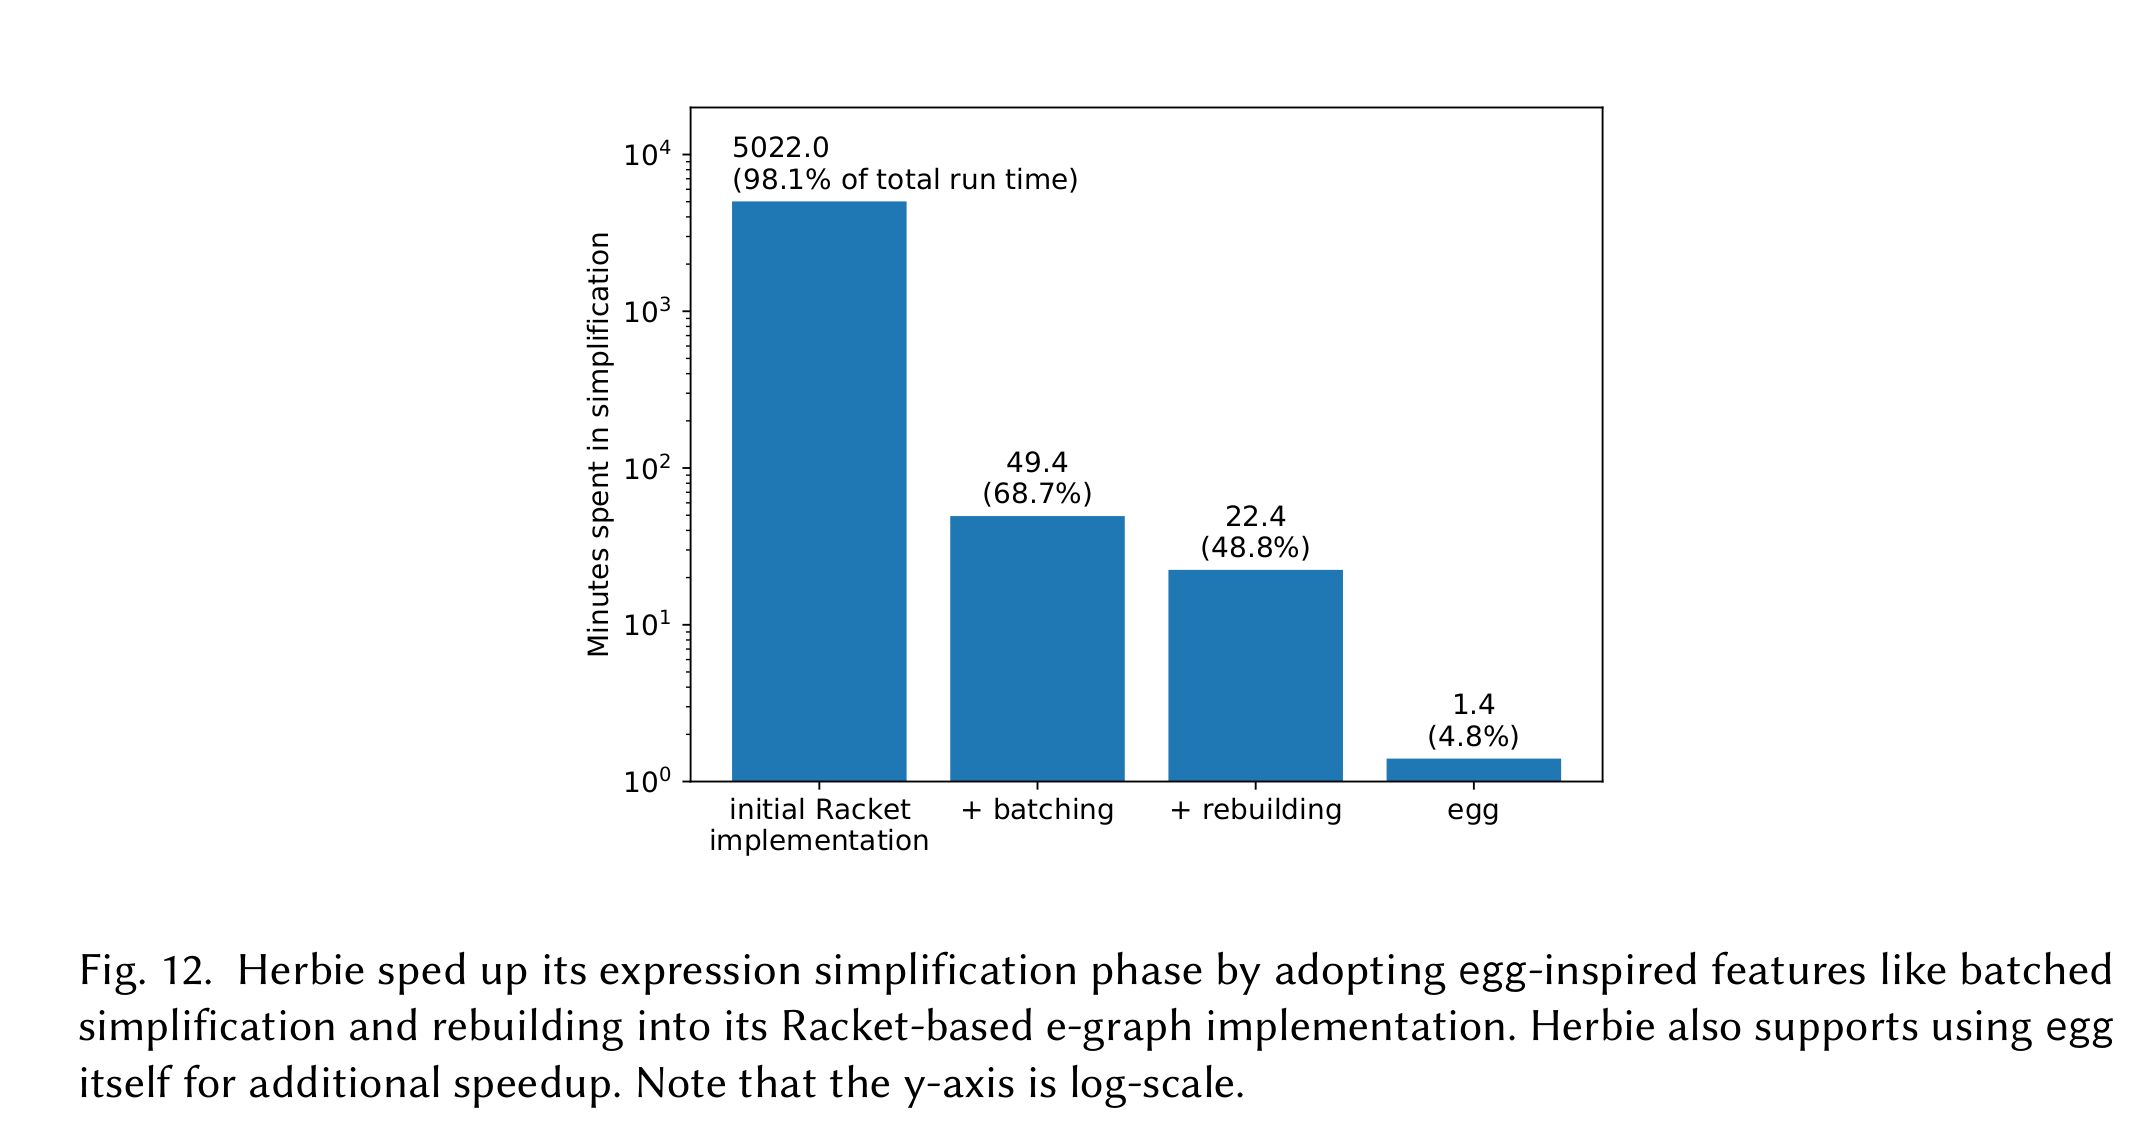
\includegraphics[width=0.8\textwidth]{./herbie-speedup.png}

\end{frame}

\begin{frame}[fragile]{Herbie: Using \egg --- Analysis and rewrite}
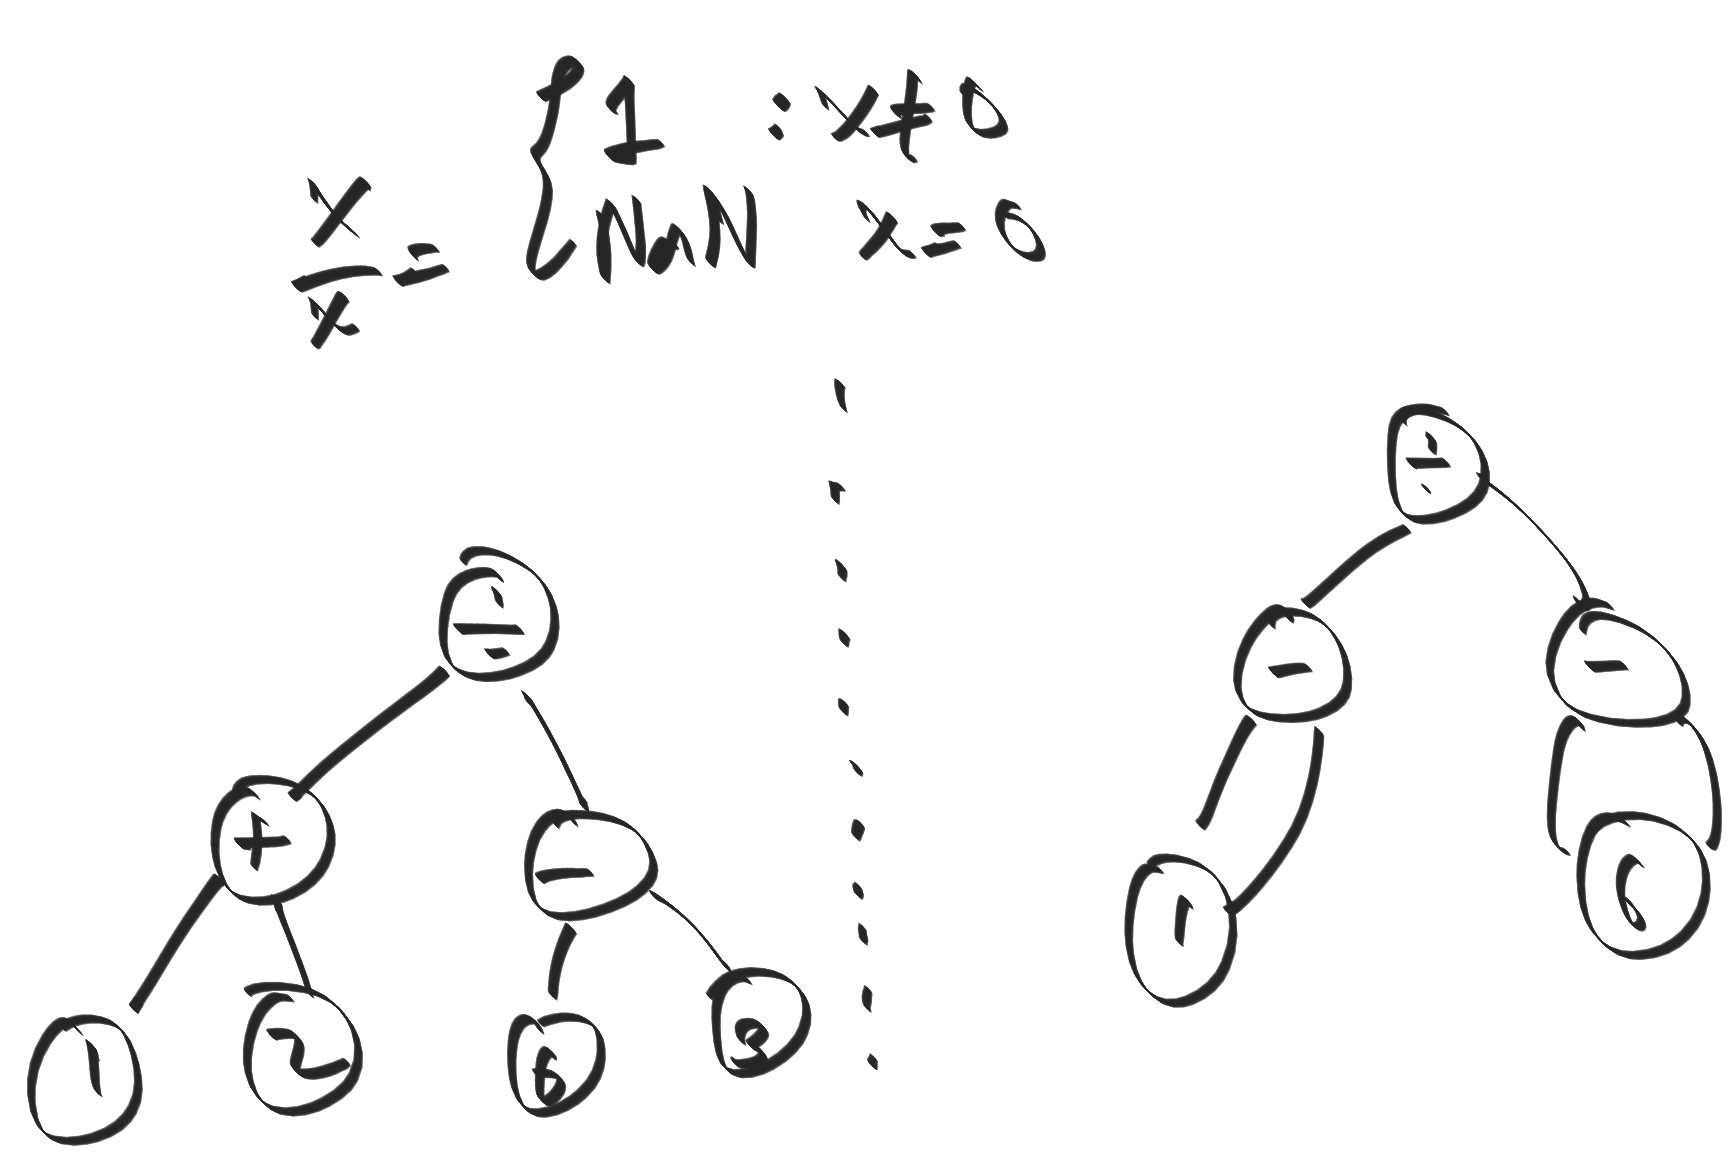
\includegraphics[width=\textwidth]{./rewrite-1.png}
\end{frame}


\begin{frame}[fragile]{Herbie: Using \egg --- Analysis and rewrite}
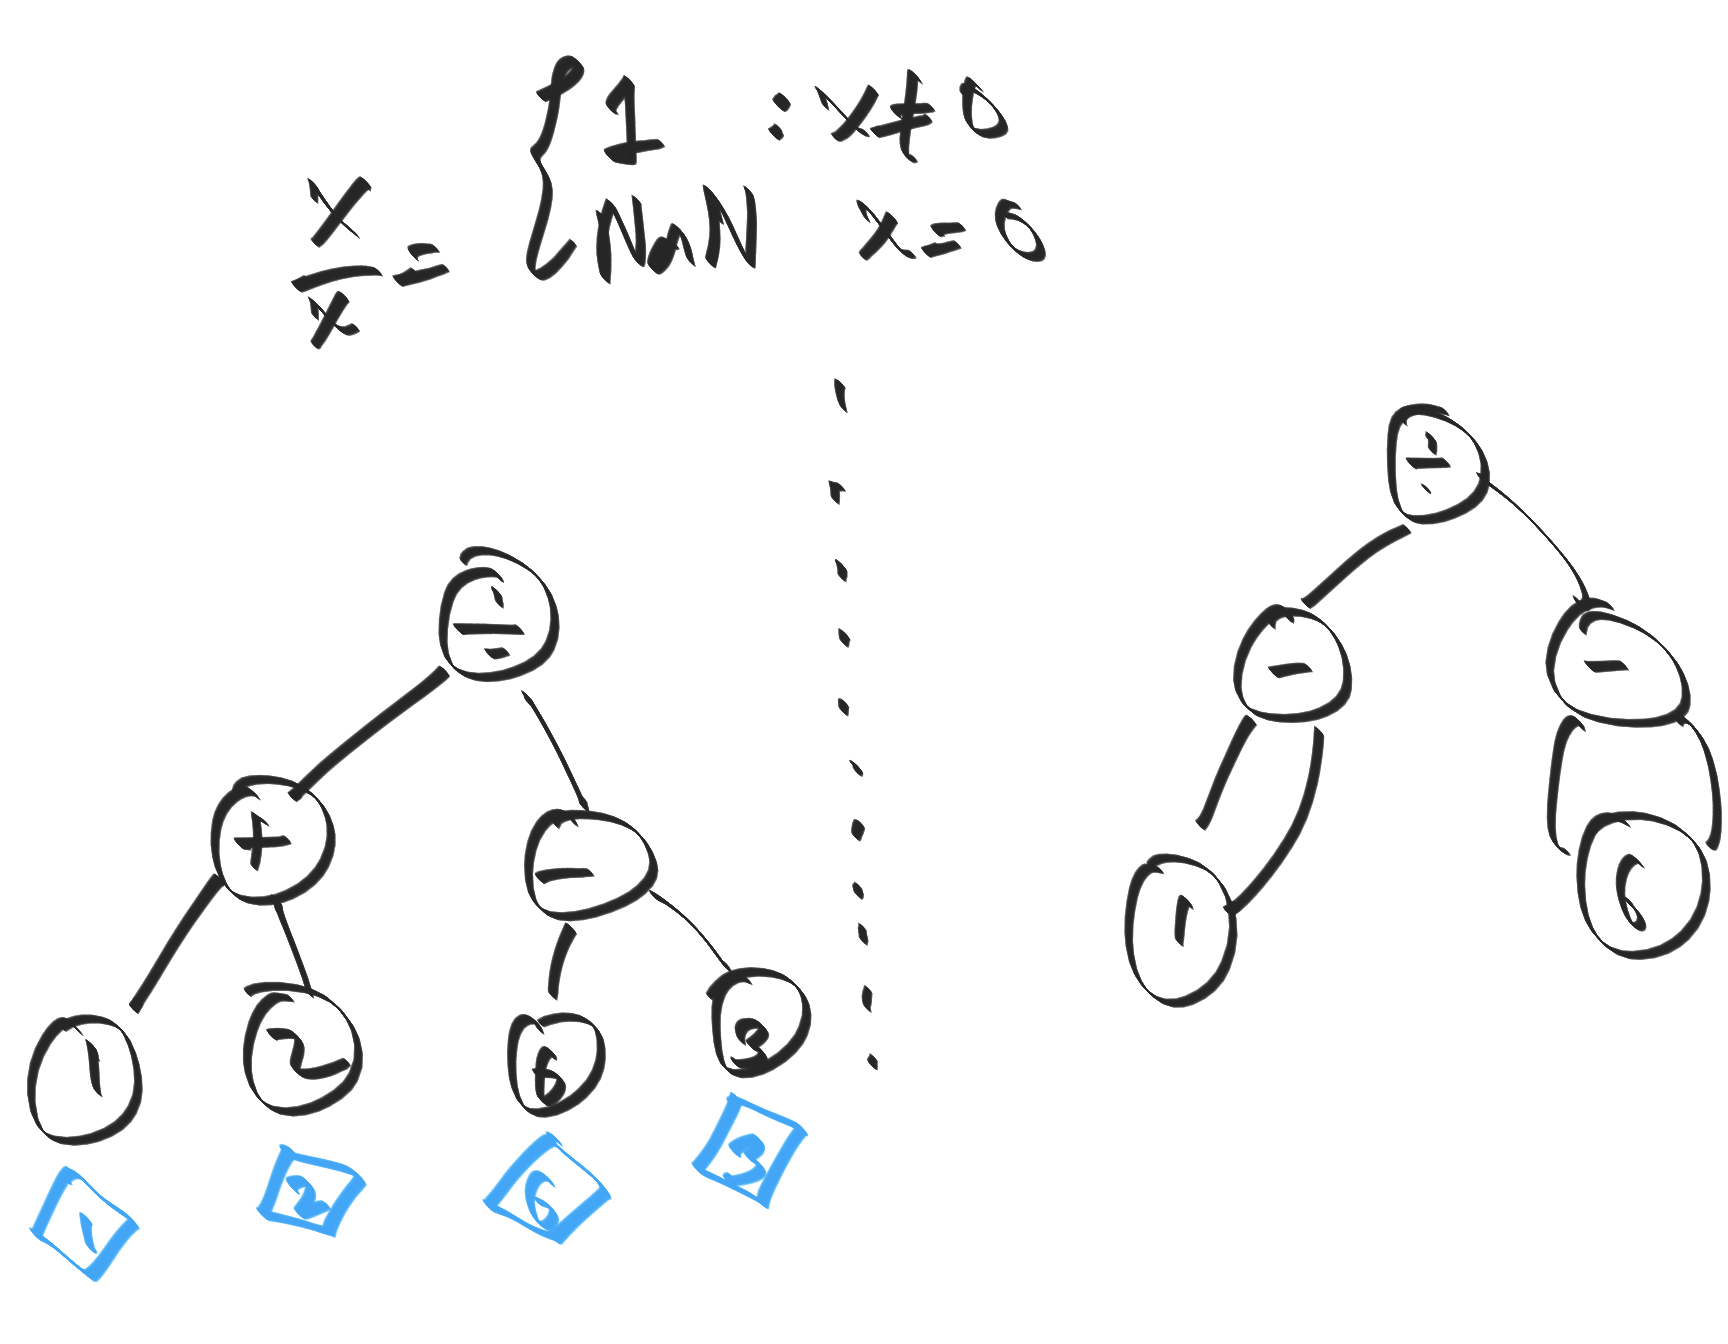
\includegraphics[width=\textwidth]{./rewrite-2.png}
\end{frame}


\begin{frame}[fragile]{Herbie: Using \egg --- Analysis and rewrite}
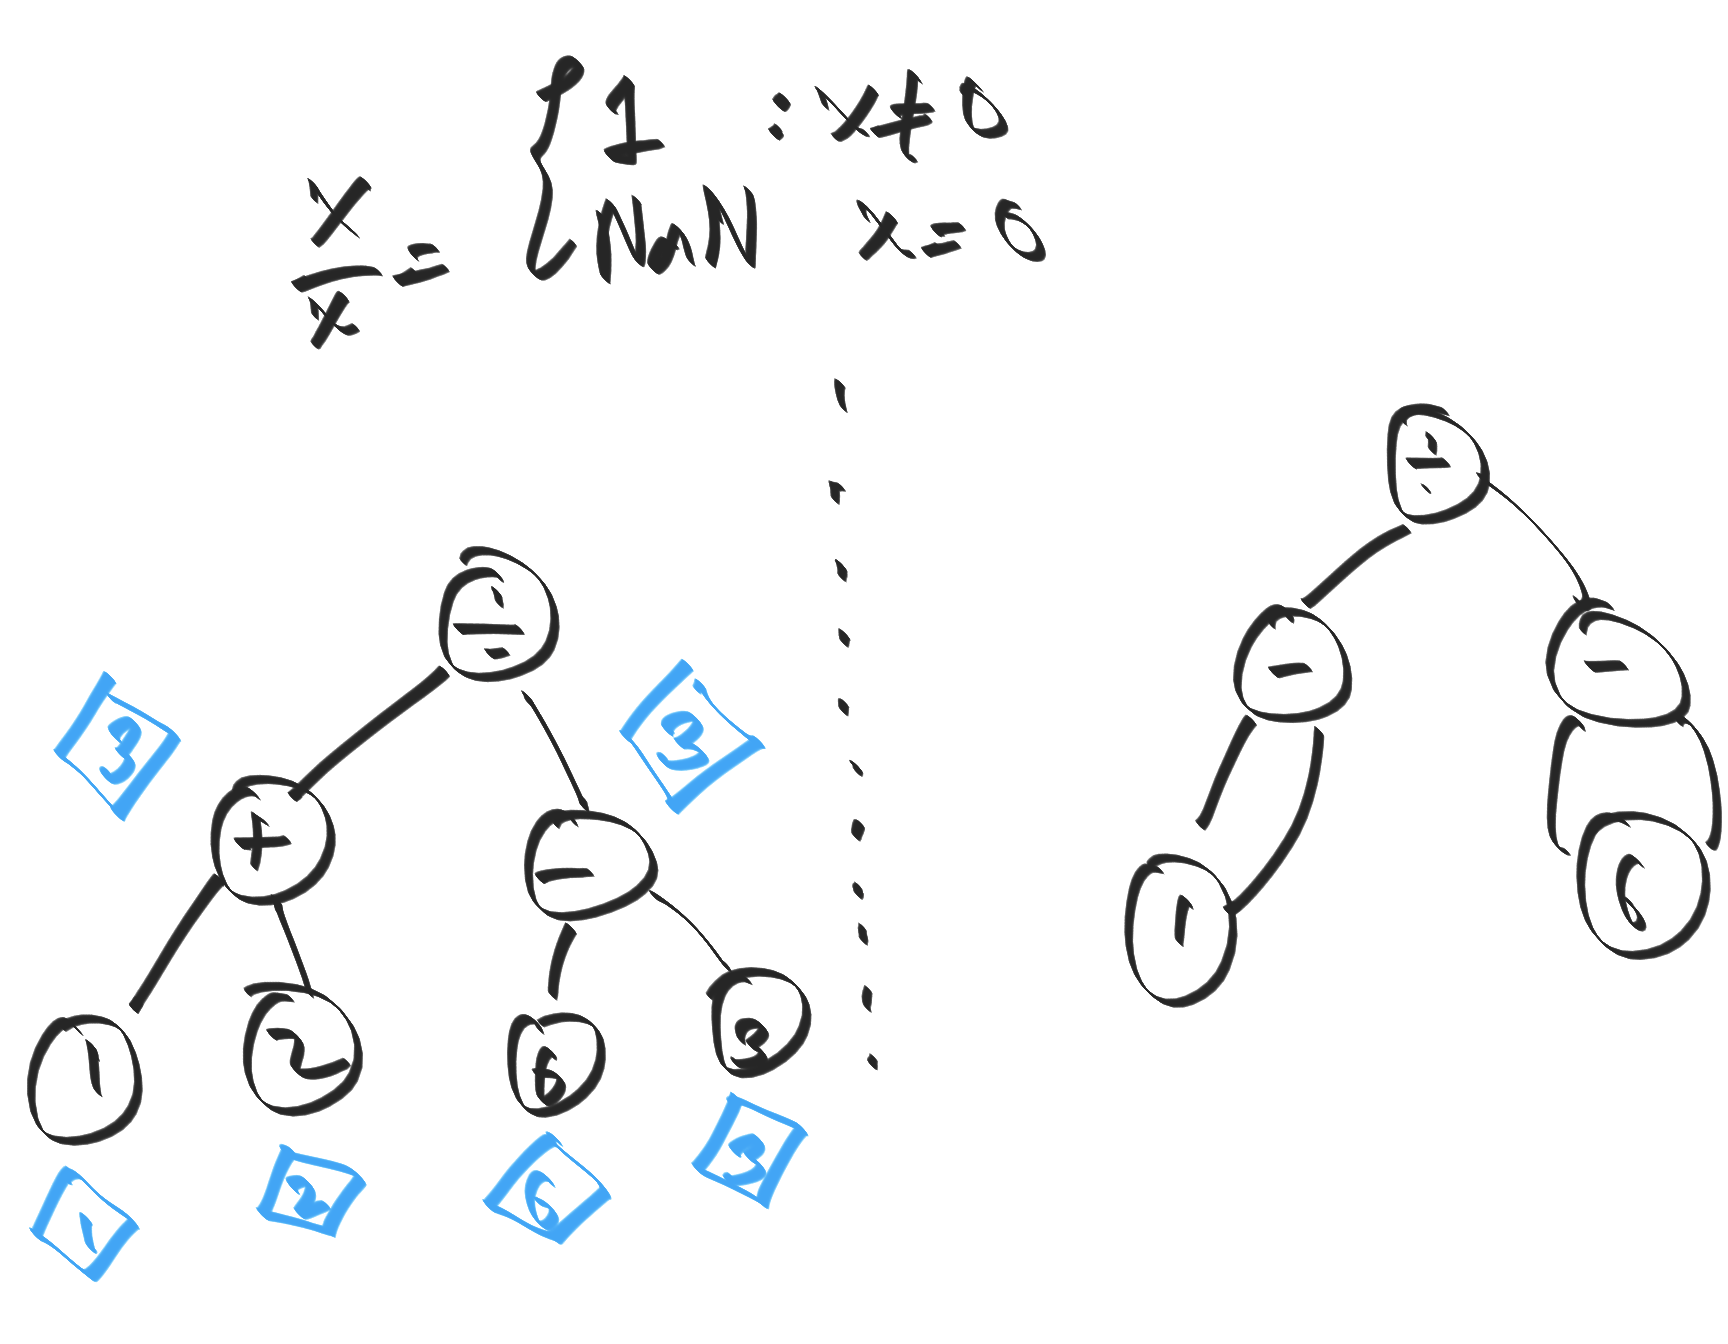
\includegraphics[width=\textwidth]{./rewrite-3.png}
\end{frame}


\begin{frame}[fragile]{Herbie: Using \egg --- Analysis and rewrite}
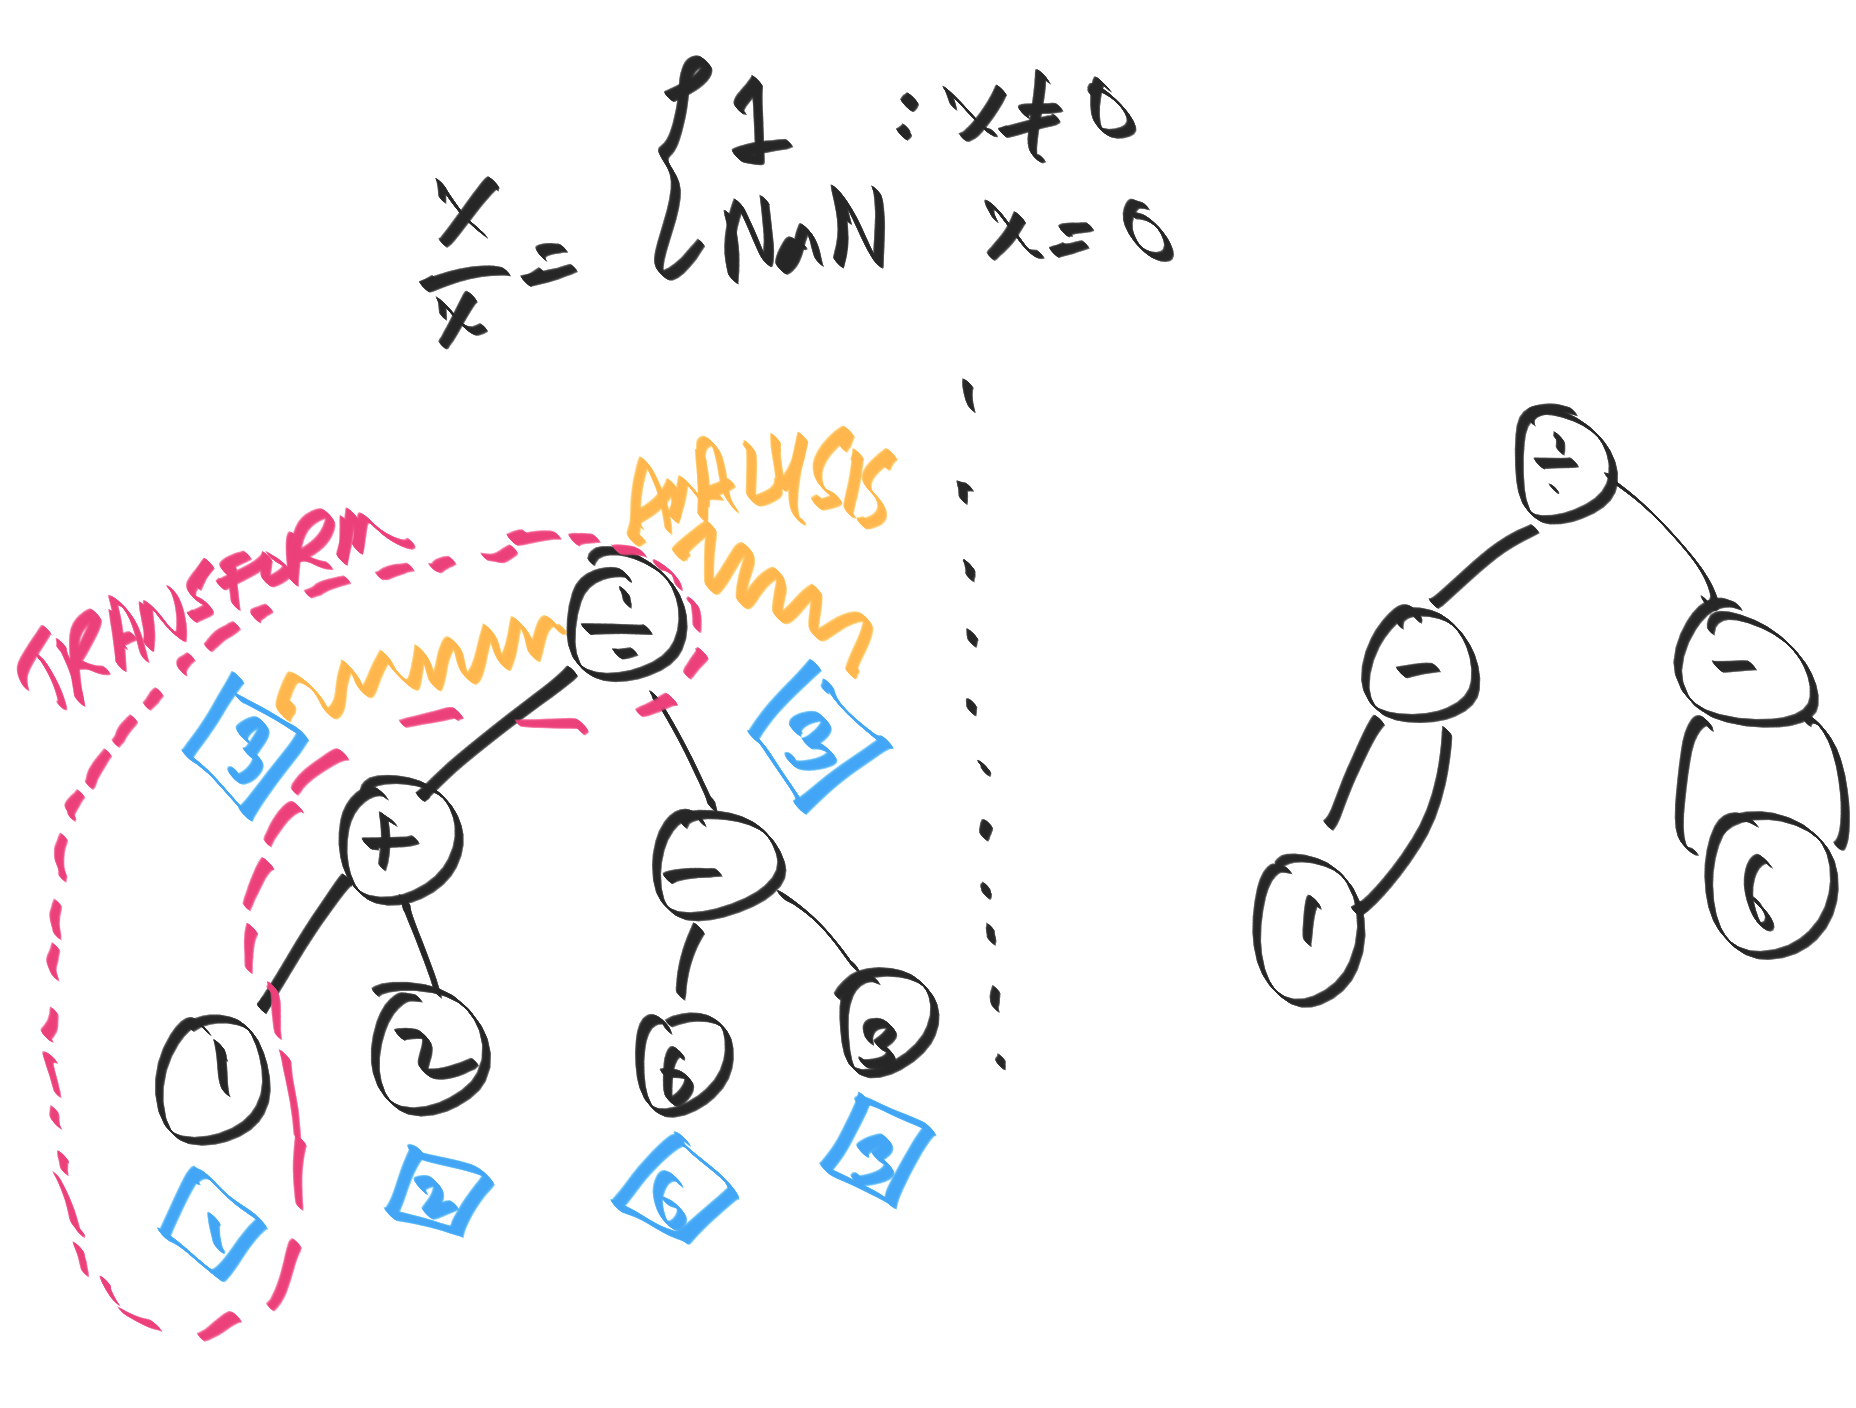
\includegraphics[width=\textwidth]{./rewrite-4.png}
\end{frame}


\begin{frame}[fragile]{Herbie: Using \egg --- Analysis and rewrite}
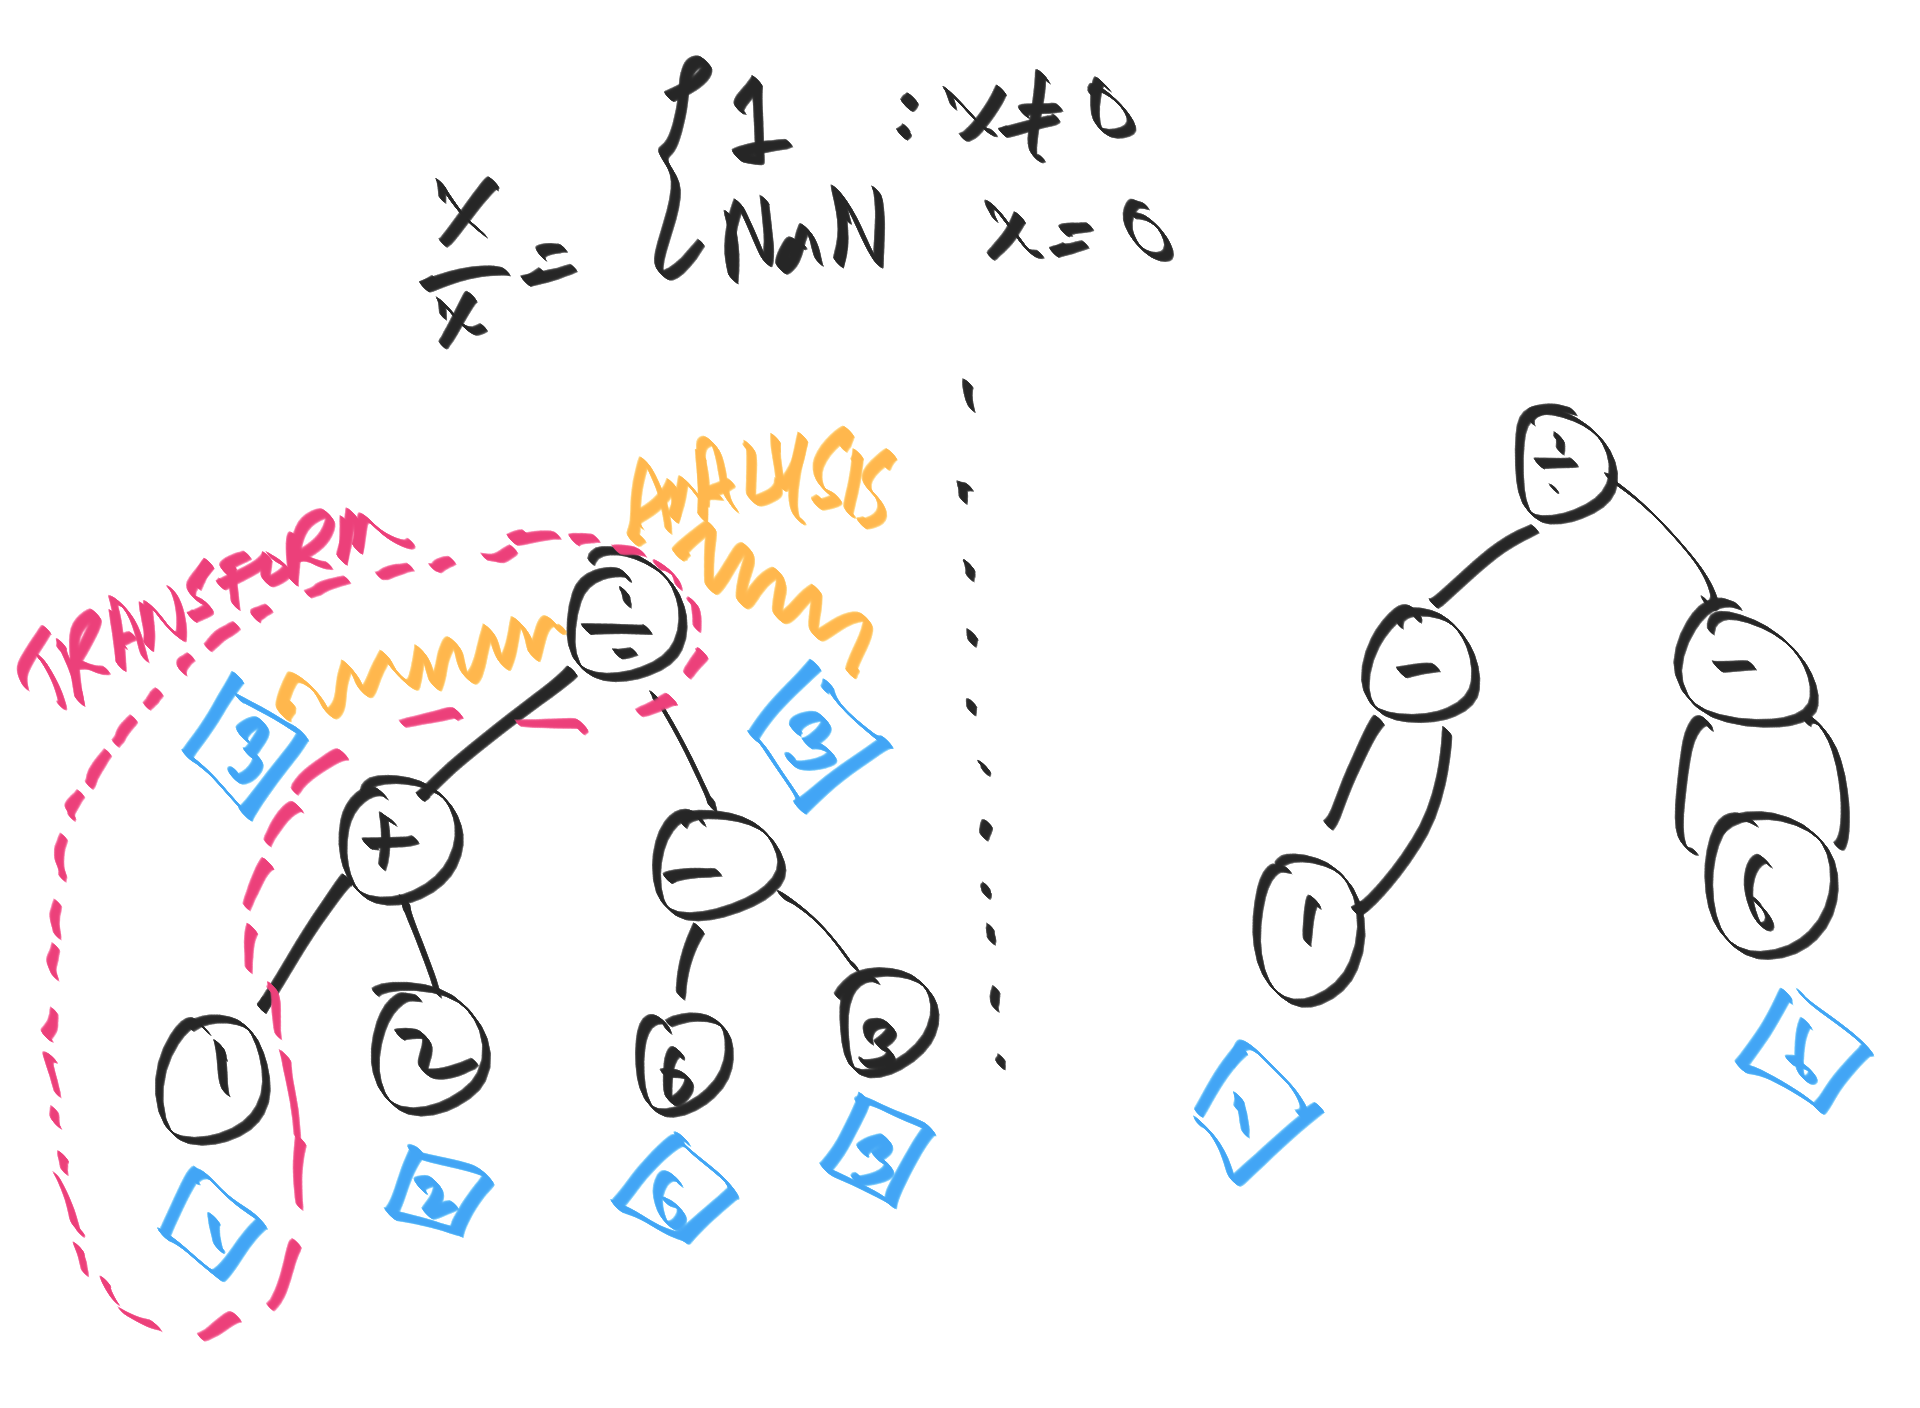
\includegraphics[width=\textwidth]{./rewrite-5.png}
\end{frame}


\begin{frame}[fragile]{Herbie: Using \egg --- Analysis and rewrite}
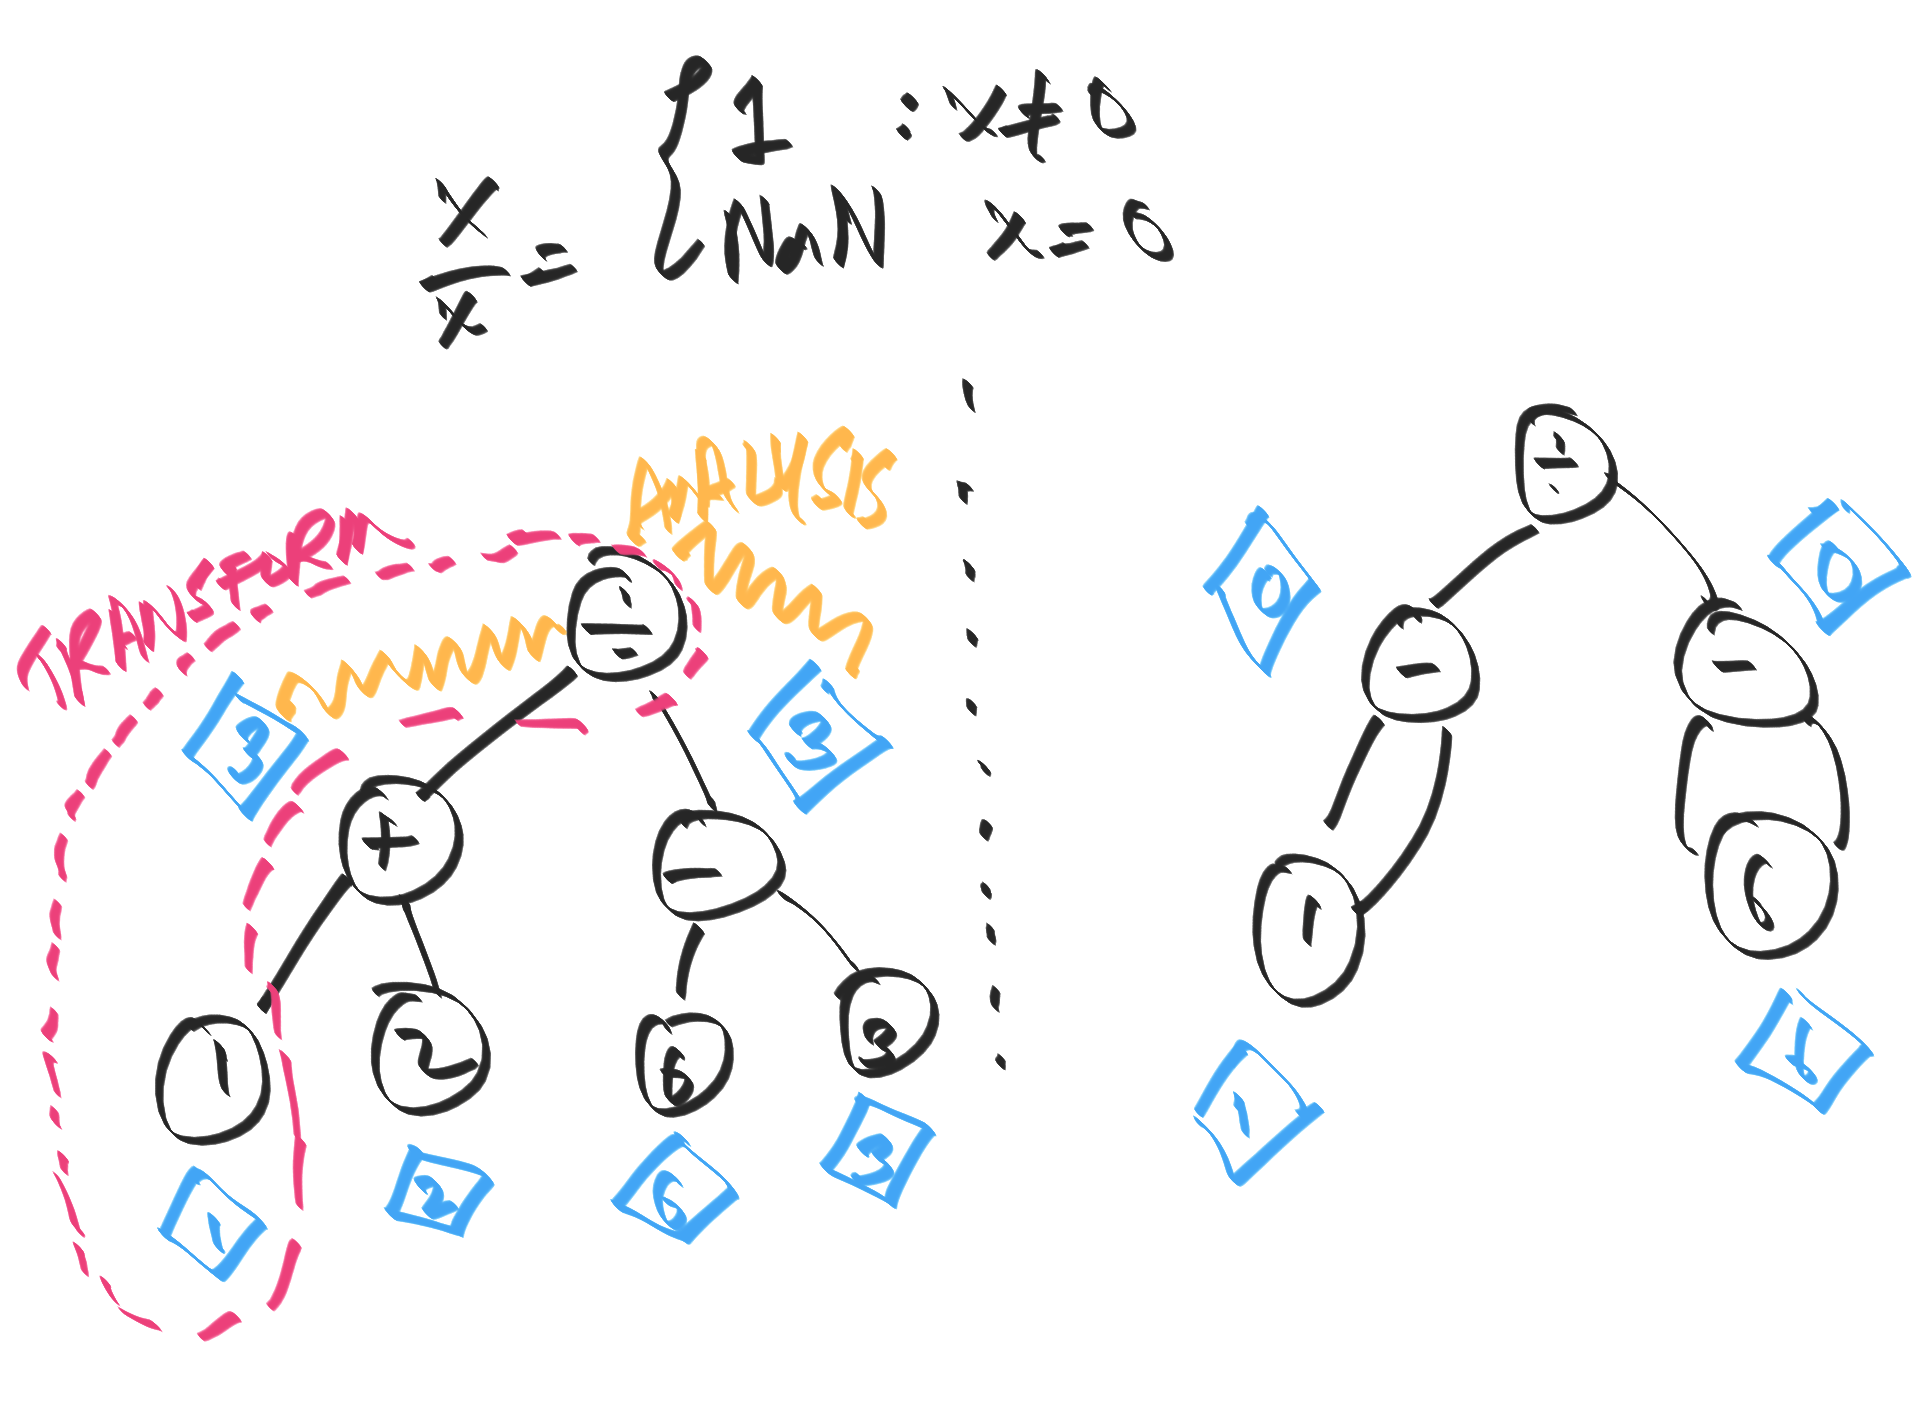
\includegraphics[width=\textwidth]{./rewrite-6.png}
\end{frame}


\begin{frame}[fragile]{Herbie: Using \egg --- Analysis and rewrite}
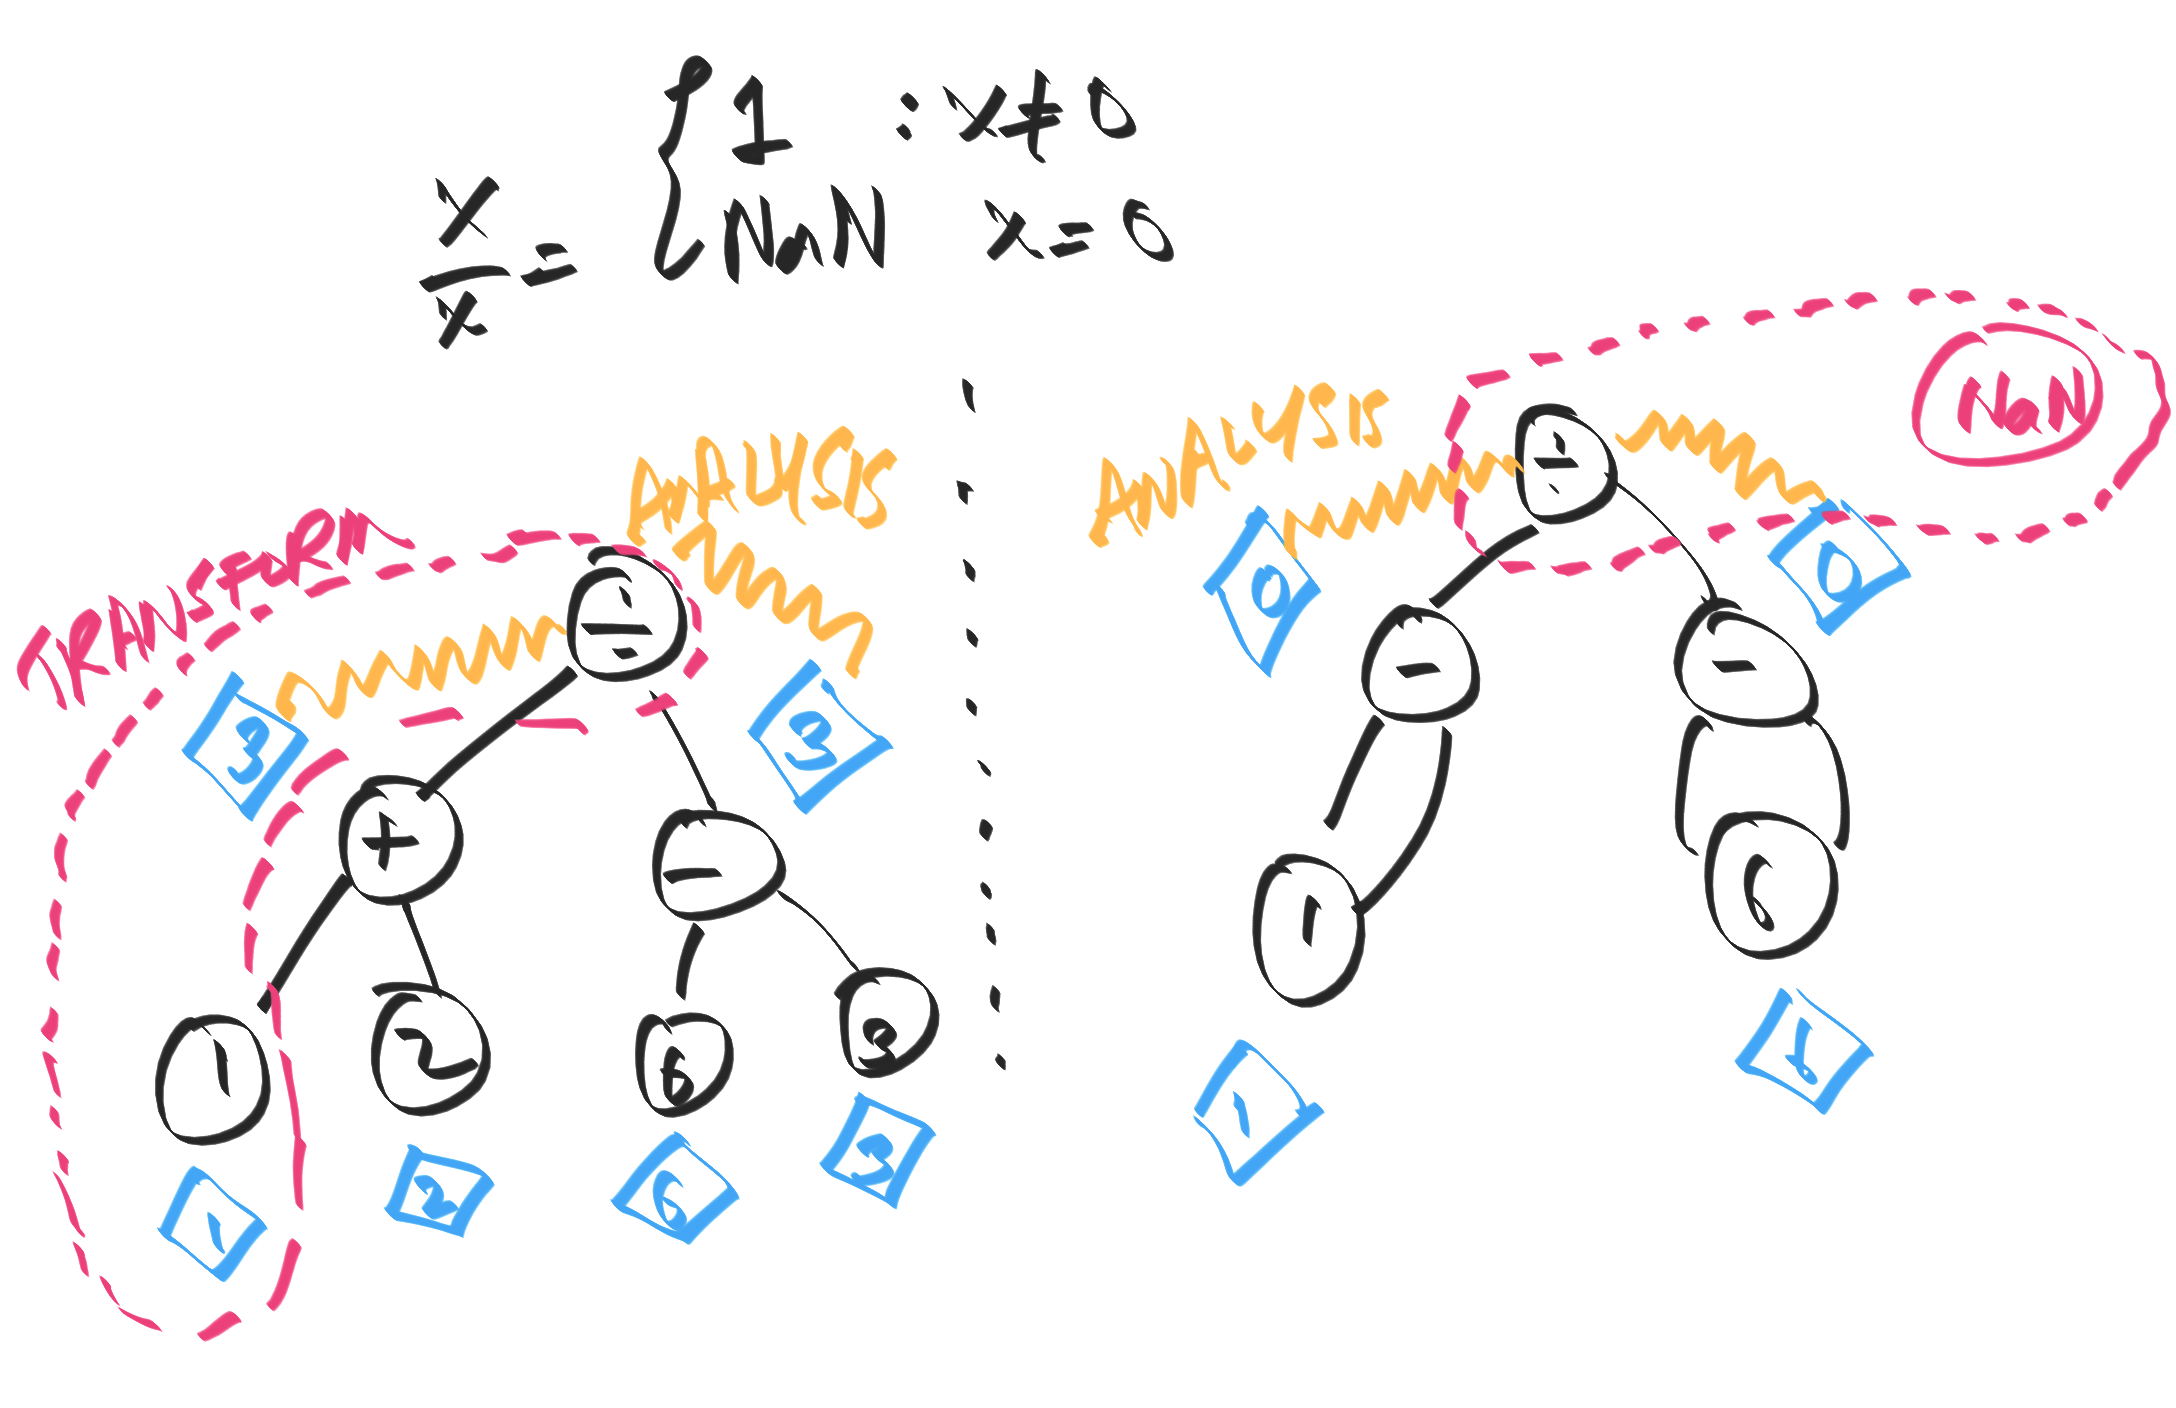
\includegraphics[width=\textwidth]{./rewrite-7.png}
\end{frame}




\begin{frame}[fragile]{Speedup over prior art: Merging}
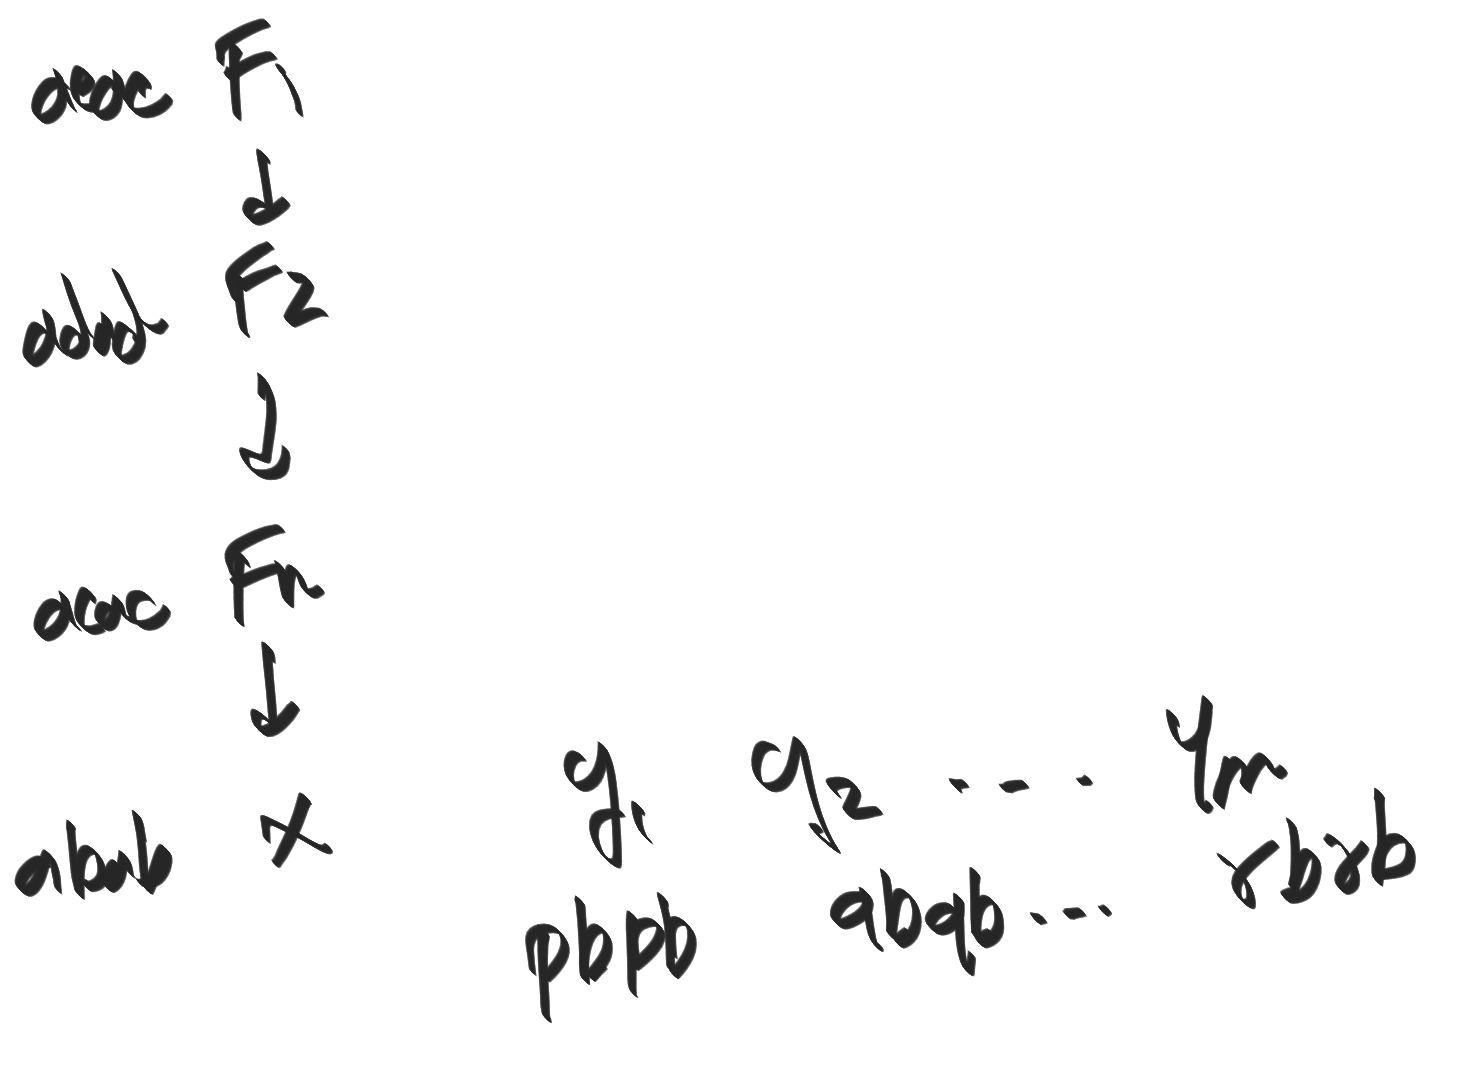
\includegraphics[width=\textwidth]{./eg-2-1.png}
\end{frame}

\begin{frame}[fragile]{Speedup over prior art: Merging}
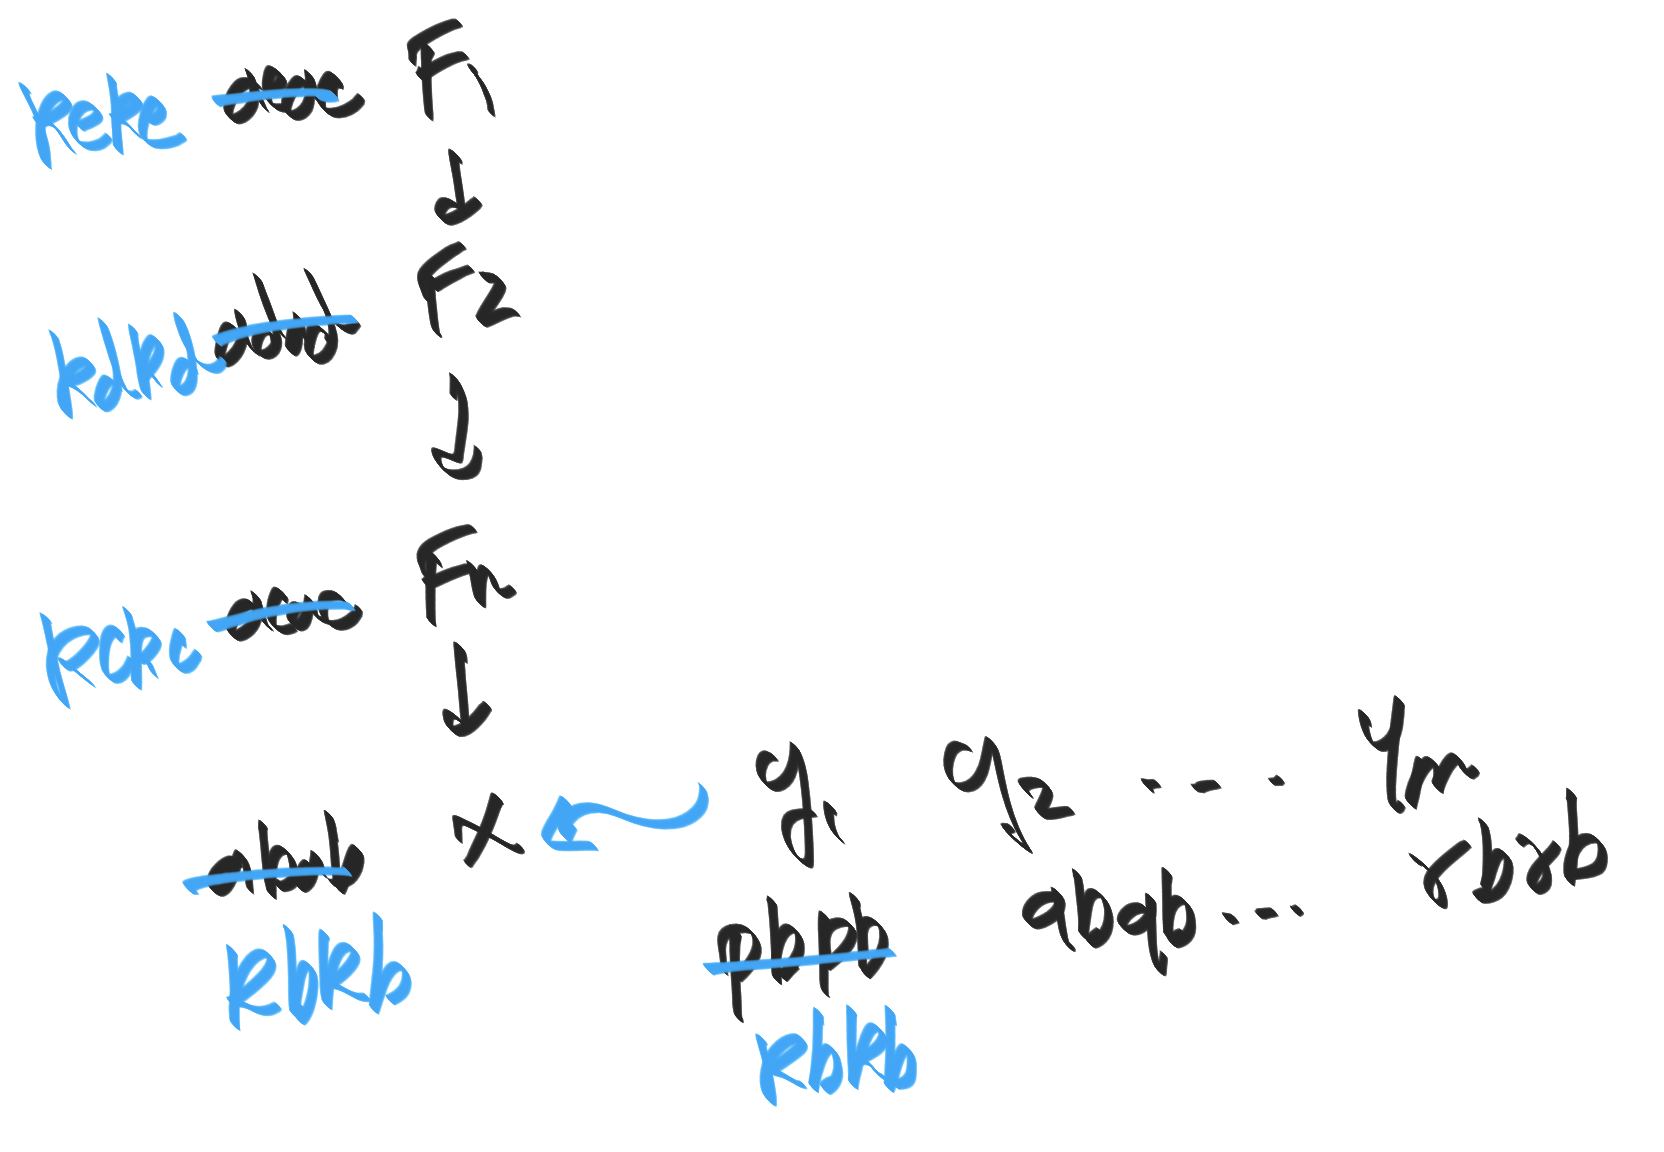
\includegraphics[width=\textwidth]{./eg-2-2.png}
\end{frame}

\begin{frame}[fragile]{Speedup over prior art: Merging}
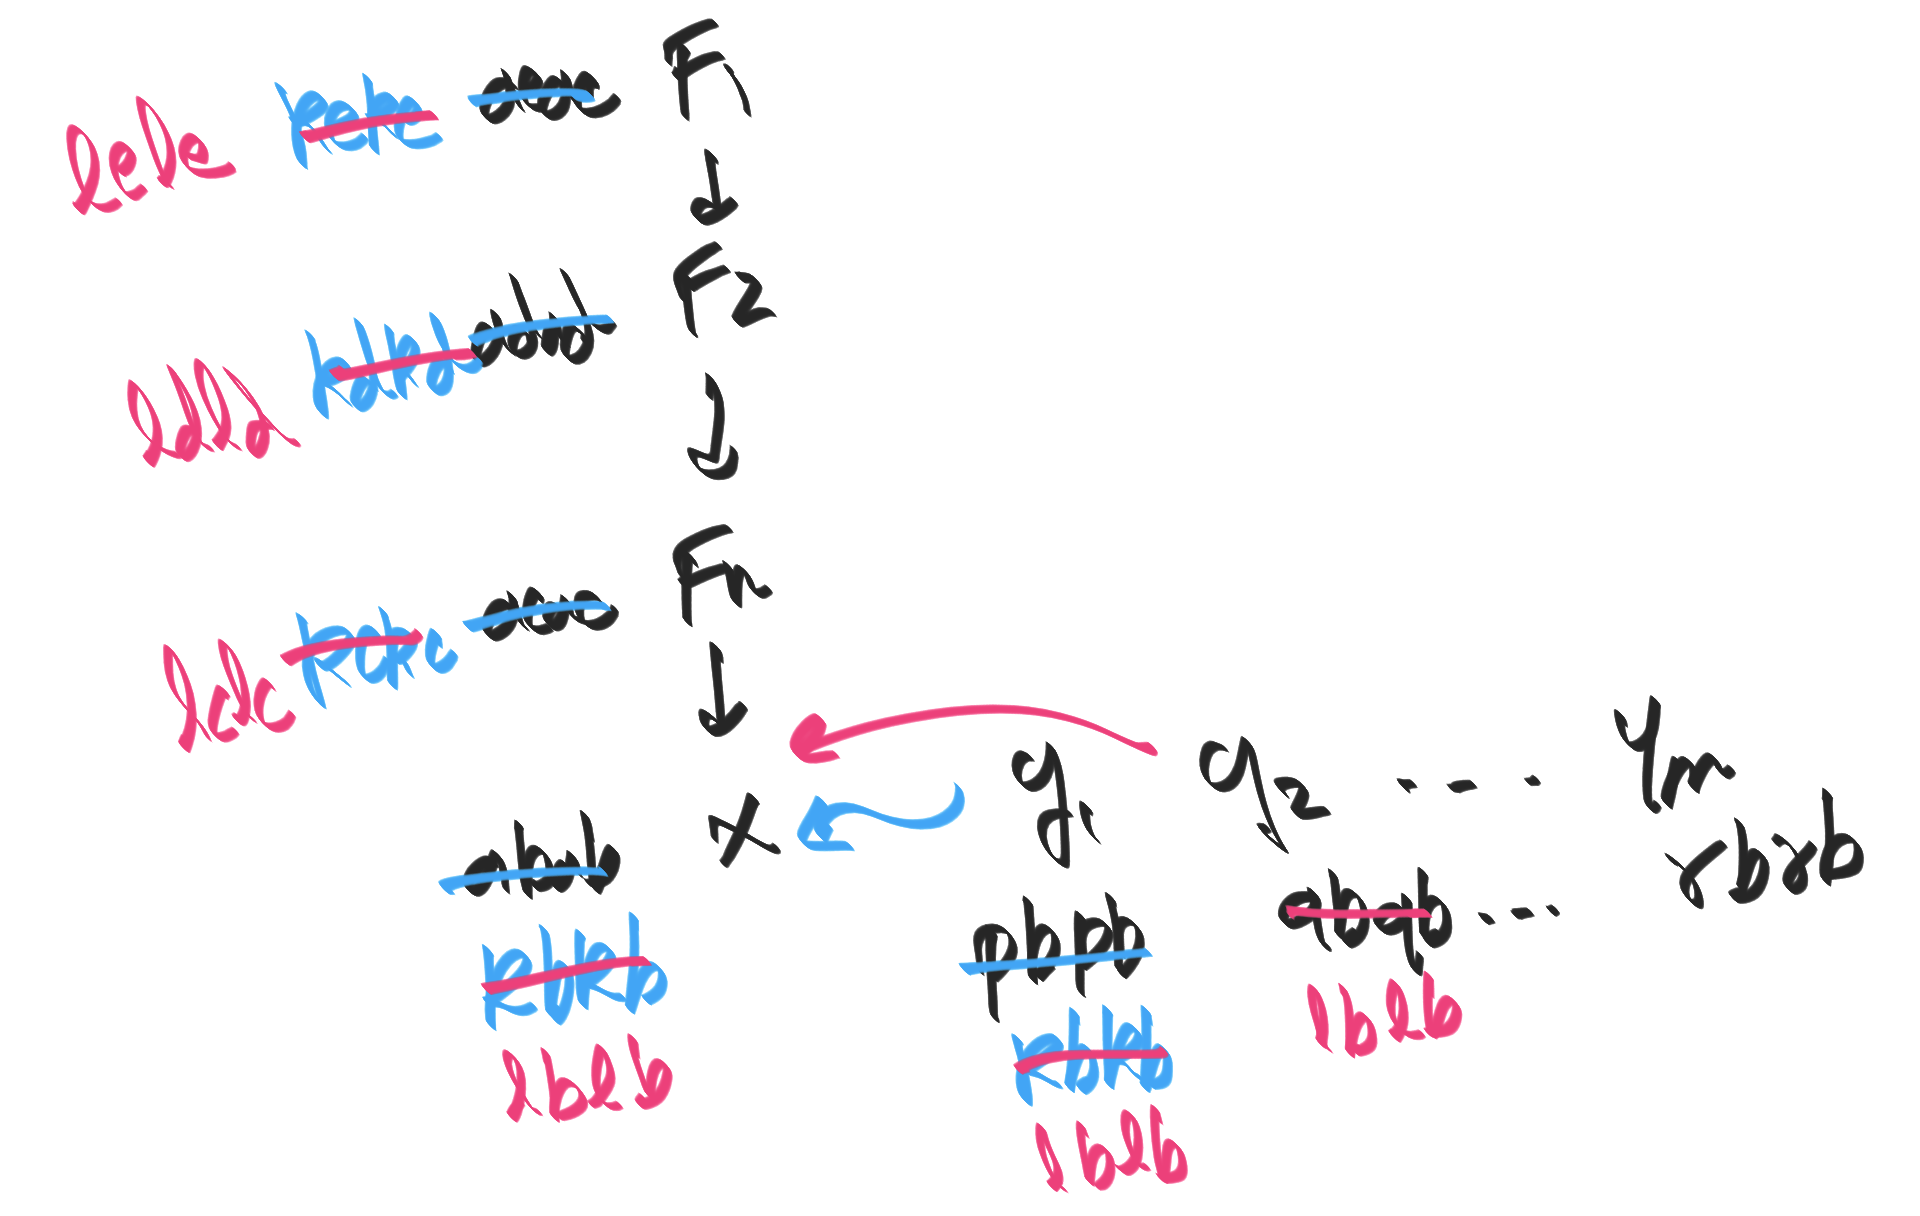
\includegraphics[width=\textwidth]{./eg-2-3.png}
\end{frame}

\begin{frame}[fragile]{Speedup over prior art: Merging}
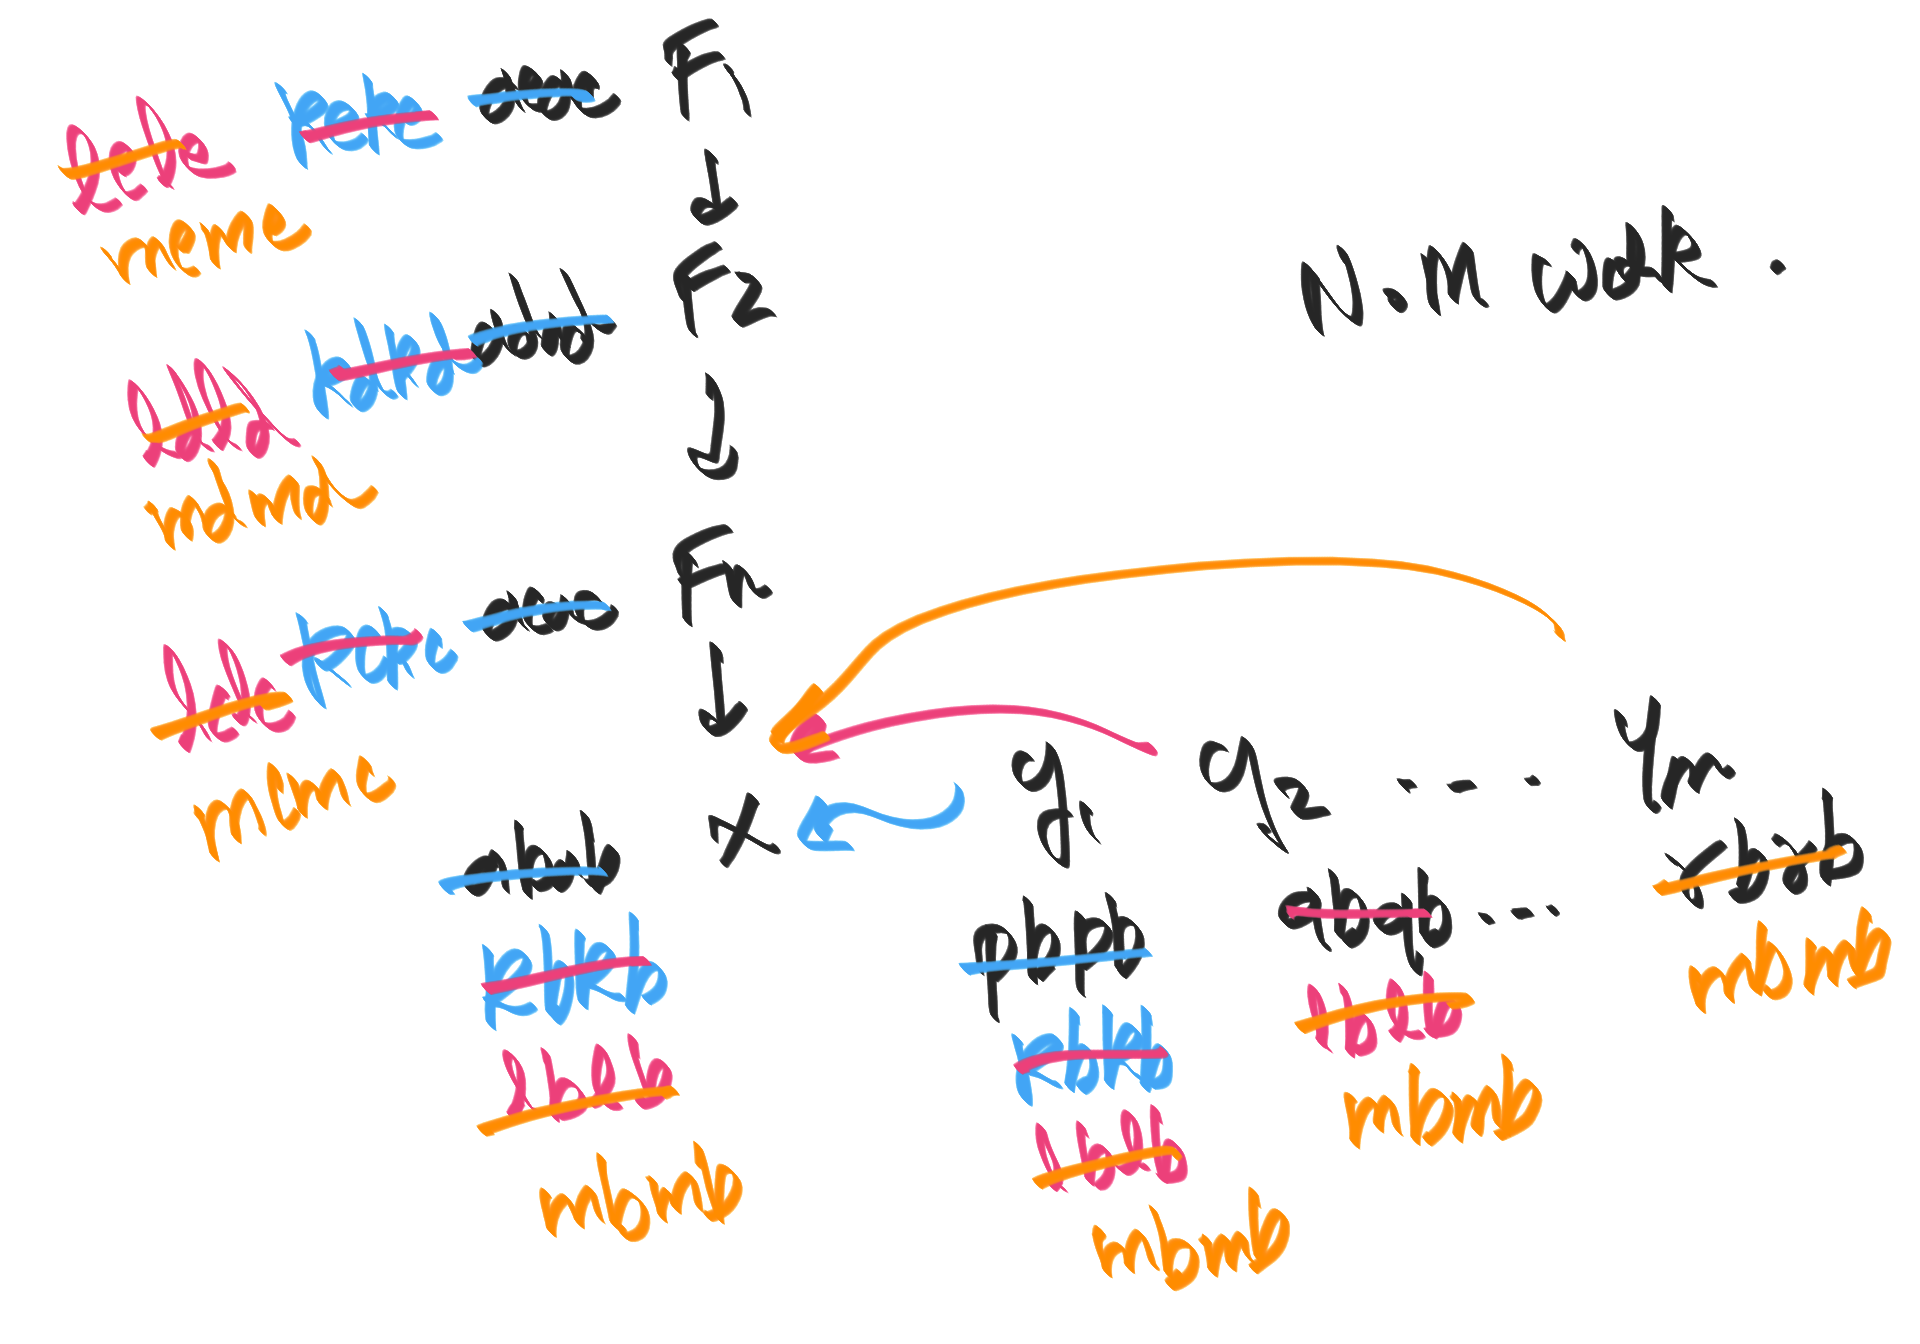
\includegraphics[width=\textwidth]{./eg-2-4.png}
\end{frame}


\begin{frame}[fragile]{Speedup over prior art: Merging}
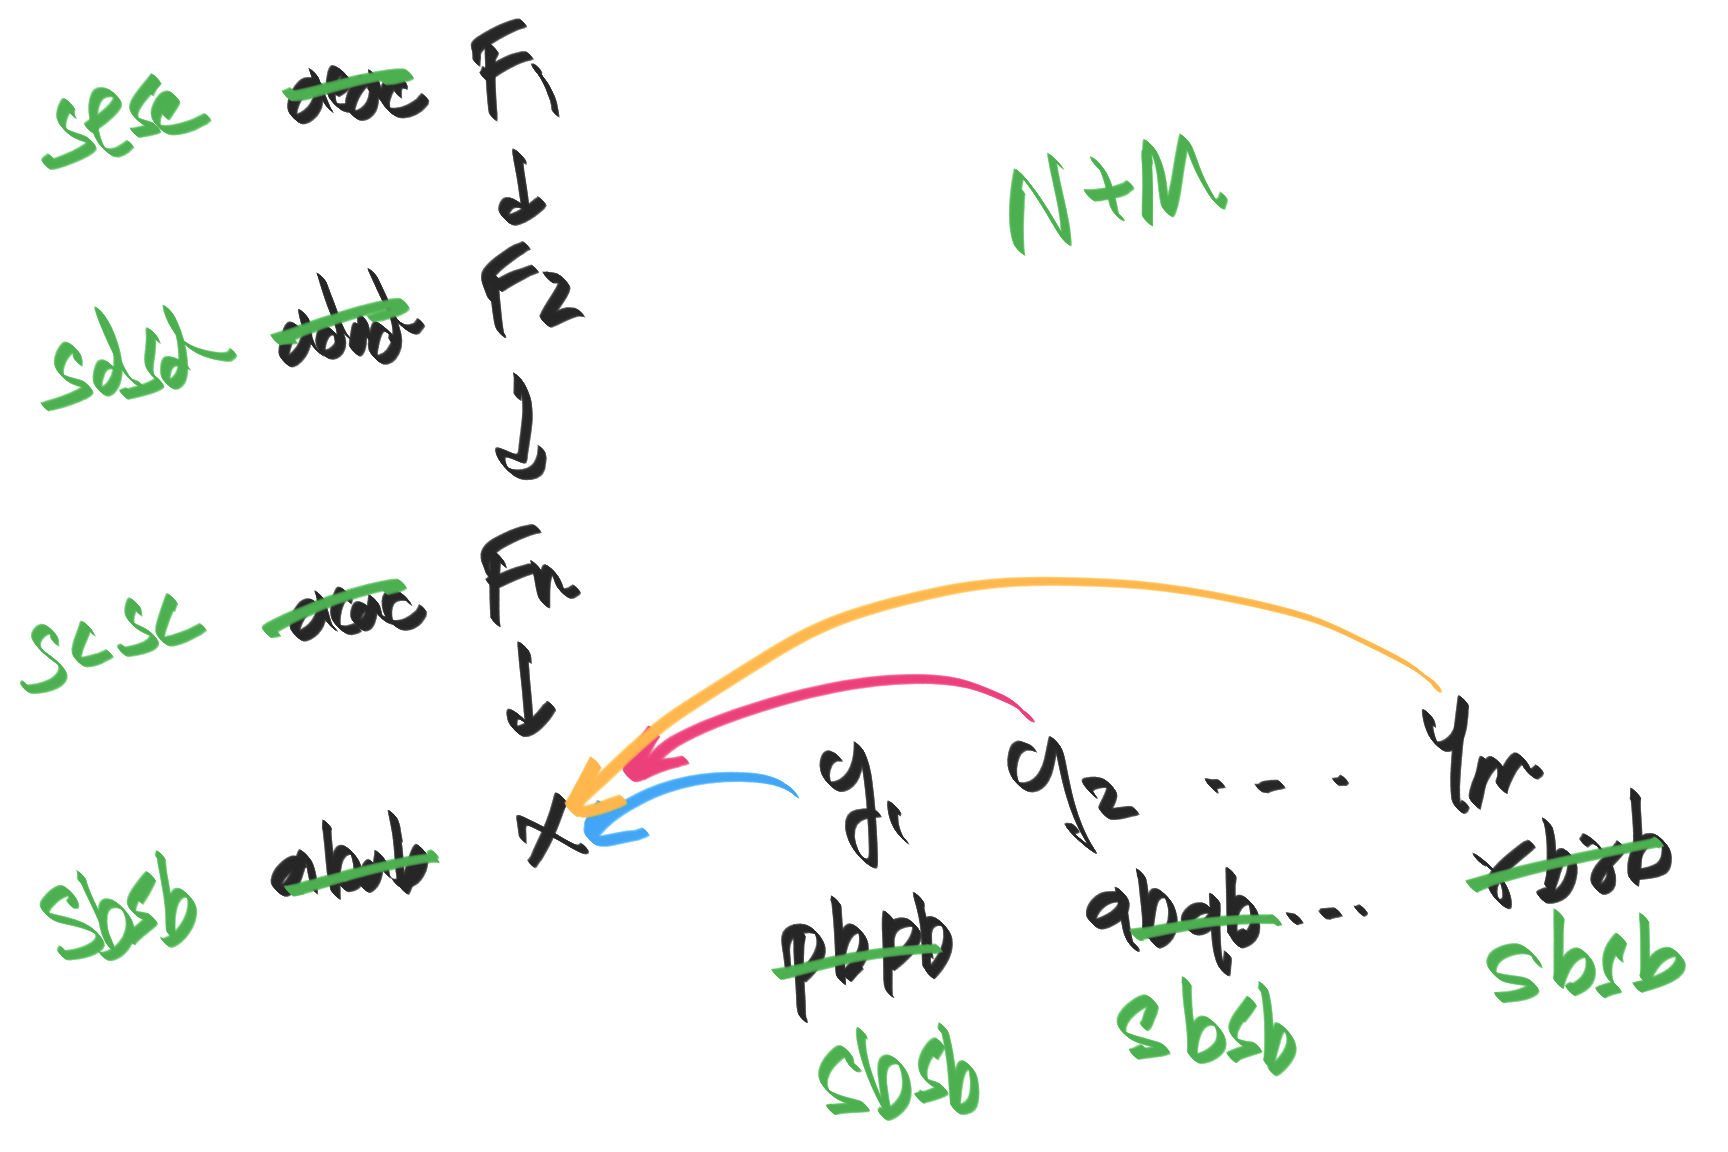
\includegraphics[width=\textwidth]{./eg-2-5.png}
\end{frame}


\begin{frame}[fragile]{Speedup over prior art: Merging}
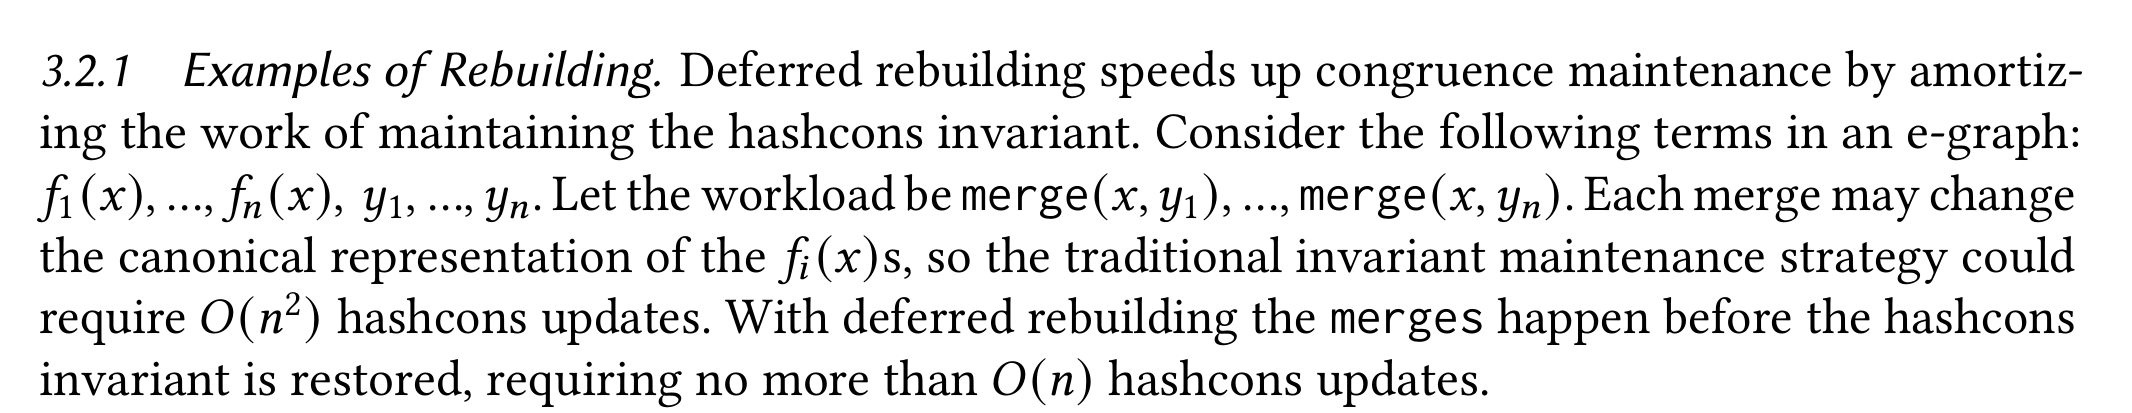
\includegraphics[width=\textwidth]{./eg-2-paper-snippet.png}
\end{frame}


\begin{frame}[fragile]{Takeaways}
\begin{itemize}
\item Don't stick to one order; try everything at once!
\item Solution to phase ordering!
\item Scales reasonably well if you engineer it well
\item Well-designed API that enables analysis and rewrites
\end{itemize}
\end{frame}

\begin{frame}[fragile]{Lambda calculus in \egg: Dynamic rewrites redux}
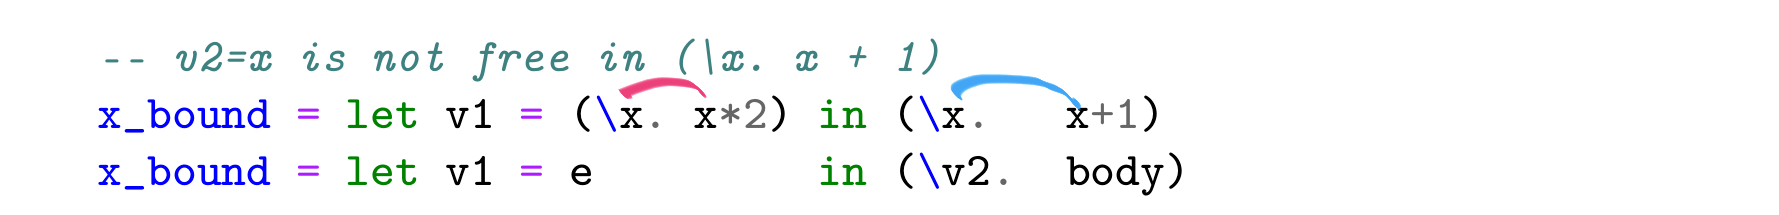
\includegraphics[width=\textwidth]{./lc-1.png}
\pause
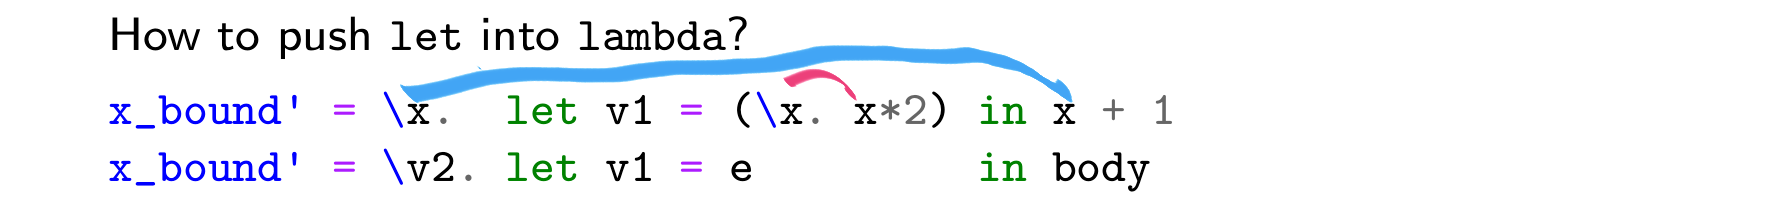
\includegraphics[width=\textwidth]{./lc-2.png}
\pause
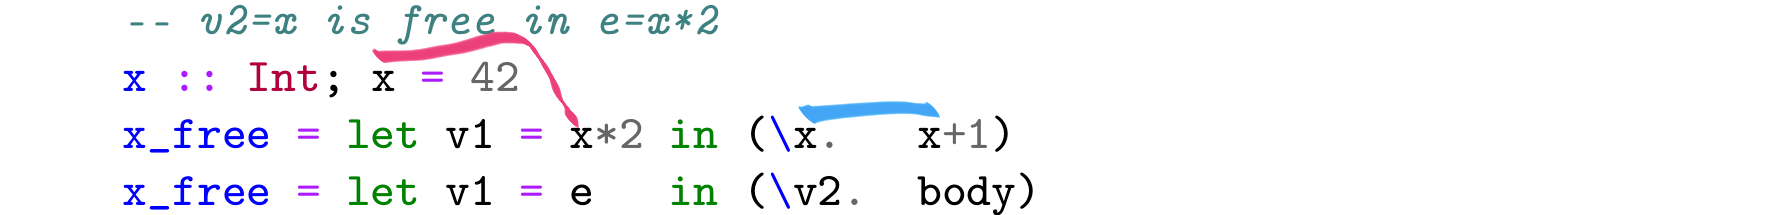
\includegraphics[width=\textwidth]{./lc-3.png}
\pause
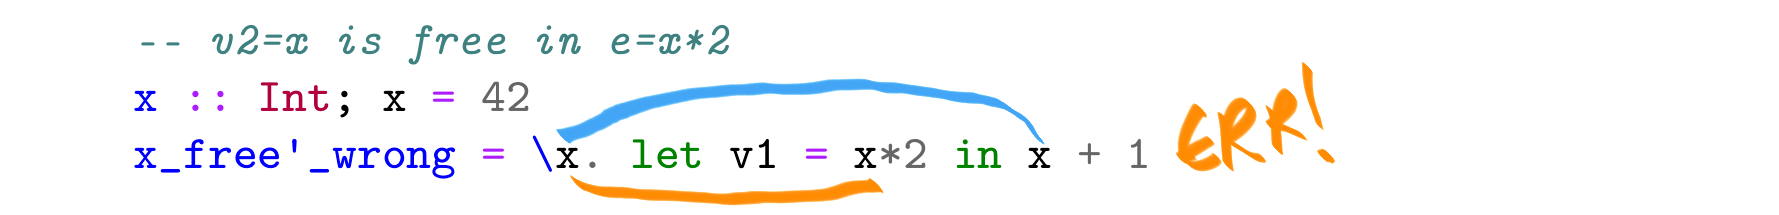
\includegraphics[width=\textwidth]{./lc-4.png}
\pause
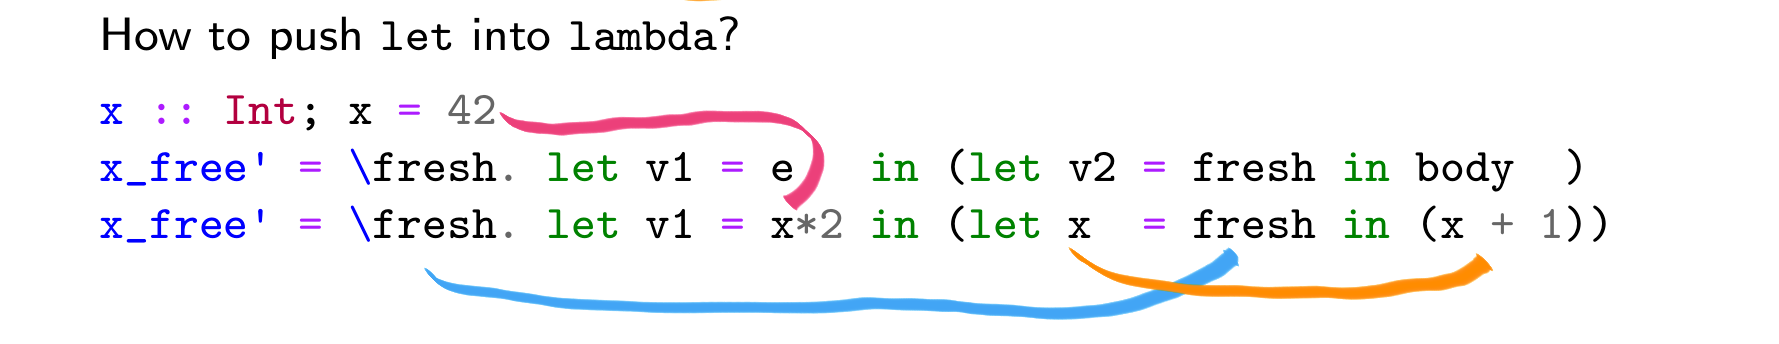
\includegraphics[width=\textwidth]{./lc-5.png}
\end{frame}

\begin{frame}[fragile]{Herbie: Using \egg --- Lattices}
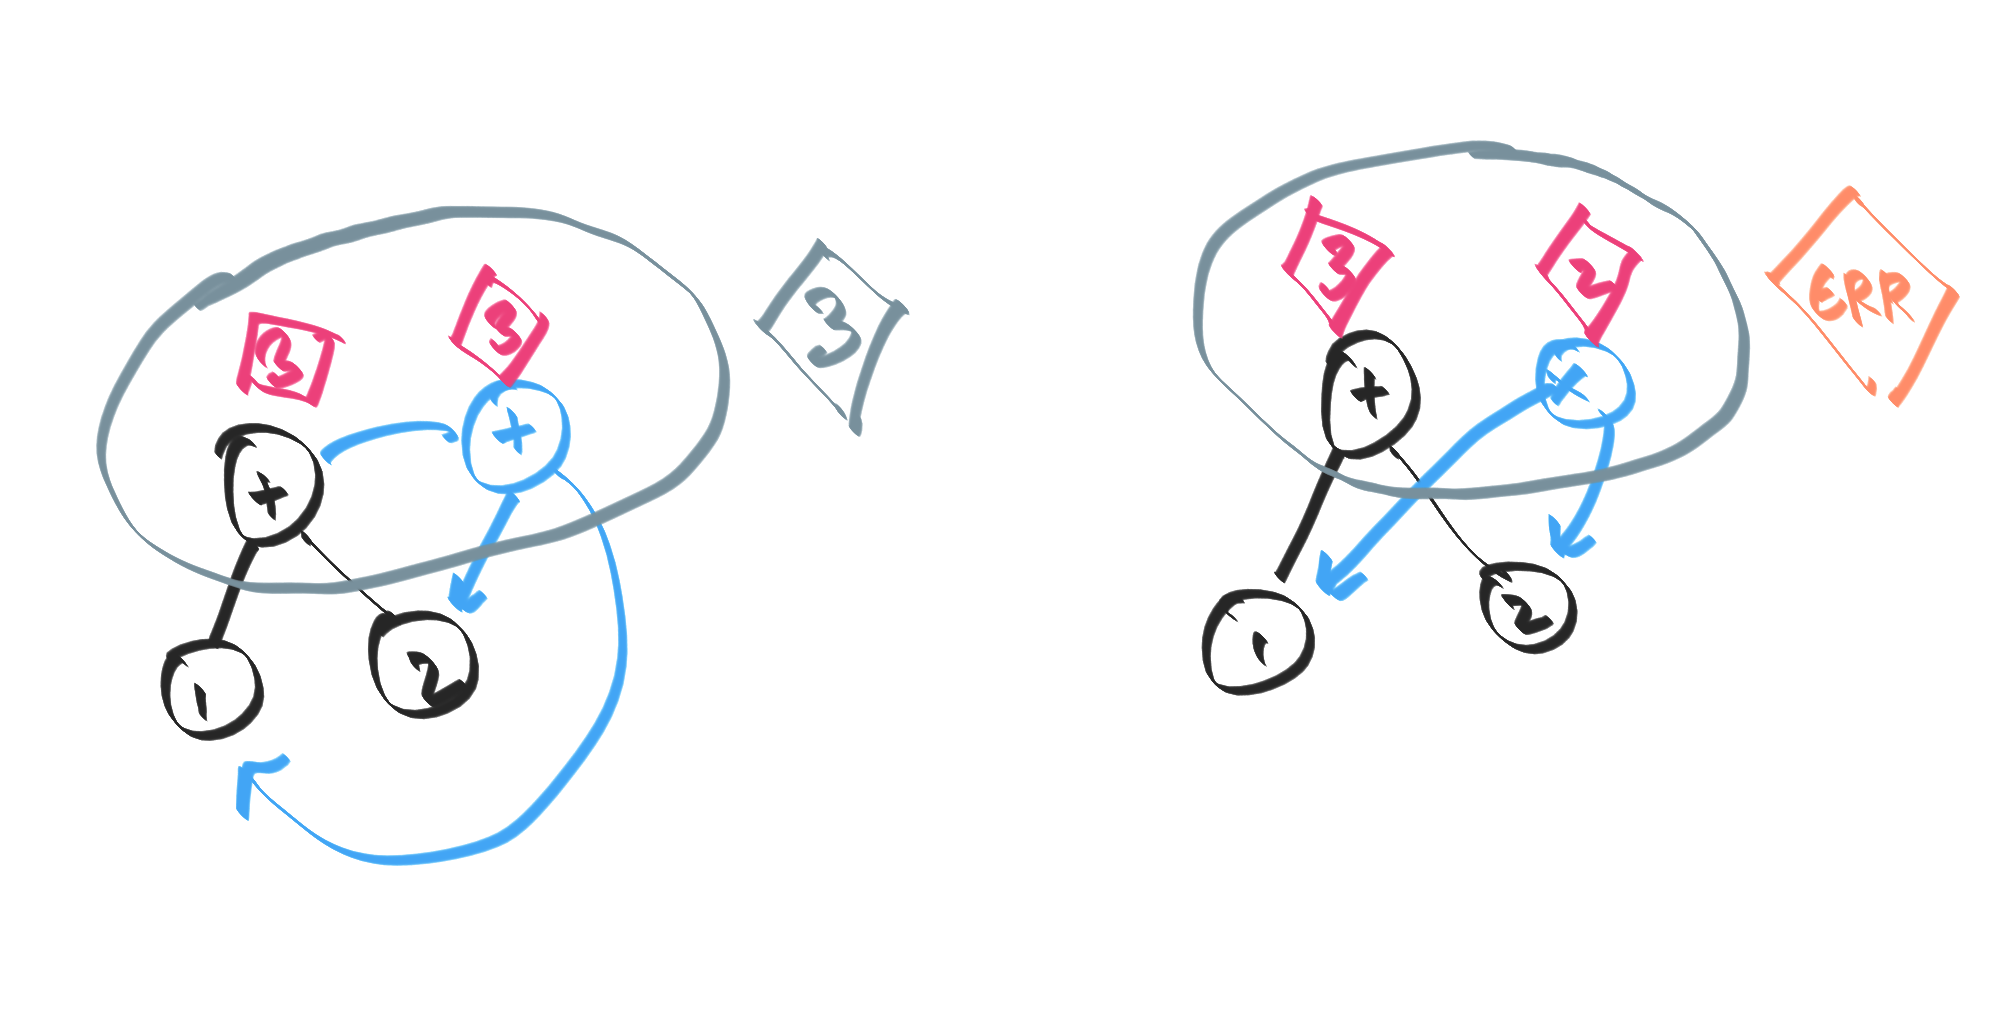
\includegraphics[width=\textwidth]{./analysis-equivalence-classes.png}
\pause
\begin{itemize}
\item Abstract interpretation of equivalence classes.
\item For each node, provide function $\alpha: \node \rightarrow L$ (Abstraction function)
\item $(L, \cap)$ is a join-semilattice.
\item \egg provides for each equivalence class $\class \mapsto \bigcap_{\node \in \class} \alpha(\node) \in L$
\end{itemize}
\end{frame}


\end{document}
